% Options for packages loaded elsewhere
% Options for packages loaded elsewhere
\PassOptionsToPackage{unicode}{hyperref}
\PassOptionsToPackage{hyphens}{url}
\PassOptionsToPackage{dvipsnames,svgnames,x11names}{xcolor}
%
\documentclass[
  polish,
  12pt,
  a4paper,
]{article}
\usepackage{xcolor}
\usepackage[margin=2.5cm]{geometry}
\usepackage{amsmath,amssymb}
\setcounter{secnumdepth}{5}
\usepackage{iftex}
\ifPDFTeX
  \usepackage[T1]{fontenc}
  \usepackage[utf8]{inputenc}
  \usepackage{textcomp} % provide euro and other symbols
\else % if luatex or xetex
  \usepackage{unicode-math} % this also loads fontspec
  \defaultfontfeatures{Scale=MatchLowercase}
  \defaultfontfeatures[\rmfamily]{Ligatures=TeX,Scale=1}
\fi
\usepackage{lmodern}
\ifPDFTeX\else
  % xetex/luatex font selection
\fi
% Use upquote if available, for straight quotes in verbatim environments
\IfFileExists{upquote.sty}{\usepackage{upquote}}{}
\IfFileExists{microtype.sty}{% use microtype if available
  \usepackage[]{microtype}
  \UseMicrotypeSet[protrusion]{basicmath} % disable protrusion for tt fonts
}{}
\makeatletter
\@ifundefined{KOMAClassName}{% if non-KOMA class
  \IfFileExists{parskip.sty}{%
    \usepackage{parskip}
  }{% else
    \setlength{\parindent}{0pt}
    \setlength{\parskip}{6pt plus 2pt minus 1pt}}
}{% if KOMA class
  \KOMAoptions{parskip=half}}
\makeatother
% Make \paragraph and \subparagraph free-standing
\makeatletter
\ifx\paragraph\undefined\else
  \let\oldparagraph\paragraph
  \renewcommand{\paragraph}{
    \@ifstar
      \xxxParagraphStar
      \xxxParagraphNoStar
  }
  \newcommand{\xxxParagraphStar}[1]{\oldparagraph*{#1}\mbox{}}
  \newcommand{\xxxParagraphNoStar}[1]{\oldparagraph{#1}\mbox{}}
\fi
\ifx\subparagraph\undefined\else
  \let\oldsubparagraph\subparagraph
  \renewcommand{\subparagraph}{
    \@ifstar
      \xxxSubParagraphStar
      \xxxSubParagraphNoStar
  }
  \newcommand{\xxxSubParagraphStar}[1]{\oldsubparagraph*{#1}\mbox{}}
  \newcommand{\xxxSubParagraphNoStar}[1]{\oldsubparagraph{#1}\mbox{}}
\fi
\makeatother


\usepackage{longtable,booktabs,array}
\usepackage{calc} % for calculating minipage widths
% Correct order of tables after \paragraph or \subparagraph
\usepackage{etoolbox}
\makeatletter
\patchcmd\longtable{\par}{\if@noskipsec\mbox{}\fi\par}{}{}
\makeatother
% Allow footnotes in longtable head/foot
\IfFileExists{footnotehyper.sty}{\usepackage{footnotehyper}}{\usepackage{footnote}}
\makesavenoteenv{longtable}
\usepackage{graphicx}
\makeatletter
\newsavebox\pandoc@box
\newcommand*\pandocbounded[1]{% scales image to fit in text height/width
  \sbox\pandoc@box{#1}%
  \Gscale@div\@tempa{\textheight}{\dimexpr\ht\pandoc@box+\dp\pandoc@box\relax}%
  \Gscale@div\@tempb{\linewidth}{\wd\pandoc@box}%
  \ifdim\@tempb\p@<\@tempa\p@\let\@tempa\@tempb\fi% select the smaller of both
  \ifdim\@tempa\p@<\p@\scalebox{\@tempa}{\usebox\pandoc@box}%
  \else\usebox{\pandoc@box}%
  \fi%
}
% Set default figure placement to htbp
\def\fps@figure{htbp}
\makeatother


% definitions for citeproc citations
\NewDocumentCommand\citeproctext{}{}
\NewDocumentCommand\citeproc{mm}{%
  \begingroup\def\citeproctext{#2}\cite{#1}\endgroup}
\makeatletter
 % allow citations to break across lines
 \let\@cite@ofmt\@firstofone
 % avoid brackets around text for \cite:
 \def\@biblabel#1{}
 \def\@cite#1#2{{#1\if@tempswa , #2\fi}}
\makeatother
\newlength{\cslhangindent}
\setlength{\cslhangindent}{1.5em}
\newlength{\csllabelwidth}
\setlength{\csllabelwidth}{3em}
\newenvironment{CSLReferences}[2] % #1 hanging-indent, #2 entry-spacing
 {\begin{list}{}{%
  \setlength{\itemindent}{0pt}
  \setlength{\leftmargin}{0pt}
  \setlength{\parsep}{0pt}
  % turn on hanging indent if param 1 is 1
  \ifodd #1
   \setlength{\leftmargin}{\cslhangindent}
   \setlength{\itemindent}{-1\cslhangindent}
  \fi
  % set entry spacing
  \setlength{\itemsep}{#2\baselineskip}}}
 {\end{list}}
\usepackage{calc}
\newcommand{\CSLBlock}[1]{\hfill\break\parbox[t]{\linewidth}{\strut\ignorespaces#1\strut}}
\newcommand{\CSLLeftMargin}[1]{\parbox[t]{\csllabelwidth}{\strut#1\strut}}
\newcommand{\CSLRightInline}[1]{\parbox[t]{\linewidth - \csllabelwidth}{\strut#1\strut}}
\newcommand{\CSLIndent}[1]{\hspace{\cslhangindent}#1}

\ifLuaTeX
\usepackage[bidi=basic]{babel}
\else
\usepackage[bidi=default]{babel}
\fi
% get rid of language-specific shorthands (see #6817):
\let\LanguageShortHands\languageshorthands
\def\languageshorthands#1{}


\setlength{\emergencystretch}{3em} % prevent overfull lines

\providecommand{\tightlist}{%
  \setlength{\itemsep}{0pt}\setlength{\parskip}{0pt}}



 


\usepackage{fontspec}
\usepackage{multirow}
\usepackage{multicol}
\usepackage{colortbl}
\usepackage{hhline}
\newlength\Oldarrayrulewidth
\newlength\Oldtabcolsep
\usepackage{longtable}
\usepackage{array}
\usepackage{hyperref}
\usepackage{float}
\usepackage{wrapfig}
\usepackage{booktabs}
\usepackage{float}
\usepackage{longtable}
\AtBeginDocument{\renewcommand{\emph}[1]{\textit{#1}}}
\makeatletter
\@ifpackageloaded{caption}{}{\usepackage{caption}}
\AtBeginDocument{%
\ifdefined\contentsname
  \renewcommand*\contentsname{Spis treści}
\else
  \newcommand\contentsname{Spis treści}
\fi
\ifdefined\listfigurename
  \renewcommand*\listfigurename{Spis rycin}
\else
  \newcommand\listfigurename{Spis rycin}
\fi
\ifdefined\listtablename
  \renewcommand*\listtablename{Spis tabel}
\else
  \newcommand\listtablename{Spis tabel}
\fi
\ifdefined\figurename
  \renewcommand*\figurename{Rysunek}
\else
  \newcommand\figurename{Rysunek}
\fi
\ifdefined\tablename
  \renewcommand*\tablename{Tabela}
\else
  \newcommand\tablename{Tabela}
\fi
}
\@ifpackageloaded{float}{}{\usepackage{float}}
\floatstyle{ruled}
\@ifundefined{c@chapter}{\newfloat{codelisting}{h}{lop}}{\newfloat{codelisting}{h}{lop}[chapter]}
\floatname{codelisting}{Wykaz}
\newcommand*\listoflistings{\listof{codelisting}{Spis wykazów}}
\makeatother
\makeatletter
\makeatother
\makeatletter
\@ifpackageloaded{caption}{}{\usepackage{caption}}
\@ifpackageloaded{subcaption}{}{\usepackage{subcaption}}
\makeatother
\usepackage{bookmark}
\IfFileExists{xurl.sty}{\usepackage{xurl}}{} % add URL line breaks if available
\urlstyle{same}
\hypersetup{
  pdftitle={Analiza bibliometryczna naukowców dyscypliny rolnictwo i ogrodnictwo w polskich uczelniach przyrodniczych z systemem Omega-PSIR},
  pdfauthor={Grzegorz Kulczycki},
  pdflang={pl},
  colorlinks=true,
  linkcolor={RoyalBlue},
  filecolor={Maroon},
  citecolor={RoyalBlue},
  urlcolor={RoyalBlue},
  pdfcreator={LaTeX via pandoc}}


\title{Analiza bibliometryczna naukowców dyscypliny rolnictwo i
ogrodnictwo w polskich uczelniach przyrodniczych z systemem Omega-PSIR}
\usepackage{etoolbox}
\makeatletter
\providecommand{\subtitle}[1]{% add subtitle to \maketitle
  \apptocmd{\@title}{\par {\large #1 \par}}{}{}
}
\makeatother
\subtitle{Praca dyplomowa: studia podyplomowe Data Science}
\author{Grzegorz Kulczycki}
\date{2026-06-20}
\begin{document}
% Partial Quarto: niestandardowa strona tytułowa (zastępuje domyślny \maketitle w PDF)
\begin{titlepage}
\thispagestyle{empty}
\centering

\vspace*{1cm}

\includegraphics[width=0.62\textwidth]{UEW_logo.png}

\vspace{2cm}
{\LARGE\bfseries Praca dyplomowa\par}

\vspace{0.4cm}
{\large Studia podyplomowe: Data Science\par}

\vspace{2.5cm}
{\Large\itshape Analiza bibliometryczna naukowców dyscypliny rolnictwo i
ogrodnictwo w polskich uczelniach przyrodniczych z systemem
Omega-PSIR\par}

\vfill

{\large Autor: Grzegorz Kulczycki\par}

\vspace{1.5cm}
{\normalsize Wrocław, 2026\par}

\vspace{1cm}
\end{titlepage}
\renewcommand*\contentsname{Spis treści}
{
\hypersetup{linkcolor=RoyalBlue}
\setcounter{tocdepth}{3}
\tableofcontents
}

\newpage{}

\section*{Streszczenie}\label{streszczenie}
\addcontentsline{toc}{section}{Streszczenie}

Praca analizuje dorobek publikacyjny 462 pracowników z dyscypliny
rolnictwo i ogrodnictwo z czterech polskich uczelni przyrodniczych:
UPWr, SGGW, URK i UWM. Wykorzystano dane z systemu Omega-PSIR, a
następnie uzupełniono je informacjami z bazy OpenAlex, między innymi o
wskaźnik wpływu publikacji i dane o współautorstwie.

Analiza obejmowała cztery części: porównanie wyników między uczelniami i
stanowiskami, podział pracowników na podobne profile publikacyjne,
przewidywanie wysokiego wpływu naukowego oraz badanie sieci współpracy
między autorami.

Badania wykazały, że dorobek indywidualny i współpraca naukowa zależą od
różnych czynników. \textbf{Indywidualne osiągnięcia publikacyjne zależą
głównie od etapu kariery}: im wyższe stanowisko, tym większy dorobek, i
widać to podobnie na wszystkich uczelniach. Natomiast \textbf{współpraca
między autorami zależy głównie od uczelni}: badacze najczęściej
współpracują w ramach swojej afiliacji, a nie według stanowiska. Wysoki
wpływ można dość dobrze przewidzieć na podstawie cech badacza.
Najważniejsze są produktywność i pozycja w sieci współpracy, a nie samo
stanowisko formalne. Model rozróżnia osoby o wysokim i niższym wpływie
skumulowanym bardzo skutecznie, osiągając AUC około 0,97, przy czym ten
cel jest po części pochodną liczby publikacji. Gdy celem jest jakość
niekumulatywna (intensywność cytowań niezależna od dorobku), predykcja
jest wyraźnie trudniejsza (AUC około 0,81) i zależy nie od stażu, lecz
od struktury współpracy. Wyniki potwierdzają także, że jednorodność i
kompletność danych są warunkiem wiarygodnego wnioskowania, ważniejszym
niż wygoda gotowych indeksów globalnych: ten sam wskaźnik tempa rozwoju
prowadzi do przeciwnych wniosków, gdy dane są niepełne. W polskim
szkolnictwie wyższym systemy klasy CRIS, takie jak Omega-PSIR, są więc
bezpieczniejszą podstawą porównań międzyuczelnianych niż bazy globalne.

\textbf{Słowa kluczowe:} bibliometria, naukometria, Omega-PSIR,
OpenAlex, rolnictwo i ogrodnictwo, ewaluacja nauki, klastrowanie, sieci
współautorstwa, uczenie maszynowe.

\newpage{}

\section{Wprowadzenie}\label{wprowadzenie}

\subsection{Kontekst: ewaluacja jakości działalności naukowej w
Polsce}\label{kontekst-ewaluacja-jakoux15bci-dziaux142alnoux15bci-naukowej-w-polsce}

Polski system oceny nauki opiera się na okresowej \textbf{ewaluacji
jakości działalności naukowej}, przeprowadzanej co cztery lata przez
Komisję Ewaluacji Nauki na podstawie danych zgromadzonych w systemie
POL-on (\citeproc{ref-rozp_ewaluacja2022}{Minister Edukacji i Nauki
2022}). Ewaluacja nie ocenia pojedynczych naukowców, lecz
\textbf{podmioty (uczelnie, instytuty) w obrębie poszczególnych
dyscyplin naukowych}, nadając każdej parze podmiot--dyscyplina kategorię
naukową (A+, A, B+, B lub C). Kategoria przekłada się bezpośrednio na
uprawnienia jednostki, m.in. prawo do nadawania stopni naukowych oraz
wysokość finansowania.

Punktem odniesienia dla całego systemu jest urzędowa
\textbf{klasyfikacja dziedzin i dyscyplin naukowych}; analizowana w
niniejszej pracy dyscyplina rolnictwo i ogrodnictwo należy do dziedziny
nauk rolniczych (\citeproc{ref-rozp_dyscypliny2025}{Minister Nauki i
Szkolnictwa Wyższego 2025a}). Ocena w ewaluacji opiera się na trzech
kryteriach: (I) poziomie naukowym prowadzonej działalności, mierzonym
punktacją ministerialną publikacji i patentów, (II) efektach finansowych
badań naukowych oraz (III) wpływie działalności naukowej na
funkcjonowanie społeczeństwa i gospodarki. Wagi kryteriów różnią się
między dziedzinami; dla nauk rolniczych Kryterium I waży 50 \%,
Kryterium II 35 \%, a Kryterium III 15 \% oceny
(\citeproc{ref-rozp_ewaluacja2022}{Minister Edukacji i Nauki 2022};
\citeproc{ref-rozp_ewaluacja_nowela2025}{Minister Nauki i Szkolnictwa
Wyższego 2025b}). Kryterium I, dominujące w naukach rolniczych, ma
charakter bibliometryczny: liczbę punktów wyznacza się z udziałów
jednostkowych autorów w publikacjach, w ramach limitu slotów
publikacyjnych proporcjonalnego do liczby pracowników danej dyscypliny
(liczby N).

Rozporządzenie klasyfikacyjne wymienia dyscypliny wyłącznie z nazwy, nie
wyznaczając formalnie ich zakresu przedmiotowego
(\citeproc{ref-rozp_dyscypliny2025}{Minister Nauki i Szkolnictwa
Wyższego 2025a}). Rolnictwo i ogrodnictwo jest jedną z czterech
dyscyplin dziedziny nauk rolniczych (obok nauk leśnych, technologii
żywności i żywienia oraz zootechniki i rybactwa) i powstało przy
reformie klasyfikacji z 2018 r. ze scalenia węższych, wcześniej
odrębnych dyscyplin, przede wszystkim agronomii i ogrodnictwa. Jej
merytoryczny trzon stanowią nauki o roślinie uprawnej i o środowisku jej
wzrostu: produkcja roślinna i agrotechnika, ogrodnictwo (warzywnictwo,
sadownictwo, rośliny ozdobne), gleboznawstwo i żywienie roślin, ochrona
roślin, hodowla i genetyka roślin, łąkarstwo oraz kształtowanie i
ochrona agrocenoz. Poza zakresem dyscypliny pozostają produkcja
zwierzęca (przypisana do zootechniki i rybactwa) oraz przetwórstwo
płodów rolnych (technologia żywności i żywienia), co czyni rolnictwo i
ogrodnictwo przede wszystkim roślinno-środowiskowym segmentem nauk
rolniczych.

Ponieważ ewaluacja nauki w dużej mierze opiera się na wskaźnikach
bibliometrycznych, takich jak punktacja ministerialna, cytowania i
liczba publikacji, indywidualne profile dorobku naukowców są ważnym
przedmiotem analizy. Analiza bibliometryczna jest w Polsce
wykorzystywana zarówno w polityce naukowej i ewaluacji
(\citeproc{ref-Drabek2012}{Drabek 2012};
\citeproc{ref-Kulczycki2019}{Kulczycki 2019}), jak i do oceny dorobku
pracowników poszczególnych uczelni (\citeproc{ref-Grygiel2009}{Grygiel,
Rębisz, i Humenny 2009}); polskie piśmiennictwo dysponuje też
przeglądami metod bibliometrycznych stosowanych do oceny i prognozowania
rozwoju dyscyplin naukowych (\citeproc{ref-Opalinski2017}{Opaliński
2017}). Niniejsza praca nie odtwarza oficjalnego algorytmu ewaluacji,
który działa na poziomie uczelni i dyscypliny. Analizuje natomiast
zróżnicowanie indywidualnych profili bibliometrycznych pracowników
prowadzących działalność naukową w tej samej dyscyplinie, a kategorię
naukową uczelni traktuje jako zmienną opisową.

\newpage{}

\subsection{Cel pracy}\label{cel-pracy}

Niniejsza praca analizuje dorobek bibliometryczny pracowników naukowych
dyscypliny rolnictwo i ogrodnictwo w czterech polskich uczelniach
przyrodniczych: Uniwersytecie Przyrodniczym we Wrocławiu (UPWr,
kategoria A), Szkole Głównej Gospodarstwa Wiejskiego w Warszawie (SGGW,
A), Uniwersytecie Rolniczym im. Hugona Kołłątaja w Krakowie (URK, A)
oraz Uniwersytecie Warmińsko-Mazurskim w Olsztynie (UWM, B+). Wszystkie
te uczelnie korzystają z systemu Omega-PSIR jako Bazy Wiedzy. Nazwa
Omega-PSIR określa przy tym sam system informatyczny (CRIS), natomiast
jego wdrożenie i publiczny portal na poszczególnych uczelniach
funkcjonują pod nazwą Baza Wiedzy.

Omega-PSIR jest systemem klasy CRIS (\emph{Current Research Information
System}), opracowanym na Politechnice Warszawskiej w ramach prac nad
Bazą Wiedzy PW. System powstał w zespole Politechniki Warszawskiej w
ramach projektu SYNAT (finansowanego przez NCBiR), którego celem było
zbudowanie otwartej infrastruktury repozytoryjno-informacyjnej dla
polskiej nauki; pierwsze wdrożenia produkcyjne na Politechnice
Warszawskiej uruchomiono w latach 2011--2013 (od 2013 r. system objął
całą uczelnię) (\citeproc{ref-koperwas2015omega}{Koperwas i in. 2015}).
Pełni funkcję repozytorium instytucjonalnego oraz narzędzia
wspierającego zarządzanie informacją o działalności naukowej uczelni:
gromadzi dane o publikacjach, projektach, patentach, raportach,
rozprawach doktorskich, metrykach bibliometrycznych i afiliacjach
pracowników. Według stanu na 2018 r. system był wdrożony w kilkunastu
polskich instytucjach naukowych (Politechnika Warszawska i jedenaście
innych uczelni)
(\citeproc{ref-rybinskiOmegaPSIRInstitutionalCRIS2018}{Rybiński i in.
2018}) i jest dostosowany do krajowego systemu ewaluacji nauki. Jego
znaczenie dla niniejszej pracy polega na tym, że udostępnia
porównywalne, uczelniane agregaty dorobku naukowego w jednolitej
strukturze danych (\citeproc{ref-omegapsir2024}{Warsaw University of
Technology 2024}).

Kryterium doboru próby jest \textbf{jednolitość systemu informacji o
nauce}: wszystkie cztery uczelnie korzystają z polskiego CRIS-u
Omega-PSIR, co zapewnia identyczną procedurę pozyskania danych, te same
kategorie pól bibliometrycznych i porównywalność wskaźników. W doborze
próby ważniejsza od jednorodności kategorii ewaluacyjnej była
porównywalność samego źródła danych. Różne systemy CRIS mogą mieć
odmienne zasady gromadzenia publikacji, co może prowadzić do
nieporównywalnych metryk. Pokazał to test kompletności wykonany na
etapie projektowania badania: DSpace-CRIS Uniwersytetu Przyrodniczego w
Poznaniu obejmował tylko około 10--15 \% dorobku widocznego w systemach
Omega-PSIR. Kategorii ewaluacyjnej MEiN nie analizowano jako osobnej
zmiennej, ponieważ w tej próbie jest ona \textbf{idealnie współliniowa z
uczelnią}: tylko UWM ma kategorię B+, a pozostałe trzy uczelnie mają
kategorię A. Nie można więc rozstrzygnąć, czy ewentualne różnice
wynikają z kategorii, czy ze specyfiki danej uczelni. Z tego powodu
kategorię MEiN potraktowano \textbf{wyłącznie opisowo}, a wynikające z
tego ograniczenie omówiono w rozdziale Dyskusja.

Pominięto Uniwersytet Przyrodniczy w Poznaniu (kategoria A, DSpace) z
powodu niekompletności jego CRIS-u oraz Zachodniopomorski Uniwersytet
Technologiczny w Szczecinie (kategoria A) ze względu na brak publicznie
dostępnego CRIS-u. Uniwersytet Przyrodniczy w Lublinie (B+) został
pominięty ze względu na własny system OpenUP o asymetrycznej metodyce
ekstrakcji.

\newpage{}

\subsection{Pytania badawcze}\label{pytania-badawcze}

\textbf{1.} Czy badani naukowcy tworzą odrębne typy profili
bibliometrycznych?

\textbf{2.} W jakim stopniu stanowisko naukowe i uczelnia różnicują ich
wskaźniki bibliometryczne?

\textbf{3.} Czy da się przewidzieć wysoki wpływ dorobku naukowca na
podstawie jego stanowiska, uczelni, liczby publikacji i współpracy z
innymi autorami?

\textbf{4.} Czy sieć współautorstwa ma charakter głównie
wewnątrzuczelniany, czy widoczne są także wspólnoty międzyuczelniane?

\section{Materiał i metodyka}\label{materiaux142-i-metodyka}

\subsection{Źródła danych}\label{ux17aruxf3dux142a-danych}

\begin{itemize}
\item
  \textbf{Omega-PSIR (4 instancje uczelniane)}
  (\citeproc{ref-omegapsir2024}{Warsaw University of Technology 2024}),
  źródło podstawowe: agregaty bibliometryczne per autor (h-index
  WoS/Scopus (\citeproc{ref-hirsch2005}{Hirsch 2005}), sumaryczny IF
  (\citeproc{ref-garfield2006}{Garfield 2006}), SNIP
  (\citeproc{ref-moed2010snip}{Moed 2010}), punktacja
  MEiN/ministerialna, liczba publikacji), dane afiliacyjne (jednostka,
  wydział, stanowisko), identyfikatory ORCID.
\item
  \textbf{OpenAlex API} (\citeproc{ref-openalex2022}{Priem, Piwowar, i
  Orr 2022}), źródło uzupełniające, dostarcza danych, których nie ma w
  Omega-PSIR: FWCI (Field-Weighted Citation Impact), czyli
  znormalizowany dziedzinowo wskaźnik cytowań odnoszący liczbę cytowań
  pracy do światowej średniej w jej dziedzinie (wartość 1,0 oznacza
  poziom średniej światowej, a wartości powyżej 1,0 wynik ją
  przewyższający), którego nie da się policzyć z danych jednej uczelni
  (\citeproc{ref-waltman2016review}{Waltman 2016}); liczbę cytowań
  publikacji; listę współautorów potrzebną do analizy sieci współpracy;
  oraz niezależne porównanie (kontrolę jakości) metryk pobranych z
  Omega-PSIR.
\end{itemize}

Dla każdego autora analizowano podstawowe wskaźniki bibliometryczne,
takie jak sumaryczny IF, punktacja MEiN, h-index i liczba publikacji.

Należy zaznaczyć, że wskaźniki te służą jako przybliżenie indywidualnego
dorobku naukowego, a nie jako odtworzenie oficjalnej ewaluacji jakości
działalności naukowej; ostrożność w traktowaniu pojedynczych wskaźników
jako miar jakości naukowej jest zgodna z zasadami odpowiedzialnej
naukometrii (\citeproc{ref-hicksBibliometricsLeidenManifesto2015}{Hicks
i in. 2015}). Oficjalna ewaluacja prowadzona jest na poziomie uczelni i
dyscypliny, uwzględnia udziały jednostkowe autorów oraz limity slotów
publikacyjnych (3-krotność liczby N), a jej podstawą nie jest Impact
Factor, lecz punktacja ministerialna czasopism
(\citeproc{ref-rozp_ewaluacja2022}{Minister Edukacji i Nauki 2022}).

Wskaźniki wykorzystane w tej pracy wybrano dlatego, że są dostępne w
porównywalnej formie dla badanych uczelni i pozwalają opisać profil
bibliometryczny naukowca.

\subsection{Procedura pozyskania
danych}\label{procedura-pozyskania-danych}

Pozyskanie i przygotowanie danych przeprowadzono według jednolitej
procedury (Rysunek~\ref{fig-pipeline}). Dane bibliometryczne pobrano z
czterech uczelnianych instancji systemu Omega-PSIR za pomocą autorskiego
scrapera napisanego w Pythonie, wykorzystującego bibliotekę Playwright i
przeglądarkę Chromium.

Wyboru tego narzędzia wymagała architektura portali: strony Omega-PSIR
(oparte na frameworku PrimeFaces) ładują część treści dynamicznie, więc
zwykłe pobranie kodu HTML nie wystarczało do poprawnej ekstrakcji
danych. Sterowanie pełną przeglądarką pozwala poczekać, aż profil autora
oraz lista wyników w pełni się załadują, i dopiero wtedy odczytać dane.

Scraper działał w dwóch etapach. W pierwszym etapie przechodził przez
listę pracowników odfiltrowaną do dyscypliny rolnictwo i ogrodnictwo i
zbierał identyfikatory autorów. W drugim etapie otwierał profil każdego
autora i pobierał dane bibliometryczne, afiliacyjne oraz identyfikator
ORCID.

Szczególnym problemem była paginacja listy autorów. Kolejne strony
wyników nie miały stabilnych adresów URL, dlatego scraper przechodził
przez nie tak, jak użytkownik: programowo klikając przycisk „następna
strona''. Dzięki temu możliwe było zebranie identyfikatorów wszystkich
autorów z wybranej dyscypliny.

Kod scrapera podzielono na część wspólną i konfiguracje dla
poszczególnych uczelni. Część wspólna odpowiadała za nawigację,
oczekiwanie na załadowanie strony i ekstrakcję danych, natomiast
konfiguracje uczelniane uwzględniały drobne różnice między instancjami
Omega-PSIR, takie jak nazwy pól czy czas ładowania profilu. Proces
zabezpieczono autozapisem postępu, możliwością wznowienia pracy po
przerwaniu oraz ponawianiem nieudanych prób pobrania danych.

Dla każdej uczelni zapisano osobny plik CSV. Następnie dane zostały
ujednolicone, oczyszczone z duplikatów oraz pozbawione rekordów osób,
które nie były pracownikami naukowymi. Po tym etapie końcowa próba
analityczna liczyła 462 osoby.

Po oczyszczeniu danych z Omega-PSIR uzupełniono je informacjami z
OpenAlex. Najpierw dopasowano autorów z badanej próby do rekordów w
OpenAlex, wykorzystując identyfikator instytucji ROR oraz podobieństwo
imienia i nazwiska. Oparcie powiązania na kanonicznych identyfikatorach
(ROR dla instytucji, ORCID dla autorów) jest zgodne z podejściem
stosowanym w dedykowanych narzędziach integracji danych OpenAlex w
środowisku R (\citeproc{ref-ariaOpenalexR2024}{Aria i in. 2024}).
Następnie dla dopasowanych autorów pobrano informacje o publikacjach,
cytowaniach, wskaźniku FWCI oraz współautorach. Zapytania do OpenAlex
wykonywano z ograniczeniem tempa i identyfikacją użytkownika, zgodnie z
zasadami korzystania z API.

Dane z Omega-PSIR i OpenAlex połączono w jeden zbiór analityczny
(\texttt{profiles\_features.csv}). Osobno, na potrzeby analizy dynamiki
publikacyjnej, pobrano pełne listy publikacji z systemu Omega-PSIR dla
wszystkich zeskrapowanych osób (491, przed odsianiem), wraz z rokiem
publikacji i punktacją. Dane między skryptami Python i R przekazywano w
formacie CSV.

\begin{figure}[H]

\centering{

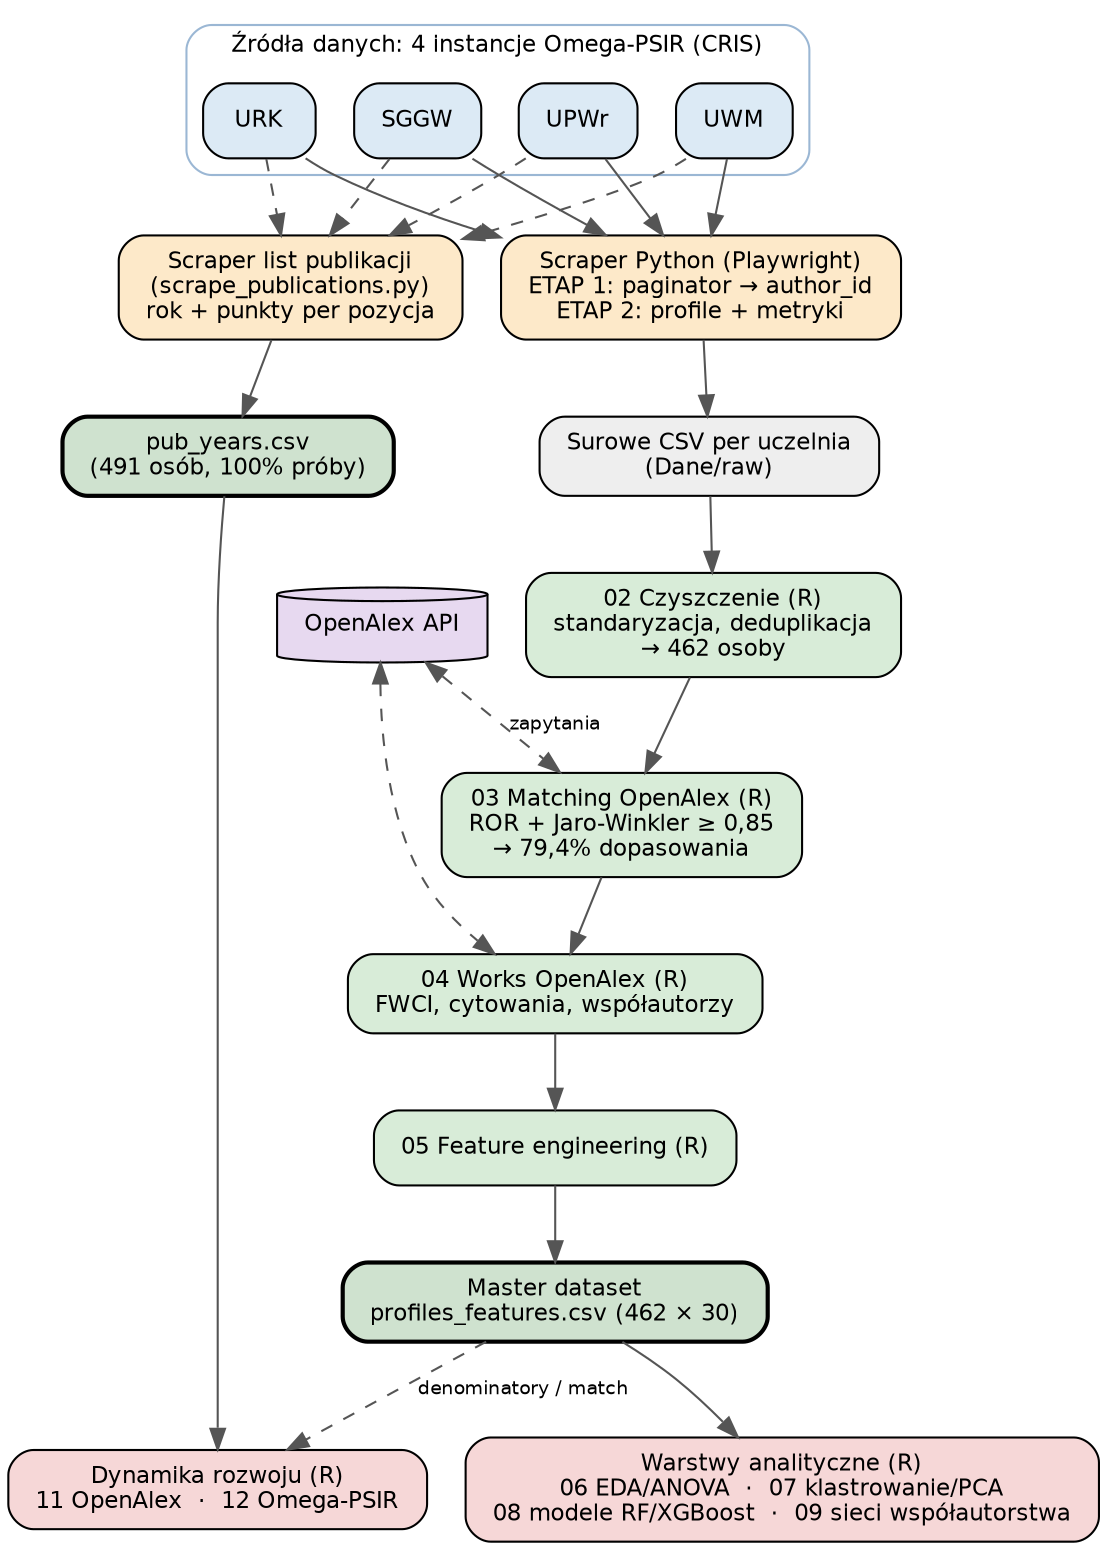
\includegraphics[width=0.84\linewidth,height=\textheight,keepaspectratio]{../Wykresy/praca/fig_00_pipeline.png}

}

\caption{\label{fig-pipeline}Schemat przepływu danych: od czterech
instancji Omega-PSIR przez scraping (Python) i przetwarzanie (R) z
uzupełnieniem OpenAlex do zbioru analitycznego i warstw modelowania.}

\end{figure}%

\subsection{Metody analityczne}\label{metody-analityczne}

Całość analizy zorganizowano zgodnie z typowym dla badań
bibliometrycznych przepływem pracy: projektowanie badania, gromadzenie i
łączenie danych, analiza, wizualizacja oraz interpretacja
(\citeproc{ref-ariaBibliometrix2017}{Aria i Cuccurullo 2017}).
Obliczenia zaimplementowano samodzielnie w językach Python i R (bez
gotowych pakietów do mapowania nauki), korzystając z bibliotek ogólnego
przeznaczenia opisanych niżej.

\begin{itemize}
\tightlist
\item
  \emph{Analiza opisowa i statystyczna:} obejmowała porównanie
  wskaźników między uczelniami i stanowiskami. Założenia parametryczne
  sprawdzono testami Shapiro-Wilka (normalność reszt modelu w układzie
  dwuczynnikowym) i Levene'a (jednorodność wariancji); ponieważ dla
  wszystkich sześciu metryk zostały one naruszone, zastosowano
  \textbf{ścieżkę nieparametryczną}: ogólny test Kruskala-Wallisa dla 12
  grup utworzonych przez połączenie uczelni i stanowisk, a następnie,
  dla metryk z istotnym wynikiem tego testu, post-hoc Dunna z korektą
  Bonferroniego. Należy zaznaczyć, że Kruskal-Wallis na komórkach
  porównuje 12 grup łącznie i nie rozdziela formalnie efektów głównych
  od interakcji. Grupy jednorodne (compact letter display) wyznaczano
  metodą \texttt{multcompLetters} na macierzy istotności porównań
  parami. Pomocniczo, na potrzeby ryciny rozkładów, ten sam test Dunna z
  korektą Bonferroniego przeprowadzono w dwóch symetrycznych wariantach
  jednoczynnikowych: w obrębie każdej uczelni osobno (porównanie
  stanowisk, małe litery CLD) oraz w obrębie każdego stanowiska osobno
  (porównanie uczelni, duże litery CLD); każdy wariant kontroluje drugi
  czynnik, ilustrując różnice między stanowiskami i między uczelniami
  niezależnie od siebie. Poziom \emph{asystent} (n = 26, nieobecny w UWM
  i UPWr) wykluczono z analizy interakcji. Metryki oparte na punktacji
  MEiN analizowano na trzech uczelniach (SGGW nie eksponuje sum\_MEiN w
  API, 100 \% braków danych).
\item
  \emph{Analiza PCA i klastrowanie k-means:} podział naukowców na grupy
  o podobnych profilach bibliometrycznych. Cechy o pełnym pokryciu
  czterech uczelni (h-index WoS, sumaryczny IF, IF na publikację, liczba
  publikacji), z pominięciem metryk MEiN, które wykluczyłyby całą próbę
  SGGW. Obok rozwiązania głównego (k z sylwetki) zbadano wariant
  eksploracyjny k = 3.
\item
  \emph{Modelowanie predykcyjne:} do przewidywania wysokiego wpływu
  zastosowano modele Random Forest (\citeproc{ref-breiman2001}{Breiman
  2001}) i XGBoost (\citeproc{ref-chen2016}{Chen i Guestrin 2016}). Ich
  jakość oceniono w 5-krotnej walidacji krzyżowej (dane uczące dzielono
  na pięć części i każdą wykorzystano raz jako zbiór sprawdzający,
  uśredniając wyniki), co pozwoliło dobrać hiperparametry modeli bez
  dopasowywania ich do pojedynczego podziału danych. Znaczenie cech
  opisano za pomocą wartości SHAP (\citeproc{ref-lundberg2017}{Lundberg
  i Lee 2017}). Zbudowano dwa modele o rozłącznych celach:
  \textbf{ilościowy} (wysoki sumaryczny wpływ, kumulatywny) oraz
  \textbf{jakościowy} (wysoka intensywność cytowań niezależna od
  dorobku: FWCI \textgreater{} 1, czyli powyżej światowej średniej w
  dziedzinie). W modelu jakościowym dołączono jawnie cechę \textbf{wieku
  akademickiego} (lata od pierwszej publikacji wg OpenAlex), by
  sprawdzić, czy jakość daje się sprowadzić do stażu.
\item
  \emph{Analiza sieci współautorstwa:} sprawdzono, którzy badacze
  publikują razem i czy tworzą większe grupy współpracy
  (\citeproc{ref-newmanCoauthorshipNetworksPatterns2004}{Newman 2004}).
  Do wykrycia takich grup zastosowano algorytm Louvain
  (\citeproc{ref-blondel2008}{Blondel i in. 2008}), a modularność
  (\citeproc{ref-newman2006}{Newman 2006}) wykorzystano do oceny, jak
  wyraźnie sieć dzieli się na wspólnoty. Dzięki temu można było
  sprawdzić, czy współpraca przebiega głównie w obrębie jednej uczelni,
  czy także między uczelniami.
\end{itemize}

\subsection{Narzędzia i środowisko
obliczeniowe}\label{narzux119dzia-i-ux15brodowisko-obliczeniowe}

Pozyskanie, przetwarzanie i analizę danych zrealizowano w dwóch językach
programowania. W Pythonie wykonano scraping czterech instancji
Omega-PSIR oraz komunikację z API OpenAlex (biblioteki Playwright,
BeautifulSoup, pandas). Analizy statystyczne, modelowanie, klastrowanie,
analizę sieci oraz wizualizacje wykonano w języku R, z wykorzystaniem
pakietów z ekosystemów tidyverse i tidymodels oraz igraph, ggraph i
ggplot2. Odtwarzalność środowiska R zapewniono pakietem renv,
rejestrującym dokładne wersje użytych pakietów. Całość prac
programistycznych prowadzono w zintegrowanym środowisku programistycznym
Positron, obsługującym zarówno język R, jak i Python.

W pracy pomocniczo wykorzystano duże modele językowe (LLM): Claude
(Anthropic), Codex (OpenAI) oraz Gemini (Google). Posłużyły one jako
narzędzia wsparcia technicznego i redakcyjnego: do przeglądu i
porządkowania kodu, wykrywania niespójności w tekście i danych,
redakcyjnego dopracowania języka oraz krytycznej rewizji fragmentów
pracy. Modele nie były źródłem danych empirycznych ani nie prowadziły
samodzielnego wnioskowania statystycznego; wszystkie obliczenia, decyzje
metodyczne i interpretacje wyników pozostają autorskie i wykonano je
opisanymi skryptami Python i R. Informacja odnosi się do stanu z okresu
przygotowania pracy (2026); wykorzystano model Claude Opus 4.8
(środowisko Claude Code), Codex oparty na modelu GPT-5.5 (OpenAI) oraz
model Gemini 3.5 Flash (Gemini CLI, Google).

\subsection{Dostępność kodu i
danych}\label{dostux119pnoux15bux107-kodu-i-danych}

Pełny kod źródłowy, dane oraz wyniki pośrednie udostępniono w publicznym
repozytorium GitHub:
\url{https://github.com/Kulcz/PracaDyplomowa_DS_UEWr}. Repozytorium
zawiera scrapery w języku Python (pobieranie danych z czterech instancji
systemu Omega-PSIR oraz z API OpenAlex), kompletny pipeline analityczny
w języku R (czyszczenie danych, analizy statystyczne, klastrowanie,
modele predykcyjne, analizę sieci współautorstwa), zbiory danych
analitycznych w formacie CSV, wyniki pośrednie oraz skrypty generujące
wszystkie tabele i ryciny zamieszczone w pracy. Dołączony plik blokady
pakietów (renv) rejestruje dokładne wersje bibliotek języka R, co
umożliwia odtworzenie środowiska obliczeniowego i powtórzenie analiz.

Wykorzystane dane pochodzą z publicznie dostępnych uczelnianych Baz
Wiedzy (systemów CRIS Omega-PSIR) oraz z otwartej bazy OpenAlex i
dotyczą wyłącznie działalności naukowej pracowników (dorobek
publikacyjny, afiliacje, identyfikatory ORCID), czyli danych zawodowych
jawnie udostępnionych przez same uczelnie. Nie obejmują one danych
szczególnych kategorii w rozumieniu art. 9 RODO. Przetwarzania dokonano
wyłącznie w celach naukowo-badawczych i w formie zagregowanej, w oparciu
o prawnie uzasadniony interes administratora (art. 6 ust. 1 lit. f RODO)
oraz z uwzględnieniem zasad przetwarzania danych do celów badań
naukowych (art. 89 RODO); analiza nie służy ocenie ani profilowaniu
poszczególnych osób.

\section{Wyniki}\label{wyniki}

\subsection{Charakterystyka próby}\label{charakterystyka-pruxf3by}

Po scrapingu czterech instancji Omega-PSIR i czyszczeniu danych
(usunięcie rekordów niebędących pracownikami naukowymi) próba liczyła
\textbf{462 osoby}: UPWr 118, SGGW 112, URK 162, UWM 70.

Autorów z danych Omega-PSIR dopasowano do bazy OpenAlex na podstawie
uczelni i podobieństwa nazwiska. Najpierw wyszukiwano tylko osoby
powiązane z daną uczelnią, korzystając z jej identyfikatora ROR, a
następnie porównywano nazwiska metodą Jaro-Winklera
(\citeproc{ref-winkler1990}{Winkler 1990}). Za dopasowanie uznawano
wynik co najmniej 0,85.

Dopasowanie udało się dla \textbf{367 z 462 osób (79,4 \%)}. Najwyższy
odsetek uzyskano dla SGGW (89,3 \%), następnie dla UPWr (79,7 \%) i URK
(77,8 \%). Najniższy wynik miało UWM (67,1 \%), dlatego ta uczelnia jest
nieco słabiej reprezentowana w analizach opartych na danych OpenAlex,
takich jak FWCI i sieci współautorstwa.

W przypadku URK potrzebna była dodatkowa korekta nazw. W tej bazie przy
części nazwisk pojawiał się dopisek po przecinku, np. „Jan Kowalski,
prof. URK''. Przed jego usunięciem skuteczność dopasowania dla URK
wynosiła tylko 47,5 \%; po oczyszczeniu nazw wzrosła do 77,8 \%.
Zastosowanie filtra uczelni ograniczało ryzyko błędnych dopasowań,
ponieważ nazwiska porównywano tylko wśród autorów związanych z właściwą
instytucją.

Zbiorczą charakterystykę próby przedstawia Tabela~\ref{tbl-proba}:
liczebność, kategorię ewaluacyjną MEiN, rozkład stanowisk, odsetek
dopasowania do OpenAlex oraz mediany liczby publikacji, sumarycznego
Impact Factor i h-index WoS, liczone na pełnej liczebności każdej
uczelni. Stanowisko nieprzypisane dla 16 osób (UPWr 13, URK 3) ujęto
wyłącznie w kolumnie n.

\global\setlength{\Oldarrayrulewidth}{\arrayrulewidth}

\global\setlength{\Oldtabcolsep}{\tabcolsep}

\setlength{\tabcolsep}{2pt}

\renewcommand*{\arraystretch}{1.5}



\providecommand{\ascline}[3]{\noalign{\global\arrayrulewidth #1}\arrayrulecolor[HTML]{#2}\cline{#3}}

\begin{longtable}[c]{|p{0.62in}|p{0.42in}|p{0.33in}|p{0.58in}|p{0.58in}|p{0.58in}|p{0.58in}|p{0.76in}|p{0.64in}|p{0.52in}|p{0.58in}}

\caption{\label{tbl-proba}Charakterystyka próby w podziale na uczelnie.}

\tabularnewline

\ascline{1.5pt}{666666}{1-11}

\multicolumn{1}{>{\centering}m{\dimexpr 0.62in+0\tabcolsep}}{\textcolor[HTML]{000000}{\fontsize{10}{10}\selectfont{\global\setmainfont{Latin Modern Roman}{Uczelnia}}}} & \multicolumn{1}{>{\centering}m{\dimexpr 0.42in+0\tabcolsep}}{\textcolor[HTML]{000000}{\fontsize{10}{10}\selectfont{\global\setmainfont{Latin Modern Roman}{Kat.}}}} & \multicolumn{1}{>{\centering}m{\dimexpr 0.33in+0\tabcolsep}}{\textcolor[HTML]{000000}{\fontsize{10}{10}\selectfont{\global\setmainfont{Latin Modern Roman}{n}}}} & \multicolumn{1}{>{\centering}m{\dimexpr 0.58in+0\tabcolsep}}{\textcolor[HTML]{000000}{\fontsize{10}{10}\selectfont{\global\setmainfont{Latin Modern Roman}{Asystent}}}} & \multicolumn{1}{>{\centering}m{\dimexpr 0.58in+0\tabcolsep}}{\textcolor[HTML]{000000}{\fontsize{10}{10}\selectfont{\global\setmainfont{Latin Modern Roman}{Adiunkt}}}} & \multicolumn{1}{>{\centering}m{\dimexpr 0.58in+0\tabcolsep}}{\textcolor[HTML]{000000}{\fontsize{10}{10}\selectfont{\global\setmainfont{Latin Modern Roman}{Prof.\ ucz.}}}} & \multicolumn{1}{>{\centering}m{\dimexpr 0.58in+0\tabcolsep}}{\textcolor[HTML]{000000}{\fontsize{10}{10}\selectfont{\global\setmainfont{Latin Modern Roman}{Profesor}}}} & \multicolumn{1}{>{\centering}m{\dimexpr 0.76in+0\tabcolsep}}{\textcolor[HTML]{000000}{\fontsize{10}{10}\selectfont{\global\setmainfont{Latin Modern Roman}{Dopasow.\ OpenAlex}}}} & \multicolumn{1}{>{\centering}m{\dimexpr 0.64in+0\tabcolsep}}{\textcolor[HTML]{000000}{\fontsize{10}{10}\selectfont{\global\setmainfont{Latin Modern Roman}{Liczba\ publ.*}}}} & \multicolumn{1}{>{\centering}m{\dimexpr 0.52in+0\tabcolsep}}{\textcolor[HTML]{000000}{\fontsize{10}{10}\selectfont{\global\setmainfont{Latin Modern Roman}{Sum.\ IF*}}}} & \multicolumn{1}{>{\centering}m{\dimexpr 0.58in+0\tabcolsep}}{\textcolor[HTML]{000000}{\fontsize{10}{10}\selectfont{\global\setmainfont{Latin Modern Roman}{h-index*}}}} \\

\ascline{1.5pt}{666666}{1-11}\endfirsthead 

\ascline{1.5pt}{666666}{1-11}

\multicolumn{1}{>{\centering}m{\dimexpr 0.62in+0\tabcolsep}}{\textcolor[HTML]{000000}{\fontsize{10}{10}\selectfont{\global\setmainfont{Latin Modern Roman}{Uczelnia}}}} & \multicolumn{1}{>{\centering}m{\dimexpr 0.42in+0\tabcolsep}}{\textcolor[HTML]{000000}{\fontsize{10}{10}\selectfont{\global\setmainfont{Latin Modern Roman}{Kat.}}}} & \multicolumn{1}{>{\centering}m{\dimexpr 0.33in+0\tabcolsep}}{\textcolor[HTML]{000000}{\fontsize{10}{10}\selectfont{\global\setmainfont{Latin Modern Roman}{n}}}} & \multicolumn{1}{>{\centering}m{\dimexpr 0.58in+0\tabcolsep}}{\textcolor[HTML]{000000}{\fontsize{10}{10}\selectfont{\global\setmainfont{Latin Modern Roman}{Asystent}}}} & \multicolumn{1}{>{\centering}m{\dimexpr 0.58in+0\tabcolsep}}{\textcolor[HTML]{000000}{\fontsize{10}{10}\selectfont{\global\setmainfont{Latin Modern Roman}{Adiunkt}}}} & \multicolumn{1}{>{\centering}m{\dimexpr 0.58in+0\tabcolsep}}{\textcolor[HTML]{000000}{\fontsize{10}{10}\selectfont{\global\setmainfont{Latin Modern Roman}{Prof.\ ucz.}}}} & \multicolumn{1}{>{\centering}m{\dimexpr 0.58in+0\tabcolsep}}{\textcolor[HTML]{000000}{\fontsize{10}{10}\selectfont{\global\setmainfont{Latin Modern Roman}{Profesor}}}} & \multicolumn{1}{>{\centering}m{\dimexpr 0.76in+0\tabcolsep}}{\textcolor[HTML]{000000}{\fontsize{10}{10}\selectfont{\global\setmainfont{Latin Modern Roman}{Dopasow.\ OpenAlex}}}} & \multicolumn{1}{>{\centering}m{\dimexpr 0.64in+0\tabcolsep}}{\textcolor[HTML]{000000}{\fontsize{10}{10}\selectfont{\global\setmainfont{Latin Modern Roman}{Liczba\ publ.*}}}} & \multicolumn{1}{>{\centering}m{\dimexpr 0.52in+0\tabcolsep}}{\textcolor[HTML]{000000}{\fontsize{10}{10}\selectfont{\global\setmainfont{Latin Modern Roman}{Sum.\ IF*}}}} & \multicolumn{1}{>{\centering}m{\dimexpr 0.58in+0\tabcolsep}}{\textcolor[HTML]{000000}{\fontsize{10}{10}\selectfont{\global\setmainfont{Latin Modern Roman}{h-index*}}}} \\

\ascline{1.5pt}{666666}{1-11}\endhead



\multicolumn{1}{>{\raggedright}m{\dimexpr 0.62in+0\tabcolsep}}{\textcolor[HTML]{000000}{\fontsize{10}{10}\selectfont{\global\setmainfont{Latin Modern Roman}{UPWr}}}} & \multicolumn{1}{>{\centering}m{\dimexpr 0.42in+0\tabcolsep}}{\textcolor[HTML]{000000}{\fontsize{10}{10}\selectfont{\global\setmainfont{Latin Modern Roman}{A}}}} & \multicolumn{1}{>{\centering}m{\dimexpr 0.33in+0\tabcolsep}}{\textcolor[HTML]{000000}{\fontsize{10}{10}\selectfont{\global\setmainfont{Latin Modern Roman}{118}}}} & \multicolumn{1}{>{\centering}m{\dimexpr 0.58in+0\tabcolsep}}{\textcolor[HTML]{000000}{\fontsize{10}{10}\selectfont{\global\setmainfont{Latin Modern Roman}{1}}}} & \multicolumn{1}{>{\centering}m{\dimexpr 0.58in+0\tabcolsep}}{\textcolor[HTML]{000000}{\fontsize{10}{10}\selectfont{\global\setmainfont{Latin Modern Roman}{47}}}} & \multicolumn{1}{>{\centering}m{\dimexpr 0.58in+0\tabcolsep}}{\textcolor[HTML]{000000}{\fontsize{10}{10}\selectfont{\global\setmainfont{Latin Modern Roman}{30}}}} & \multicolumn{1}{>{\centering}m{\dimexpr 0.58in+0\tabcolsep}}{\textcolor[HTML]{000000}{\fontsize{10}{10}\selectfont{\global\setmainfont{Latin Modern Roman}{27}}}} & \multicolumn{1}{>{\centering}m{\dimexpr 0.76in+0\tabcolsep}}{\textcolor[HTML]{000000}{\fontsize{10}{10}\selectfont{\global\setmainfont{Latin Modern Roman}{79,7\ \%}}}} & \multicolumn{1}{>{\centering}m{\dimexpr 0.64in+0\tabcolsep}}{\textcolor[HTML]{000000}{\fontsize{10}{10}\selectfont{\global\setmainfont{Latin Modern Roman}{99}}}} & \multicolumn{1}{>{\centering}m{\dimexpr 0.52in+0\tabcolsep}}{\textcolor[HTML]{000000}{\fontsize{10}{10}\selectfont{\global\setmainfont{Latin Modern Roman}{46,1}}}} & \multicolumn{1}{>{\centering}m{\dimexpr 0.58in+0\tabcolsep}}{\textcolor[HTML]{000000}{\fontsize{10}{10}\selectfont{\global\setmainfont{Latin Modern Roman}{8}}}} \\





\multicolumn{1}{>{\raggedright}m{\dimexpr 0.62in+0\tabcolsep}}{\textcolor[HTML]{000000}{\fontsize{10}{10}\selectfont{\global\setmainfont{Latin Modern Roman}{SGGW}}}} & \multicolumn{1}{>{\centering}m{\dimexpr 0.42in+0\tabcolsep}}{\textcolor[HTML]{000000}{\fontsize{10}{10}\selectfont{\global\setmainfont{Latin Modern Roman}{A}}}} & \multicolumn{1}{>{\centering}m{\dimexpr 0.33in+0\tabcolsep}}{\textcolor[HTML]{000000}{\fontsize{10}{10}\selectfont{\global\setmainfont{Latin Modern Roman}{112}}}} & \multicolumn{1}{>{\centering}m{\dimexpr 0.58in+0\tabcolsep}}{\textcolor[HTML]{000000}{\fontsize{10}{10}\selectfont{\global\setmainfont{Latin Modern Roman}{10}}}} & \multicolumn{1}{>{\centering}m{\dimexpr 0.58in+0\tabcolsep}}{\textcolor[HTML]{000000}{\fontsize{10}{10}\selectfont{\global\setmainfont{Latin Modern Roman}{59}}}} & \multicolumn{1}{>{\centering}m{\dimexpr 0.58in+0\tabcolsep}}{\textcolor[HTML]{000000}{\fontsize{10}{10}\selectfont{\global\setmainfont{Latin Modern Roman}{30}}}} & \multicolumn{1}{>{\centering}m{\dimexpr 0.58in+0\tabcolsep}}{\textcolor[HTML]{000000}{\fontsize{10}{10}\selectfont{\global\setmainfont{Latin Modern Roman}{13}}}} & \multicolumn{1}{>{\centering}m{\dimexpr 0.76in+0\tabcolsep}}{\textcolor[HTML]{000000}{\fontsize{10}{10}\selectfont{\global\setmainfont{Latin Modern Roman}{89,3\ \%}}}} & \multicolumn{1}{>{\centering}m{\dimexpr 0.64in+0\tabcolsep}}{\textcolor[HTML]{000000}{\fontsize{10}{10}\selectfont{\global\setmainfont{Latin Modern Roman}{46}}}} & \multicolumn{1}{>{\centering}m{\dimexpr 0.52in+0\tabcolsep}}{\textcolor[HTML]{000000}{\fontsize{10}{10}\selectfont{\global\setmainfont{Latin Modern Roman}{50,2}}}} & \multicolumn{1}{>{\centering}m{\dimexpr 0.58in+0\tabcolsep}}{\textcolor[HTML]{000000}{\fontsize{10}{10}\selectfont{\global\setmainfont{Latin Modern Roman}{8}}}} \\





\multicolumn{1}{>{\raggedright}m{\dimexpr 0.62in+0\tabcolsep}}{\textcolor[HTML]{000000}{\fontsize{10}{10}\selectfont{\global\setmainfont{Latin Modern Roman}{URK}}}} & \multicolumn{1}{>{\centering}m{\dimexpr 0.42in+0\tabcolsep}}{\textcolor[HTML]{000000}{\fontsize{10}{10}\selectfont{\global\setmainfont{Latin Modern Roman}{A}}}} & \multicolumn{1}{>{\centering}m{\dimexpr 0.33in+0\tabcolsep}}{\textcolor[HTML]{000000}{\fontsize{10}{10}\selectfont{\global\setmainfont{Latin Modern Roman}{162}}}} & \multicolumn{1}{>{\centering}m{\dimexpr 0.58in+0\tabcolsep}}{\textcolor[HTML]{000000}{\fontsize{10}{10}\selectfont{\global\setmainfont{Latin Modern Roman}{15}}}} & \multicolumn{1}{>{\centering}m{\dimexpr 0.58in+0\tabcolsep}}{\textcolor[HTML]{000000}{\fontsize{10}{10}\selectfont{\global\setmainfont{Latin Modern Roman}{47}}}} & \multicolumn{1}{>{\centering}m{\dimexpr 0.58in+0\tabcolsep}}{\textcolor[HTML]{000000}{\fontsize{10}{10}\selectfont{\global\setmainfont{Latin Modern Roman}{59}}}} & \multicolumn{1}{>{\centering}m{\dimexpr 0.58in+0\tabcolsep}}{\textcolor[HTML]{000000}{\fontsize{10}{10}\selectfont{\global\setmainfont{Latin Modern Roman}{38}}}} & \multicolumn{1}{>{\centering}m{\dimexpr 0.76in+0\tabcolsep}}{\textcolor[HTML]{000000}{\fontsize{10}{10}\selectfont{\global\setmainfont{Latin Modern Roman}{77,8\ \%}}}} & \multicolumn{1}{>{\centering}m{\dimexpr 0.64in+0\tabcolsep}}{\textcolor[HTML]{000000}{\fontsize{10}{10}\selectfont{\global\setmainfont{Latin Modern Roman}{54}}}} & \multicolumn{1}{>{\centering}m{\dimexpr 0.52in+0\tabcolsep}}{\textcolor[HTML]{000000}{\fontsize{10}{10}\selectfont{\global\setmainfont{Latin Modern Roman}{46,1}}}} & \multicolumn{1}{>{\centering}m{\dimexpr 0.58in+0\tabcolsep}}{\textcolor[HTML]{000000}{\fontsize{10}{10}\selectfont{\global\setmainfont{Latin Modern Roman}{9}}}} \\





\multicolumn{1}{>{\raggedright}m{\dimexpr 0.62in+0\tabcolsep}}{\textcolor[HTML]{000000}{\fontsize{10}{10}\selectfont{\global\setmainfont{Latin Modern Roman}{UWM}}}} & \multicolumn{1}{>{\centering}m{\dimexpr 0.42in+0\tabcolsep}}{\textcolor[HTML]{000000}{\fontsize{10}{10}\selectfont{\global\setmainfont{Latin Modern Roman}{B+}}}} & \multicolumn{1}{>{\centering}m{\dimexpr 0.33in+0\tabcolsep}}{\textcolor[HTML]{000000}{\fontsize{10}{10}\selectfont{\global\setmainfont{Latin Modern Roman}{70}}}} & \multicolumn{1}{>{\centering}m{\dimexpr 0.58in+0\tabcolsep}}{\textcolor[HTML]{000000}{\fontsize{10}{10}\selectfont{\global\setmainfont{Latin Modern Roman}{0}}}} & \multicolumn{1}{>{\centering}m{\dimexpr 0.58in+0\tabcolsep}}{\textcolor[HTML]{000000}{\fontsize{10}{10}\selectfont{\global\setmainfont{Latin Modern Roman}{17}}}} & \multicolumn{1}{>{\centering}m{\dimexpr 0.58in+0\tabcolsep}}{\textcolor[HTML]{000000}{\fontsize{10}{10}\selectfont{\global\setmainfont{Latin Modern Roman}{34}}}} & \multicolumn{1}{>{\centering}m{\dimexpr 0.58in+0\tabcolsep}}{\textcolor[HTML]{000000}{\fontsize{10}{10}\selectfont{\global\setmainfont{Latin Modern Roman}{19}}}} & \multicolumn{1}{>{\centering}m{\dimexpr 0.76in+0\tabcolsep}}{\textcolor[HTML]{000000}{\fontsize{10}{10}\selectfont{\global\setmainfont{Latin Modern Roman}{67,1\ \%}}}} & \multicolumn{1}{>{\centering}m{\dimexpr 0.64in+0\tabcolsep}}{\textcolor[HTML]{000000}{\fontsize{10}{10}\selectfont{\global\setmainfont{Latin Modern Roman}{82,5}}}} & \multicolumn{1}{>{\centering}m{\dimexpr 0.52in+0\tabcolsep}}{\textcolor[HTML]{000000}{\fontsize{10}{10}\selectfont{\global\setmainfont{Latin Modern Roman}{68,8}}}} & \multicolumn{1}{>{\centering}m{\dimexpr 0.58in+0\tabcolsep}}{\textcolor[HTML]{000000}{\fontsize{10}{10}\selectfont{\global\setmainfont{Latin Modern Roman}{10}}}} \\





\multicolumn{1}{>{\raggedright}m{\dimexpr 0.62in+0\tabcolsep}}{\textcolor[HTML]{000000}{\fontsize{10}{10}\selectfont{\global\setmainfont{Latin Modern Roman}{Razem}}}} & \multicolumn{1}{>{\centering}m{\dimexpr 0.42in+0\tabcolsep}}{\textcolor[HTML]{000000}{\fontsize{10}{10}\selectfont{\global\setmainfont{Latin Modern Roman}{A+B+}}}} & \multicolumn{1}{>{\centering}m{\dimexpr 0.33in+0\tabcolsep}}{\textcolor[HTML]{000000}{\fontsize{10}{10}\selectfont{\global\setmainfont{Latin Modern Roman}{462}}}} & \multicolumn{1}{>{\centering}m{\dimexpr 0.58in+0\tabcolsep}}{\textcolor[HTML]{000000}{\fontsize{10}{10}\selectfont{\global\setmainfont{Latin Modern Roman}{26}}}} & \multicolumn{1}{>{\centering}m{\dimexpr 0.58in+0\tabcolsep}}{\textcolor[HTML]{000000}{\fontsize{10}{10}\selectfont{\global\setmainfont{Latin Modern Roman}{170}}}} & \multicolumn{1}{>{\centering}m{\dimexpr 0.58in+0\tabcolsep}}{\textcolor[HTML]{000000}{\fontsize{10}{10}\selectfont{\global\setmainfont{Latin Modern Roman}{153}}}} & \multicolumn{1}{>{\centering}m{\dimexpr 0.58in+0\tabcolsep}}{\textcolor[HTML]{000000}{\fontsize{10}{10}\selectfont{\global\setmainfont{Latin Modern Roman}{97}}}} & \multicolumn{1}{>{\centering}m{\dimexpr 0.76in+0\tabcolsep}}{\textcolor[HTML]{000000}{\fontsize{10}{10}\selectfont{\global\setmainfont{Latin Modern Roman}{79,4\ \%}}}} & \multicolumn{1}{>{\centering}m{\dimexpr 0.64in+0\tabcolsep}}{\textcolor[HTML]{000000}{\fontsize{10}{10}\selectfont{\global\setmainfont{Latin Modern Roman}{63}}}} & \multicolumn{1}{>{\centering}m{\dimexpr 0.52in+0\tabcolsep}}{\textcolor[HTML]{000000}{\fontsize{10}{10}\selectfont{\global\setmainfont{Latin Modern Roman}{52,6}}}} & \multicolumn{1}{>{\centering}m{\dimexpr 0.58in+0\tabcolsep}}{\textcolor[HTML]{000000}{\fontsize{10}{10}\selectfont{\global\setmainfont{Latin Modern Roman}{9}}}} \\

\ascline{1.5pt}{666666}{1-11}



\multicolumn{11}{>{\raggedright}m{\dimexpr 6.19in+20\tabcolsep}}{\textcolor[HTML]{000000}{\fontsize{9}{9}\selectfont{\global\setmainfont{Latin Modern Roman}{Dopasow.\ OpenAlex\ =\ odsetek\ osób\ uczelni\ powiązanych\ z\ rekordem\ autora\ w\ bazie\ OpenAlex\ (po\ identyfikatorze\ ROR\ i\ nazwisku).}}}} \\





\multicolumn{11}{>{\raggedright}m{\dimexpr 6.19in+20\tabcolsep}}{\textcolor[HTML]{000000}{\fontsize{9}{9}\selectfont{\global\setmainfont{Latin Modern Roman}{*\ wartości\ podane\ jako\ mediany\ (na\ pełnej\ liczebności\ uczelni);\ h-index\ wg\ WoS.}}}} \\




\end{longtable}

\arrayrulecolor[HTML]{000000}

\global\setlength{\arrayrulewidth}{\Oldarrayrulewidth}

\global\setlength{\tabcolsep}{\Oldtabcolsep}

\renewcommand*{\arraystretch}{1}

W analizie porównującej uczelnie i stanowiska (analizie dwuczynnikowej)
uwzględniono 420 osób z przypisanym jednym z trzech stanowisk: adiunkt,
profesor uczelni lub profesor. Rozkład liczebności pokazano w tabeli
\ref{tbl-proba}. Najmniejsza grupa liczyła 13 osób, więc możliwe było
porównanie stanowisk między uczelniami.

\subsection{Struktura korelacyjna wskaźników (pytanie
2)}\label{struktura-korelacyjna-wskaux17anikuxf3w-pytanie-2}

Wskaźniki bibliometryczne układają się wzdłuż dwóch słabo skorelowanych
osi, których strukturę przedstawia Rysunek~\ref{fig-korelacje}. Pierwszą
jest \textbf{wielkość dorobku}, w obrębie której najściślej powiązane są
trzy metryki skumulowanego wpływu: h-index WoS, sumaryczny IF i
punktacja MEiN (wzajemne korelacje 0,82--0,95). Korelacja sumarycznego
IF z punktacją MEiN wynosi r = 0,95; punktacja ministerialna jest niemal
liniową funkcją sumarycznego IF, co potwierdza, że oba wskaźniki mierzą
zbliżony konstrukt. \textbf{Liczba publikacji} należy do tej samej osi
wielkości, lecz wiąże się z metrykami wpływu jedynie umiarkowanie (r =
0,36--0,44), odzwierciedla bowiem objętość dorobku, a nie jego
skumulowane oddziaływanie. Drugą, prawie niezależną osią jest jakość
pojedynczej publikacji, mierzona IF na publikację. Wskaźnik ten jest
słabo związany z ogólną wielkością dorobku. Jego ujemna korelacja z
liczbą publikacji (r = -0,37) oznacza, że osoby publikujące najwięcej
mają przeciętnie niższy IF przypadający na jedną publikację. Widać więc
kompromis między liczbą publikacji a ich przeciętną jakością.

\begin{figure}[H]

\centering{

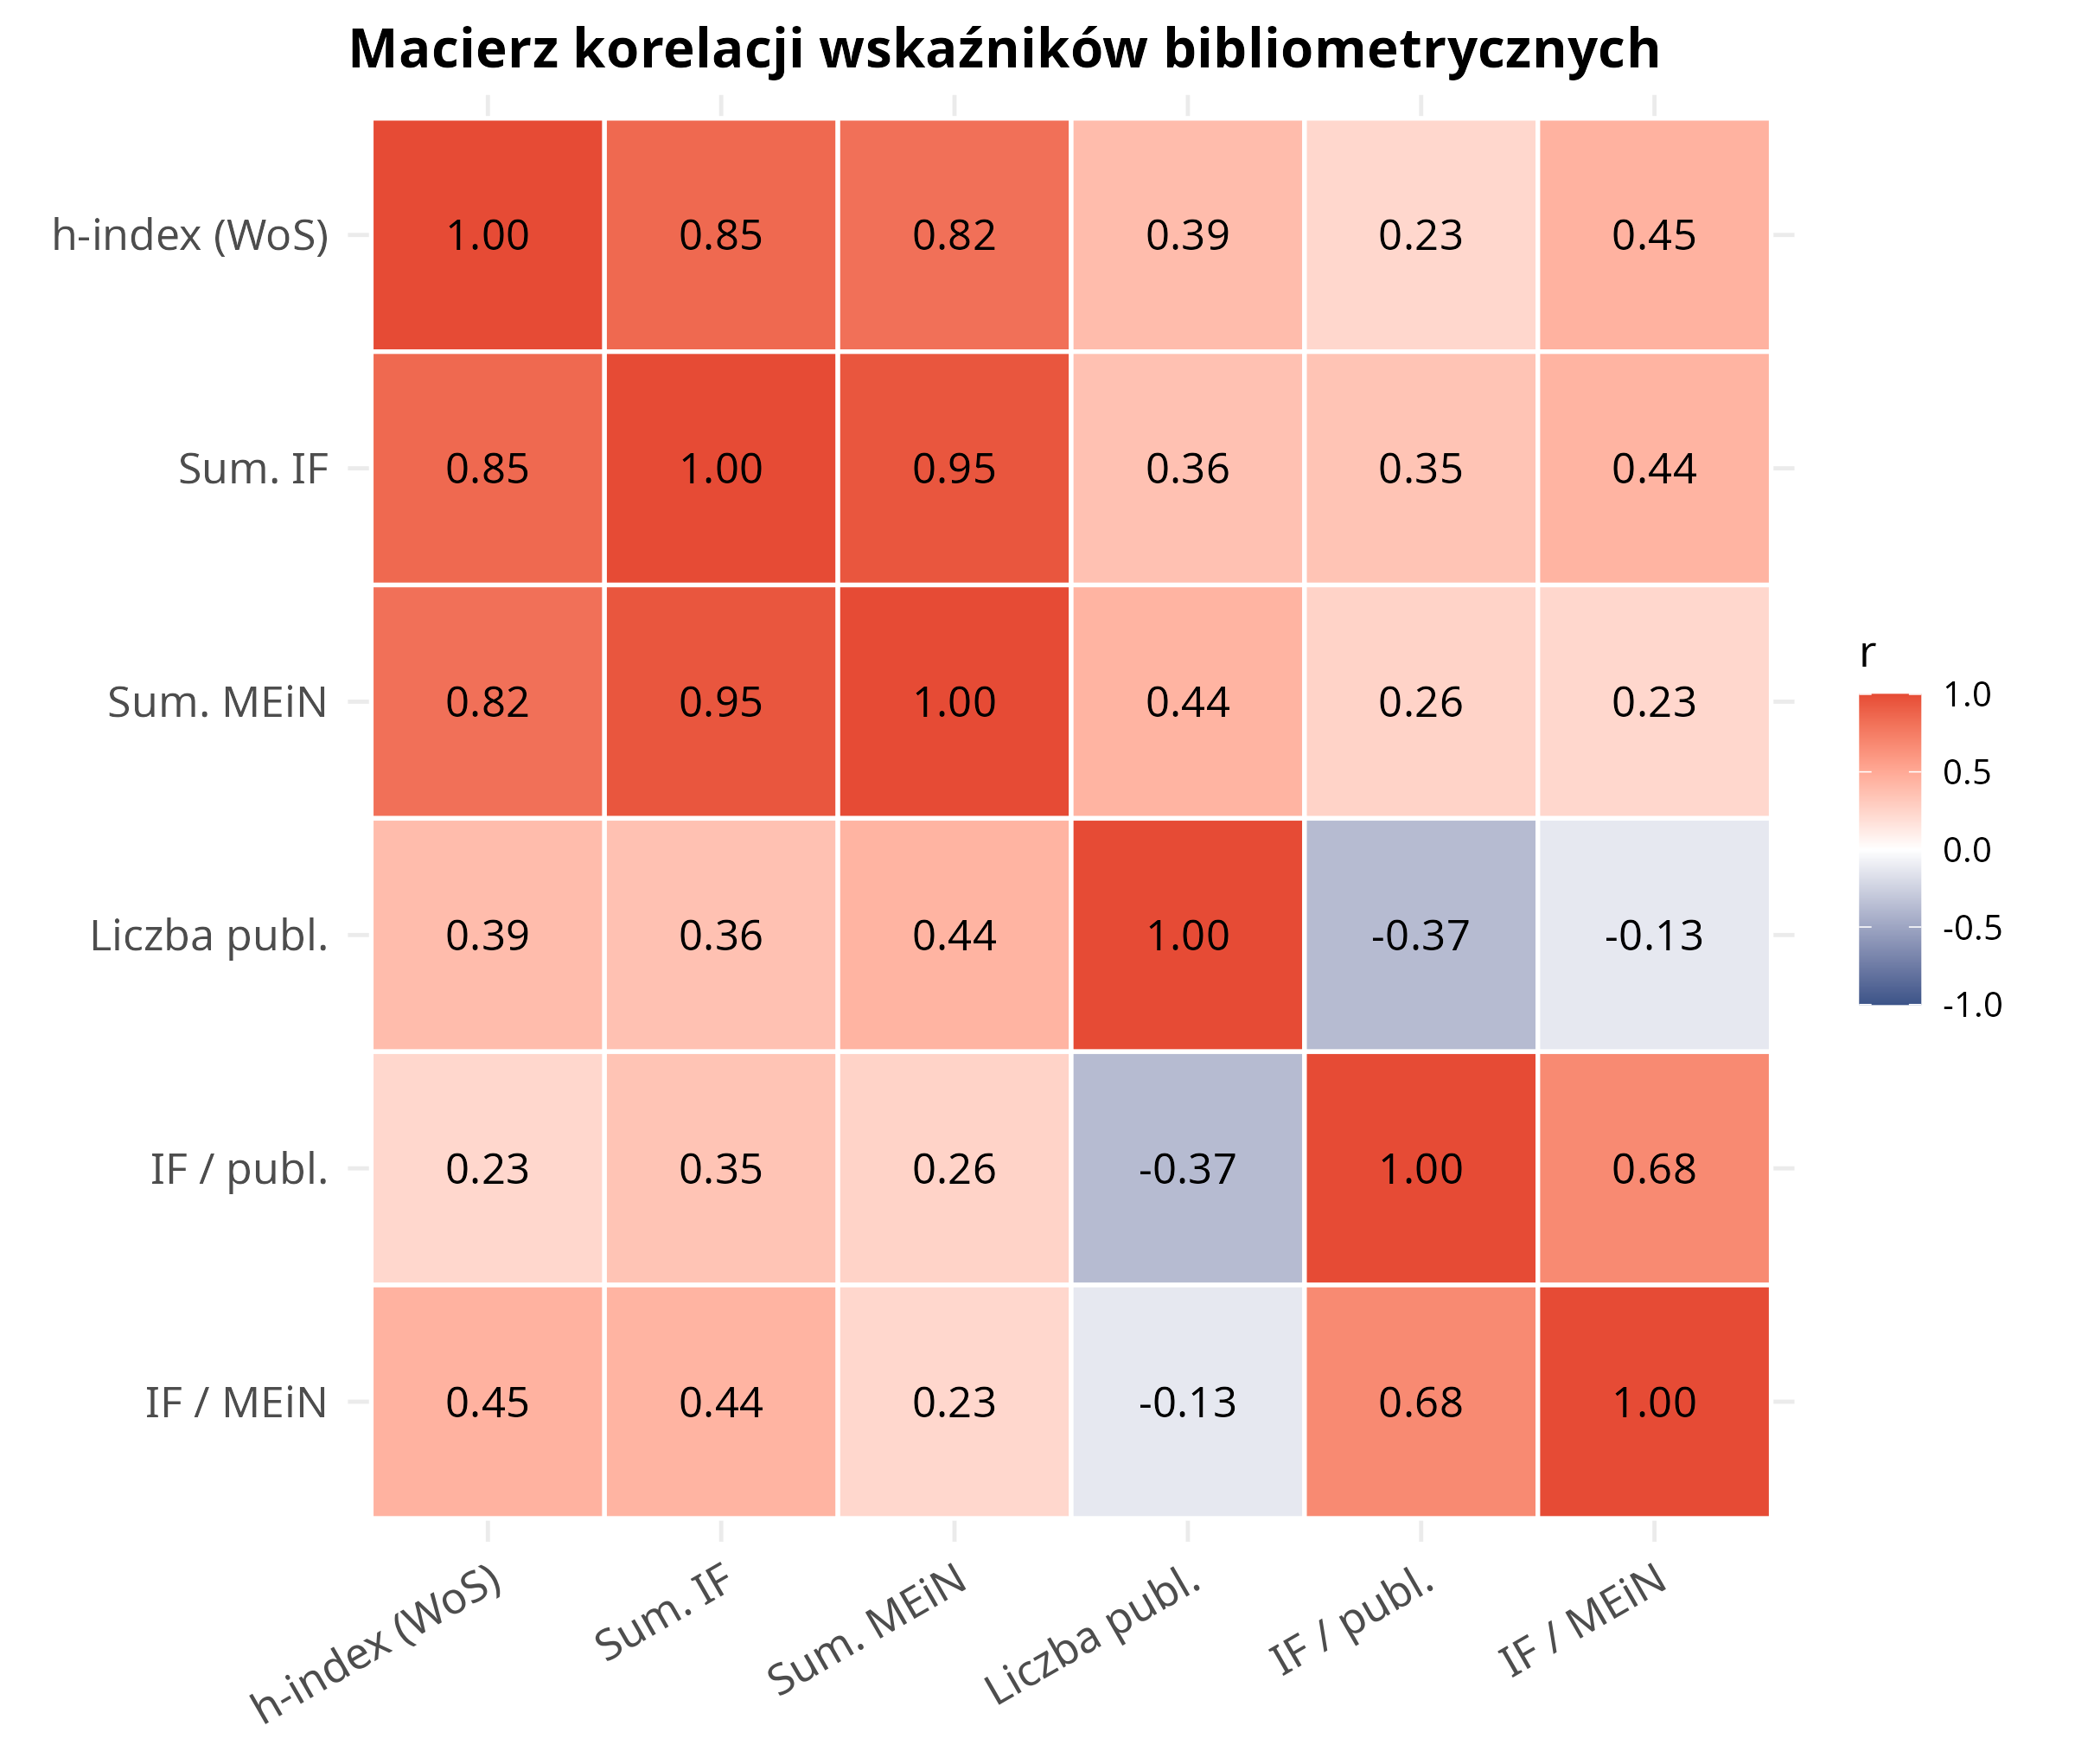
\includegraphics[width=1\linewidth,height=\textheight,keepaspectratio]{../Wykresy/praca/fig_01b_korelacje.png}

}

\caption{\label{fig-korelacje}Macierz korelacji Pearsona sześciu
wskaźników bibliometrycznych. Wyraźny blok metryk skumulowanego wpływu
(h-index, sumaryczny IF, punktacja MEiN; r 0,82--0,95) kontrastuje z
liczbą publikacji, powiązaną z nim tylko umiarkowanie (r 0,36--0,44),
oraz z IF na publikację, tworzącym odrębną oś jakości, ujemnie
skorelowaną z liczbą publikacji.}

\end{figure}%

\subsection{Różnice we wskaźnikach bibliometrycznych według uczelni i
stanowiska (pytanie
2)}\label{ruxf3ux17cnice-we-wskaux17anikach-bibliometrycznych-wedux142ug-uczelni-i-stanowiska-pytanie-2}

Dla sześciu analizowanych wskaźników sprawdzono, czy można zastosować
klasyczne testy parametryczne. Testy Shapiro-Wilka i Levene'a pokazały
jednak, że dane nie spełniają ich założeń: rozkłady nie są normalne, a
wariancje w grupach nie są równe. Z tego powodu zastosowano testy
nieparametryczne: test Kruskala-Wallisa oraz, w przypadku istotnych
różnic, test post-hoc Dunna z korektą Bonferroniego.

Decyzję tę uzasadnia także kształt rozkładów, który przedstawia
Rysunek~\ref{fig-rozklady}. Większość wskaźników bibliometrycznych ma
rozkłady silnie prawoskośne: wiele osób ma niskie lub umiarkowane
wartości, a niewielka grupa osiąga bardzo wysokie wyniki. Te wysokie
wartości odpowiadają jednak realnemu dorobkowi nielicznych, wybitnych
badaczy, a nie błędom w danych, dlatego nie usuwano ich jako wartości
odstających. Zastosowane testy rangowe są na takie skrajne obserwacje
odporne, więc analiza nie wymagała przycinania danych. Wyjątkiem jest
wskaźnik IF / MEiN, którego rozkład jest bardziej symetryczny, ale także
dla niego testy wykazały naruszenie założeń testów parametrycznych.

\begin{figure}[H]

\centering{

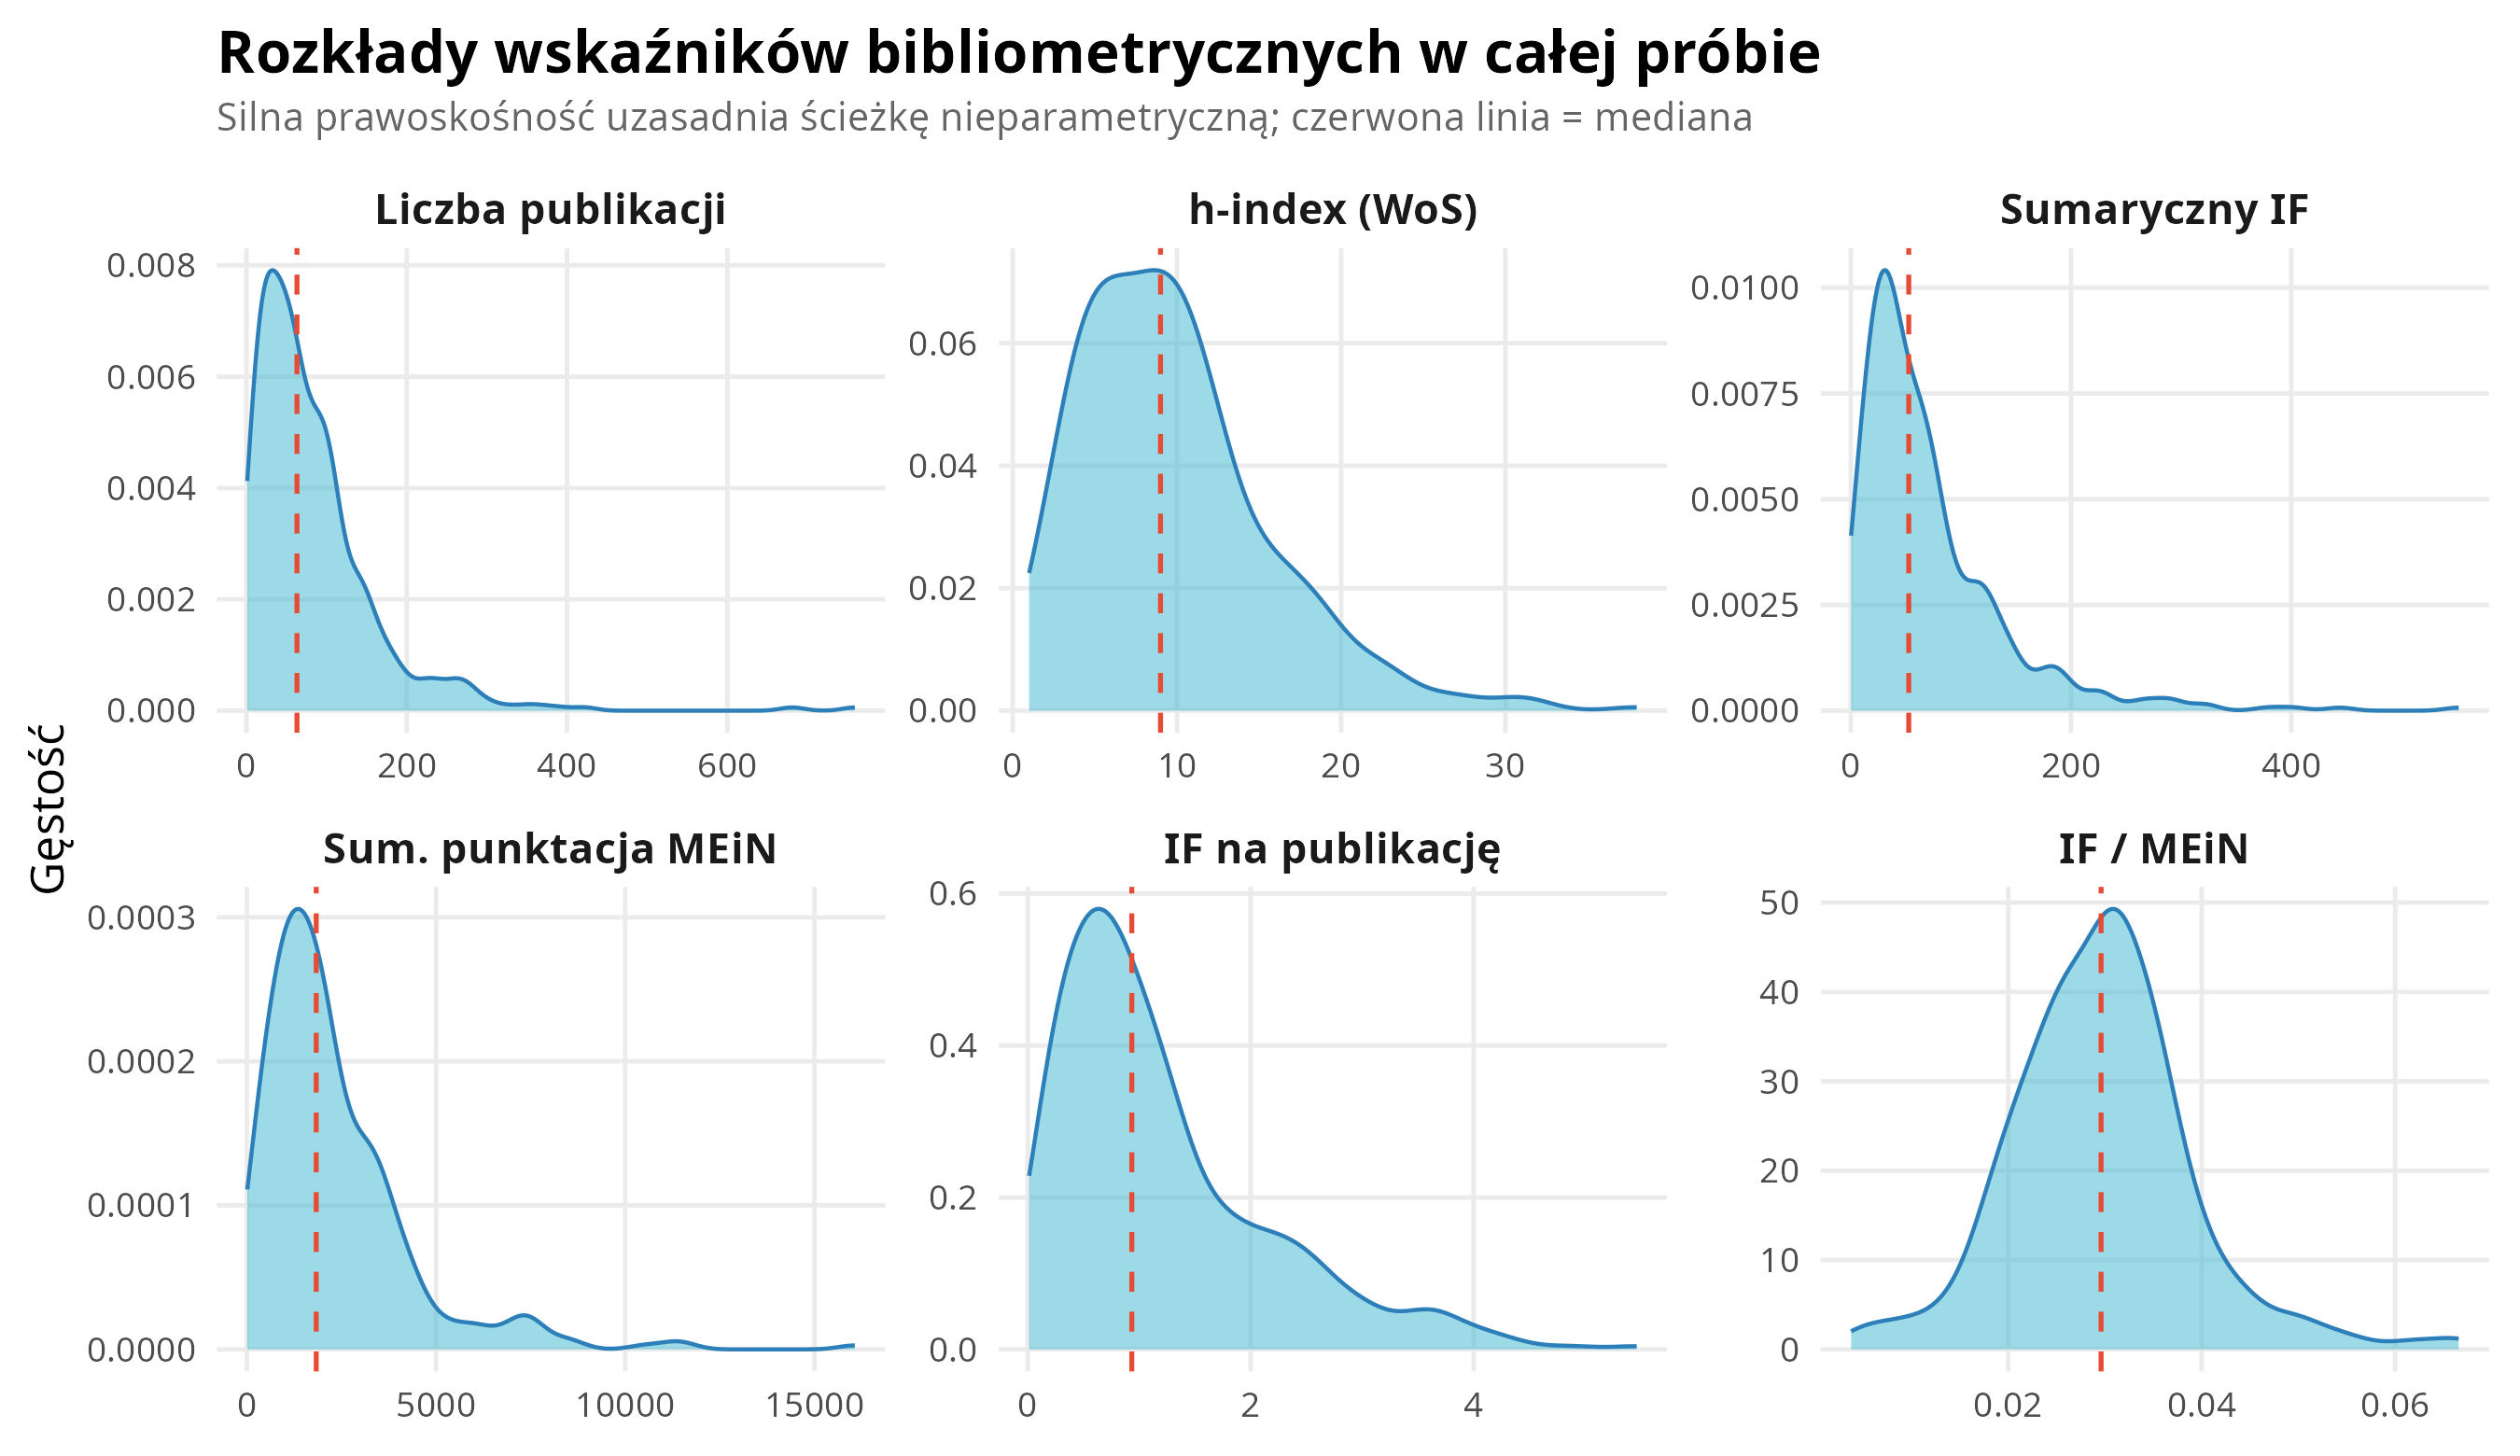
\includegraphics[width=1\linewidth,height=\textheight,keepaspectratio]{../Wykresy/praca/fig_01c_rozklady.png}

}

\caption{\label{fig-rozklady}Rozkłady (gęstości jądrowe) sześciu
wskaźników bibliometrycznych w całej próbie. Przewaga długich prawych
ogonów i położenie mediany (czerwona linia przerywana) poniżej średniej
potwierdzają silną prawoskośność, uzasadniającą wybór testów
nieparametrycznych.}

\end{figure}%

Wyniki tego porównania dla trzech metryk o pełnym pokryciu pokazano jako
wykresy pudełkowe z oznaczeniami grup jednorodnych
(Rysunek~\ref{fig-hindex}, Rysunek~\ref{fig-sumif},
Rysunek~\ref{fig-npub}). Na każdym z nich naniesiono dwa niezależne
zestawy grup jednorodnych (CLD): \textbf{małe niebieskie litery} nad
pudełkami porównują stanowiska w obrębie każdej uczelni, a \textbf{DUŻE
zielone litery} pod pudełkami porównują uczelnie w obrębie każdego
stanowiska (czyta się je, zestawiając pudełka tego samego koloru między
uczelniami); wspólna litera oznacza brak istotnej różnicy.

\begin{figure}[H]

\centering{

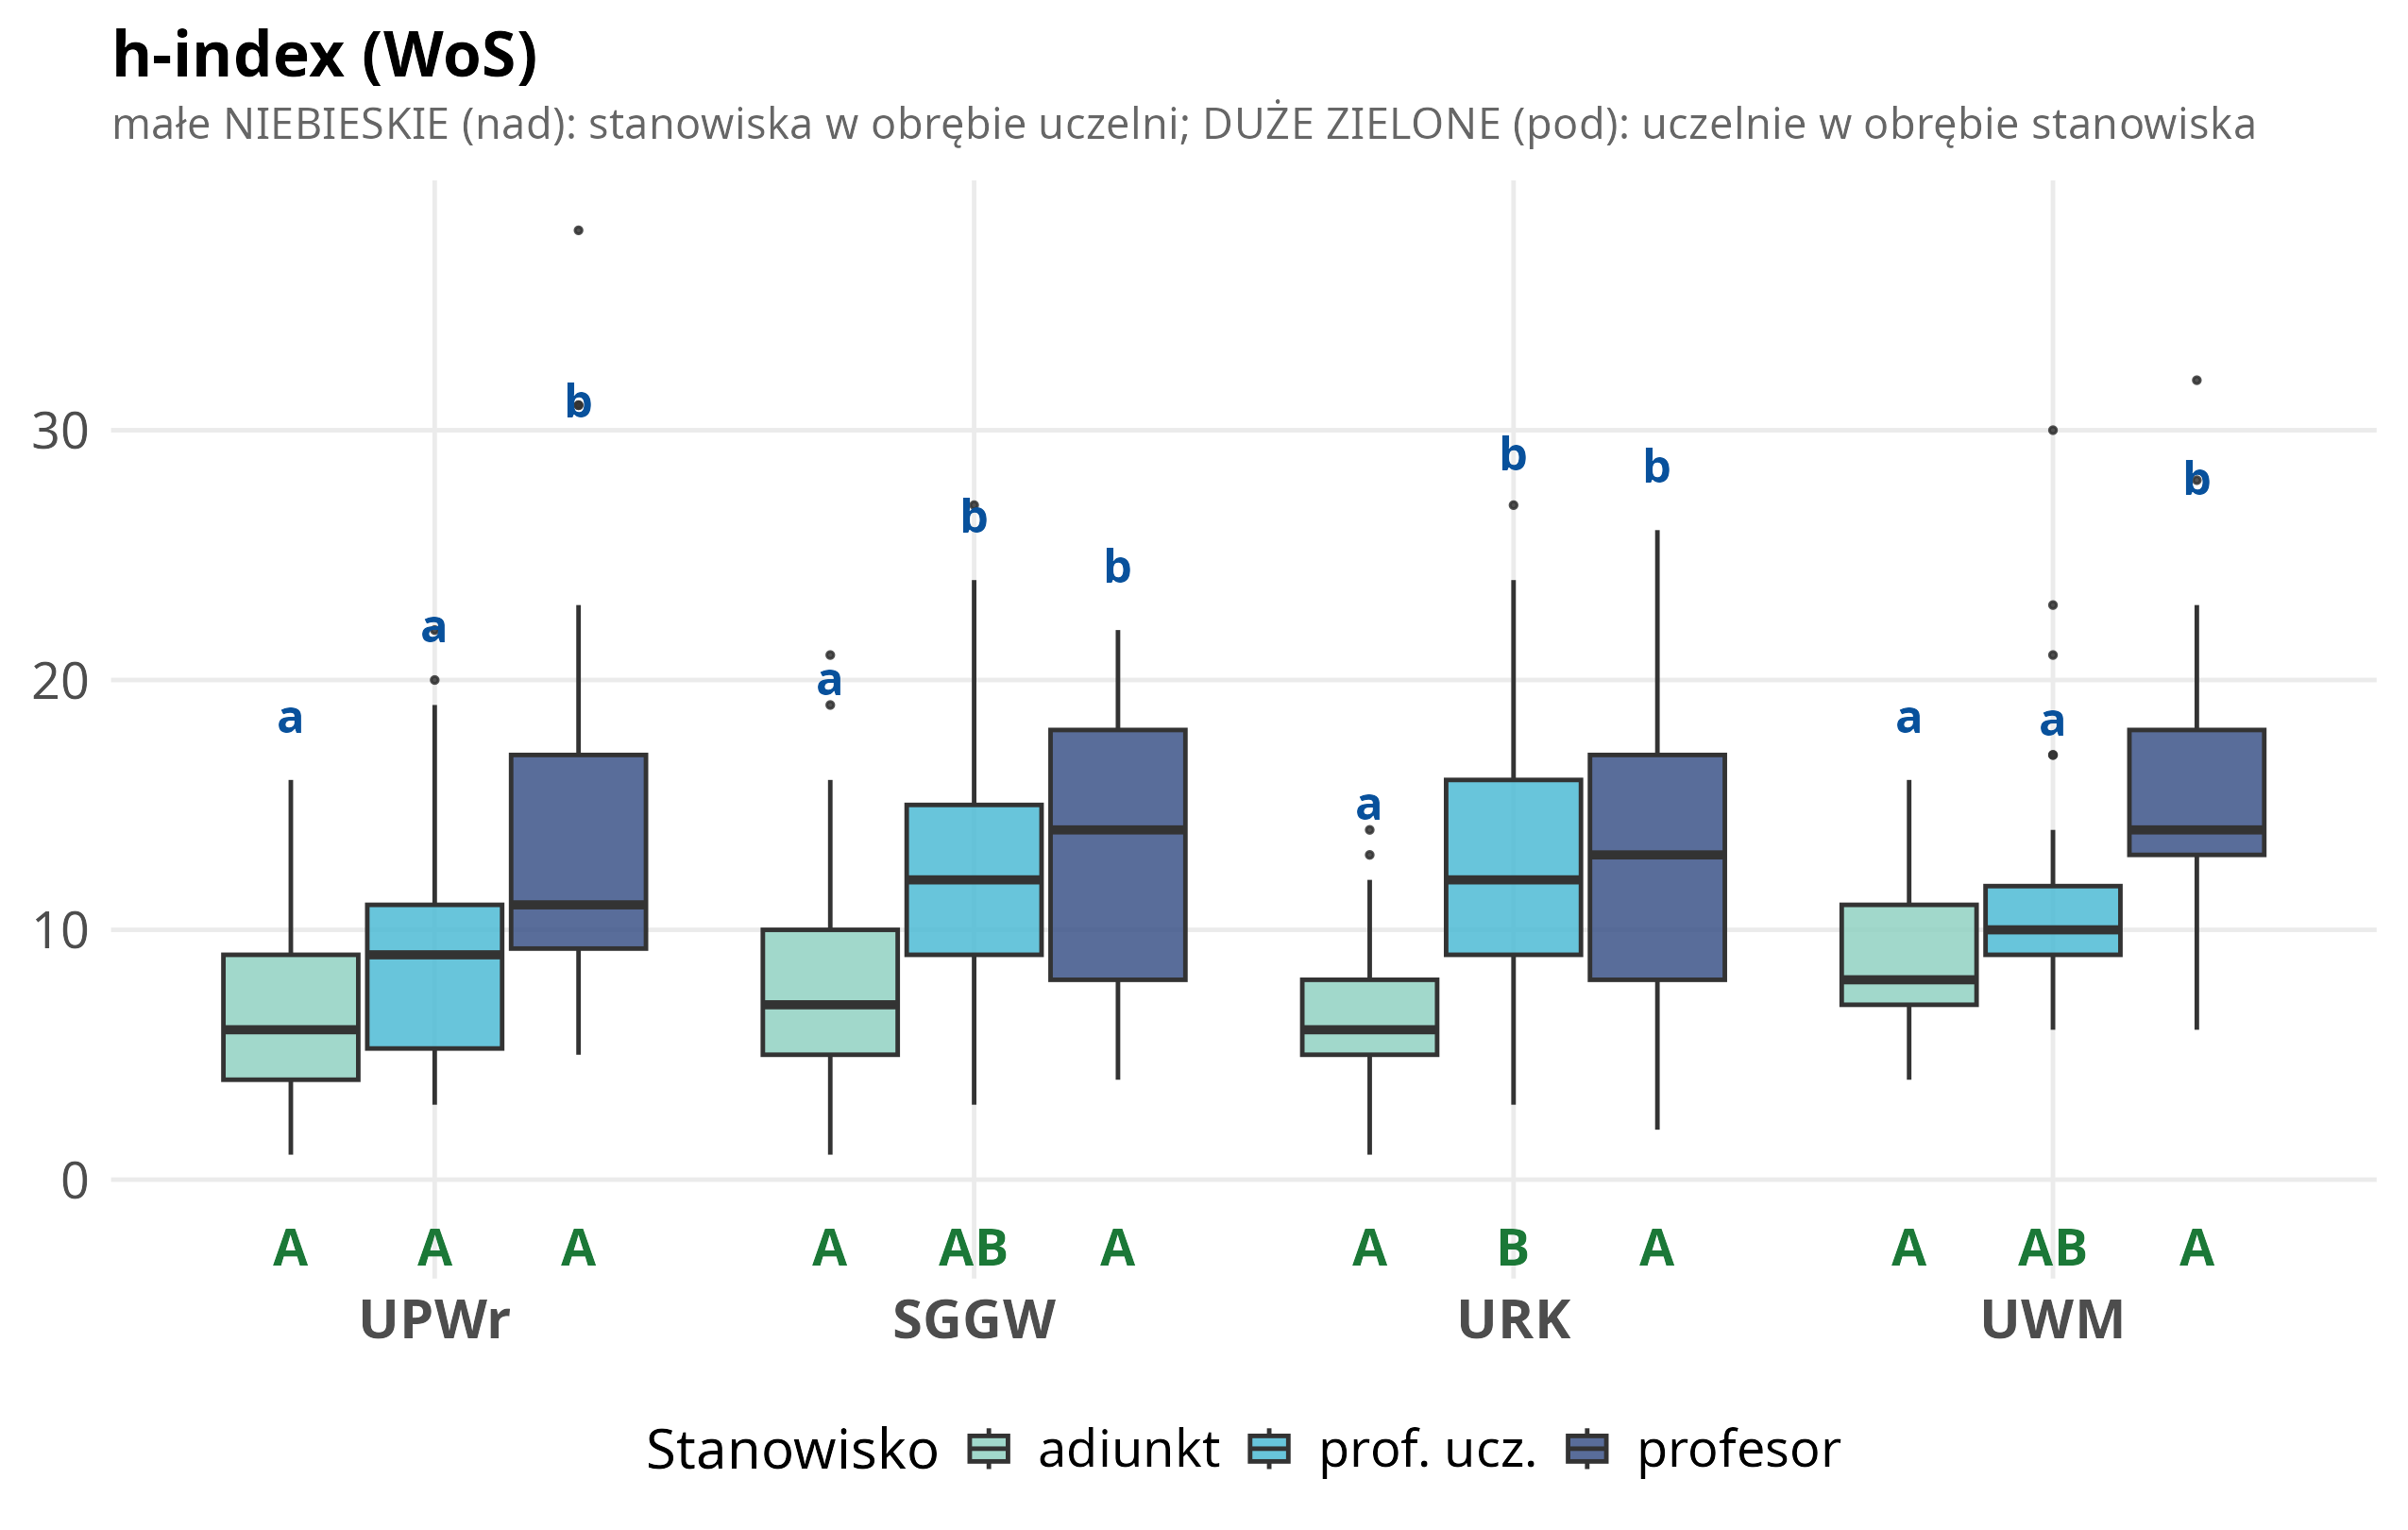
\includegraphics[width=1\linewidth,height=\textheight,keepaspectratio]{../Wykresy/praca/fig_02a_hindex.png}

}

\caption{\label{fig-hindex}Wykres pudełkowy h-index (WoS) w
dwuczynnikowym układzie uczelnia × stanowisko; oznaczenia grup
jednorodnych (CLD) opisano w tekście powyżej.}

\end{figure}%

\begin{figure}[H]

\centering{

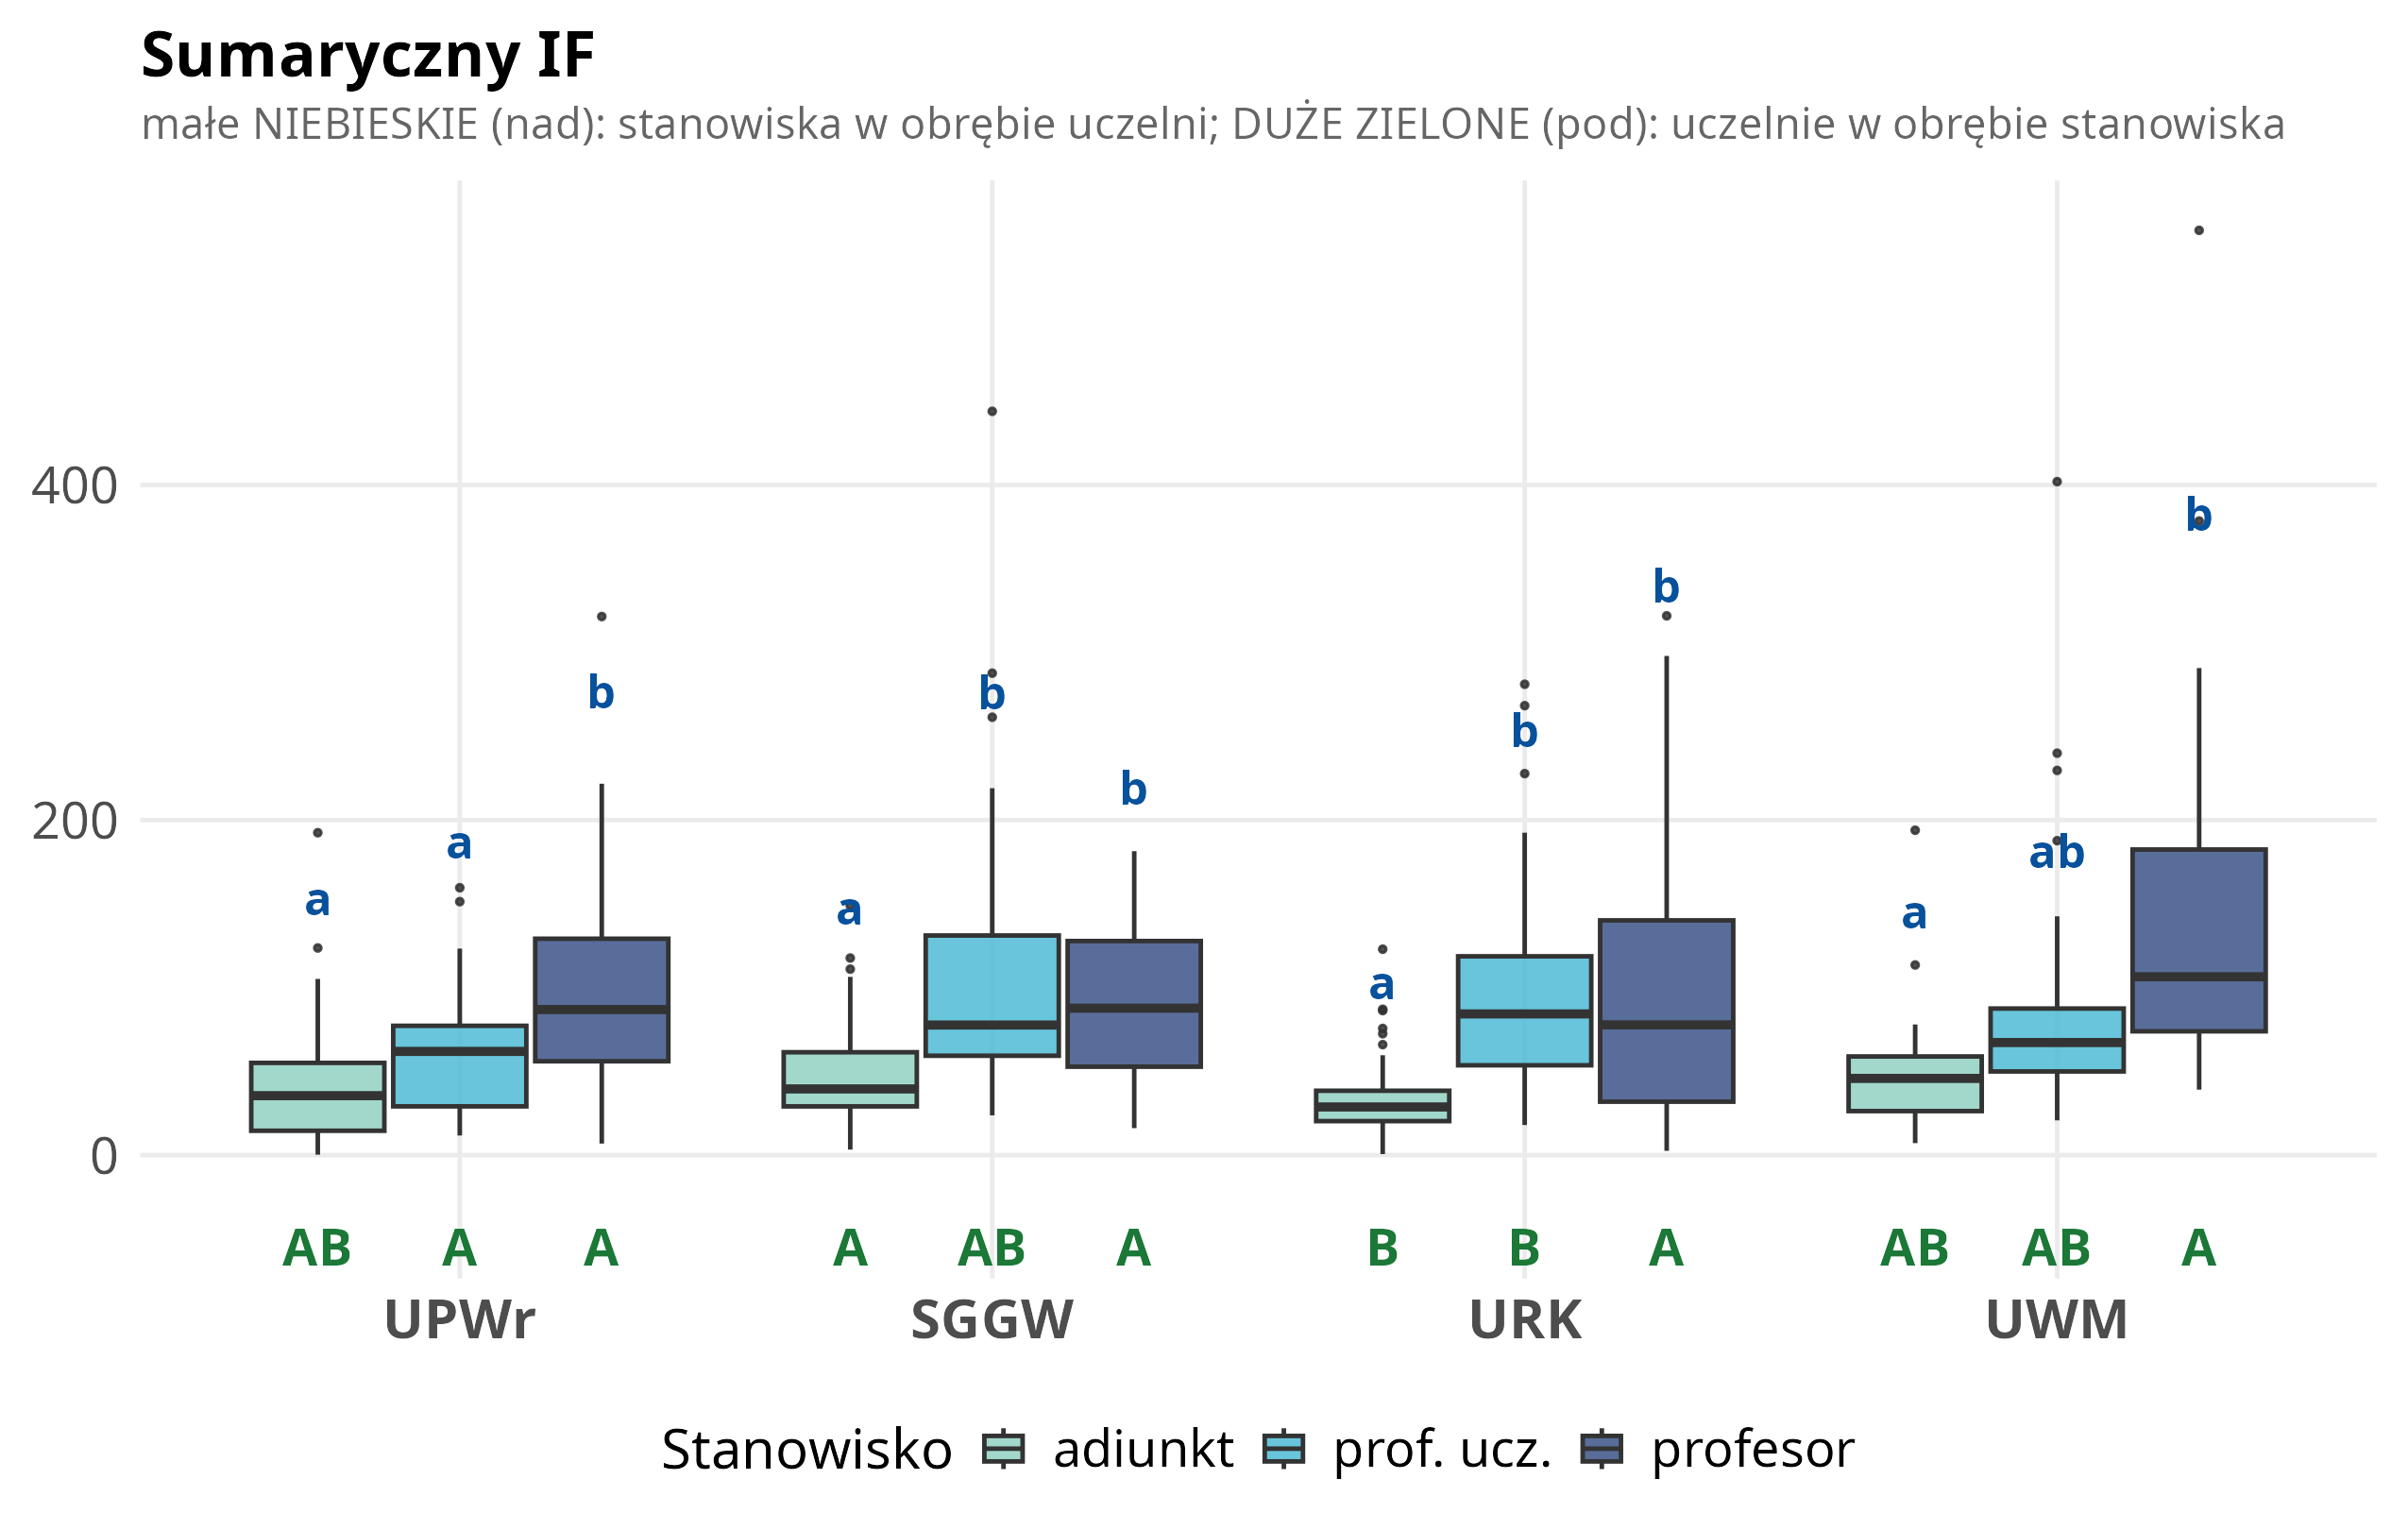
\includegraphics[width=1\linewidth,height=\textheight,keepaspectratio]{../Wykresy/praca/fig_02b_sumif.png}

}

\caption{\label{fig-sumif}Wykres pudełkowy sumarycznego Impact Factor w
dwuczynnikowym układzie uczelnia × stanowisko; oznaczenia grup
jednorodnych (CLD) opisano w tekście powyżej.}

\end{figure}%

\begin{figure}[H]

\centering{

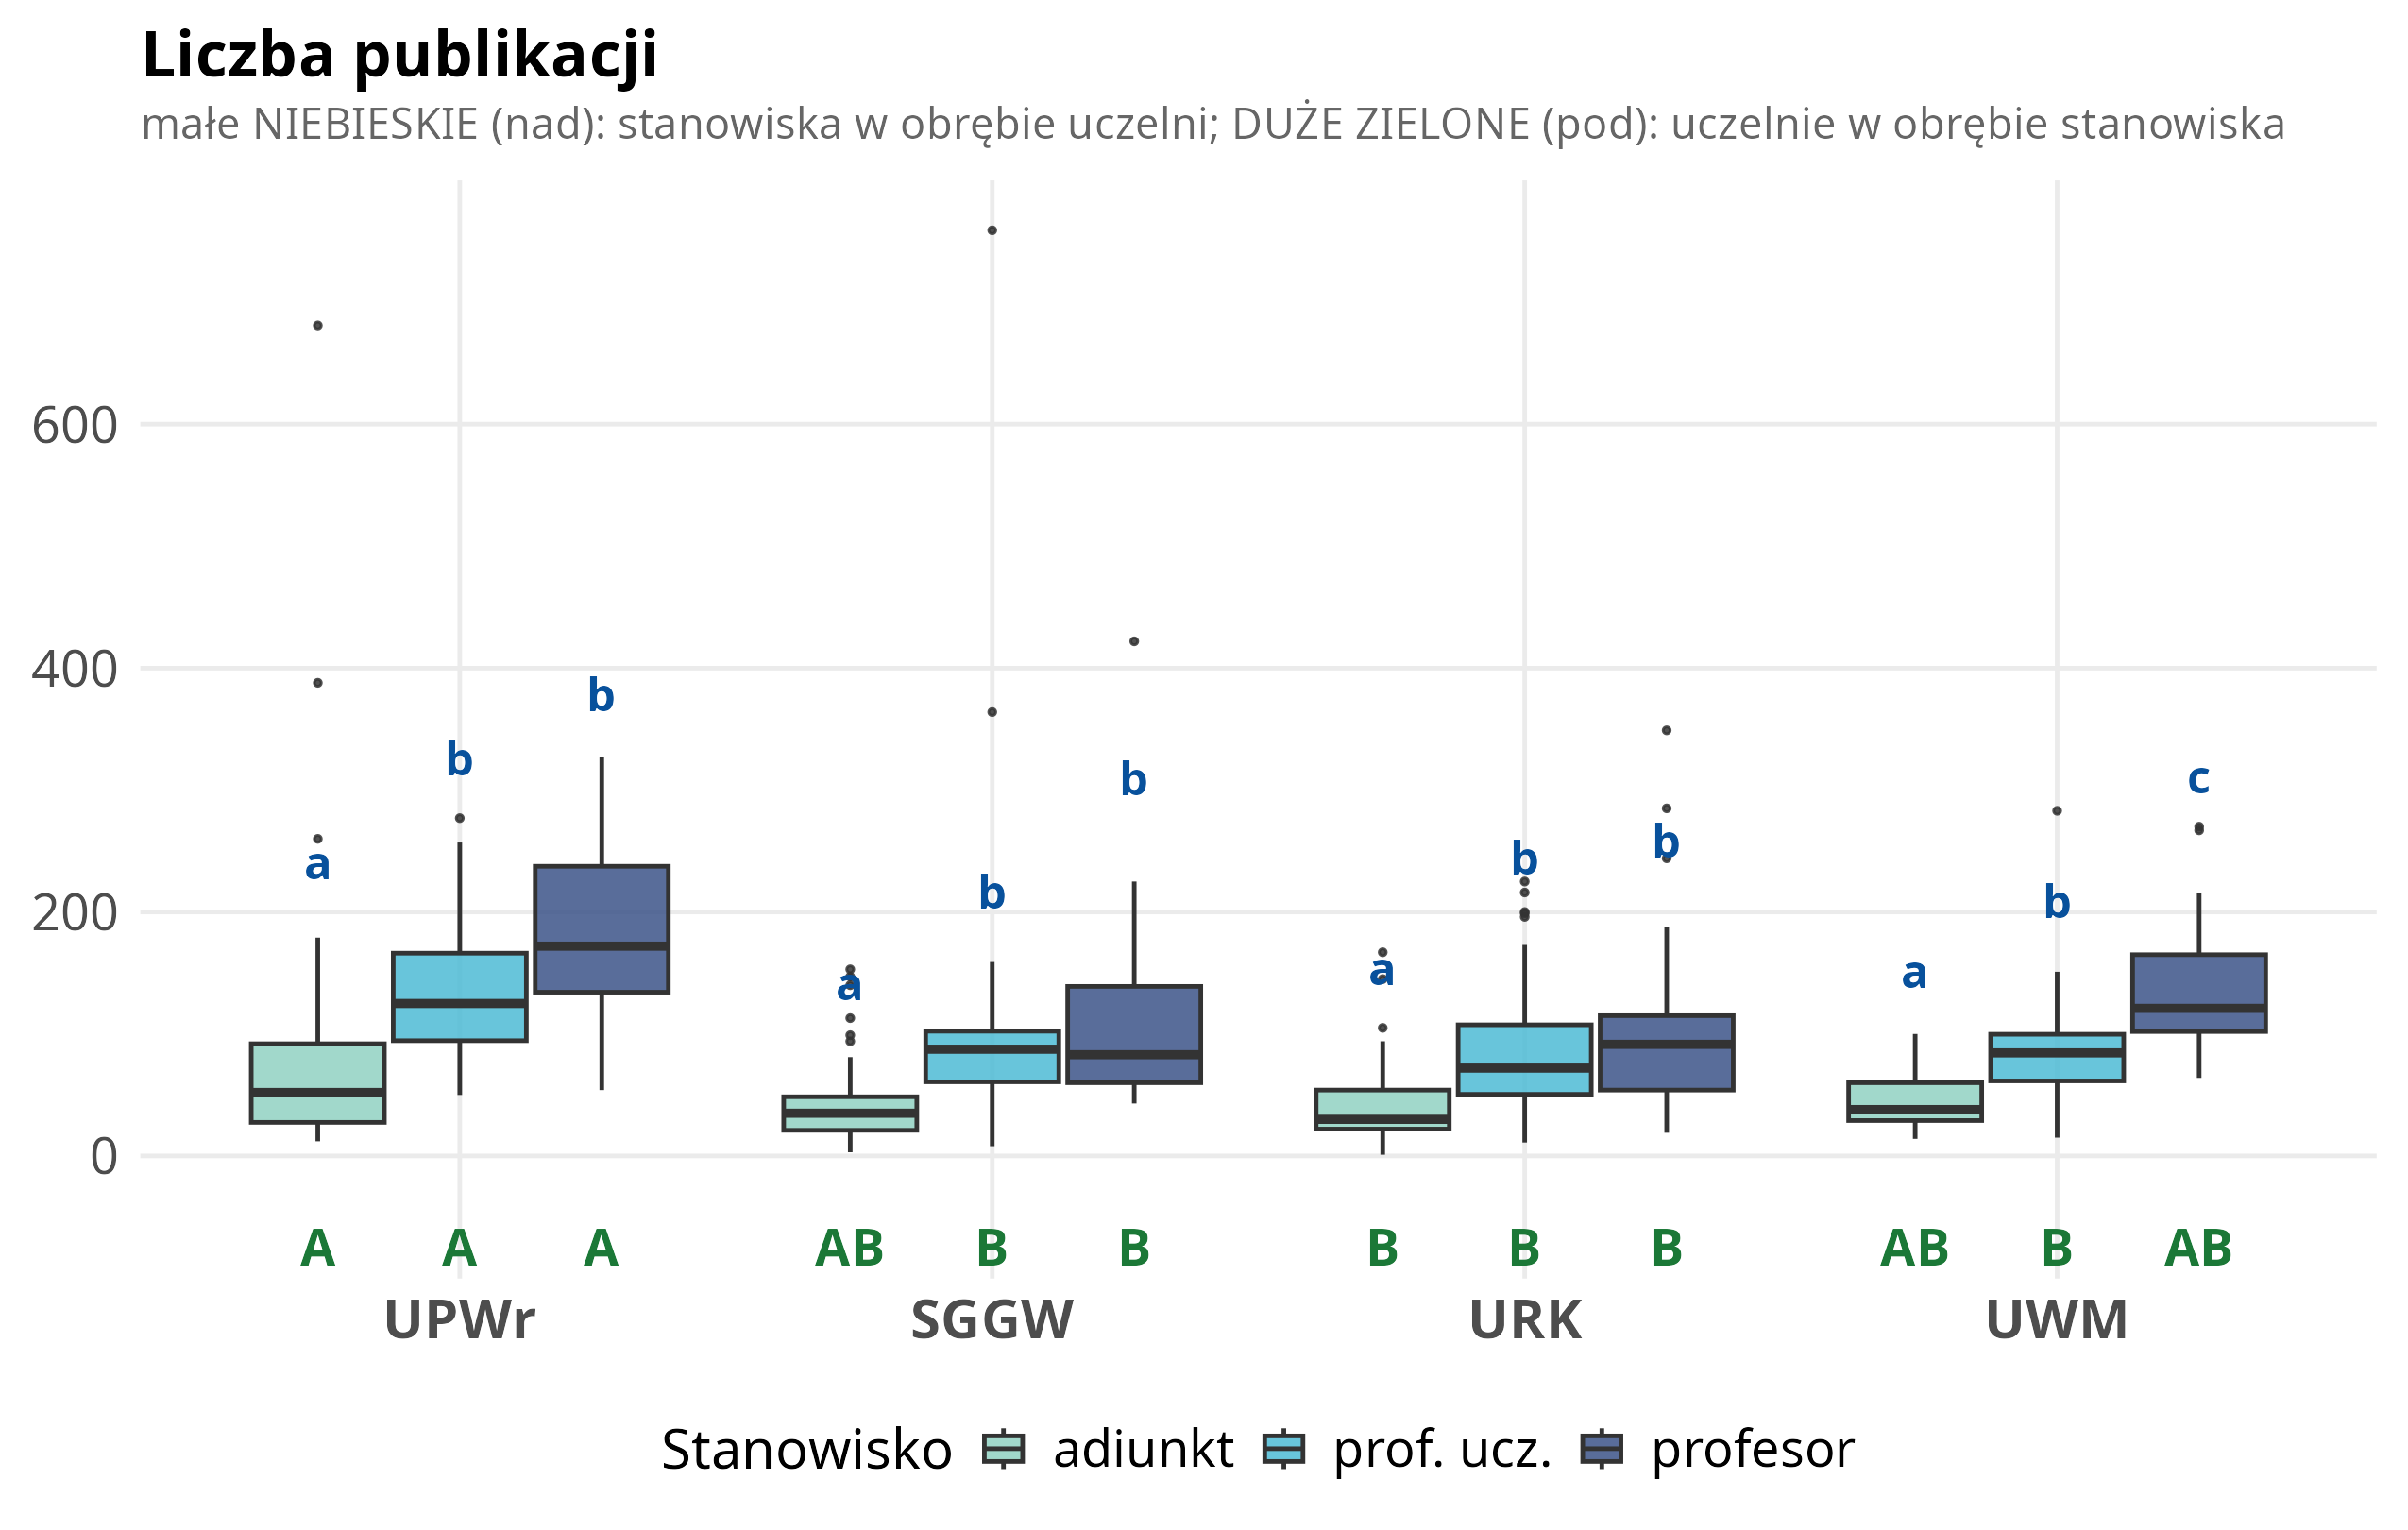
\includegraphics[width=1\linewidth,height=\textheight,keepaspectratio]{../Wykresy/praca/fig_02c_npub.png}

}

\caption{\label{fig-npub}Wykres pudełkowy liczby publikacji w
dwuczynnikowym układzie uczelnia × stanowisko; oznaczenia grup
jednorodnych (CLD) opisano w tekście powyżej.}

\end{figure}%

Wyniki pokazują, że wskaźniki bibliometryczne są silniej związane ze
stanowiskiem niż z uczelnią. We wszystkich czterech uczelniach widoczny
jest podobny układ: najniższe wartości mają adiunkci, wyższe
profesorowie uczelni, a najwyższe profesorowie.

Porównania post-hoc wykonane osobno w obrębie każdej uczelni pokazują,
że adiunkci najczęściej różnią się istotnie od obu grup profesorskich.
Natomiast profesorowie uczelni i profesorowie różnią się między sobą
rzadziej.

Porównania między uczelniami w obrębie tego samego stanowiska dają
słabsze różnice. Oznacza to, że osoby na podobnym stanowisku mają zwykle
podobne wskaźniki niezależnie od uczelni. Nieliczne różnice między
uczelniami dotyczą głównie liczby publikacji, która była najniższa w
UPWr.

Analizę przeprowadzono w dwóch krokach. Najpierw zastosowano test
Kruskala-Wallisa dla układu uczelnia × stanowisko, a następnie, tam
gdzie różnice były istotne, wykonano test post-hoc Dunna z korektą
Bonferroniego. Test ogólny był istotny dla pięciu z sześciu
analizowanych metryk. Jedynym wyjątkiem był wskaźnik IF / MEiN, dla
którego nie stwierdzono istotnych różnic (p = 0,075). Pełne wyniki
przedstawia Tabela~\ref{tbl-roznicowanie}.

\global\setlength{\Oldarrayrulewidth}{\arrayrulewidth}

\global\setlength{\Oldtabcolsep}{\tabcolsep}

\setlength{\tabcolsep}{2pt}

\renewcommand*{\arraystretch}{1.5}



\providecommand{\ascline}[3]{\noalign{\global\arrayrulewidth #1}\arrayrulecolor[HTML]{#2}\cline{#3}}

\begin{longtable}[c]{|p{1.85in}|p{0.95in}|p{0.85in}|p{1.10in}|p{1.05in}}

\caption{\label{tbl-roznicowanie}Ogólny test Kruskala-Wallisa i grupy
jednorodne z post-hoc (Dunn-Bonferroni) dla różnic w układzie uczelnia ×
stanowisko.}

\tabularnewline

\ascline{1.5pt}{666666}{1-5}

\multicolumn{1}{>{\centering}m{\dimexpr 1.85in+0\tabcolsep}}{\textcolor[HTML]{000000}{\fontsize{10}{10}\selectfont{\global\setmainfont{Latin Modern Roman}{Metryka}}}} & \multicolumn{1}{>{\centering}m{\dimexpr 0.95in+0\tabcolsep}}{\textcolor[HTML]{000000}{\fontsize{10}{10}\selectfont{\global\setmainfont{Latin Modern Roman}{H\ (df)*}}}} & \multicolumn{1}{>{\centering}m{\dimexpr 0.85in+0\tabcolsep}}{\textcolor[HTML]{000000}{\fontsize{10}{10}\selectfont{\global\setmainfont{Latin Modern Roman}{p\ (Kruskal-Wallis)}}}} & \multicolumn{1}{>{\centering}m{\dimexpr 1.1in+0\tabcolsep}}{\textcolor[HTML]{000000}{\fontsize{10}{10}\selectfont{\global\setmainfont{Latin Modern Roman}{Liczba\ grup\ CLD}}}} & \multicolumn{1}{>{\centering}m{\dimexpr 1.05in+0\tabcolsep}}{\textcolor[HTML]{000000}{\fontsize{10}{10}\selectfont{\global\setmainfont{Latin Modern Roman}{Istotność\ testu}}}} \\

\ascline{1.5pt}{666666}{1-5}\endfirsthead 

\ascline{1.5pt}{666666}{1-5}

\multicolumn{1}{>{\centering}m{\dimexpr 1.85in+0\tabcolsep}}{\textcolor[HTML]{000000}{\fontsize{10}{10}\selectfont{\global\setmainfont{Latin Modern Roman}{Metryka}}}} & \multicolumn{1}{>{\centering}m{\dimexpr 0.95in+0\tabcolsep}}{\textcolor[HTML]{000000}{\fontsize{10}{10}\selectfont{\global\setmainfont{Latin Modern Roman}{H\ (df)*}}}} & \multicolumn{1}{>{\centering}m{\dimexpr 0.85in+0\tabcolsep}}{\textcolor[HTML]{000000}{\fontsize{10}{10}\selectfont{\global\setmainfont{Latin Modern Roman}{p\ (Kruskal-Wallis)}}}} & \multicolumn{1}{>{\centering}m{\dimexpr 1.1in+0\tabcolsep}}{\textcolor[HTML]{000000}{\fontsize{10}{10}\selectfont{\global\setmainfont{Latin Modern Roman}{Liczba\ grup\ CLD}}}} & \multicolumn{1}{>{\centering}m{\dimexpr 1.05in+0\tabcolsep}}{\textcolor[HTML]{000000}{\fontsize{10}{10}\selectfont{\global\setmainfont{Latin Modern Roman}{Istotność\ testu}}}} \\

\ascline{1.5pt}{666666}{1-5}\endhead



\multicolumn{1}{>{\raggedright}m{\dimexpr 1.85in+0\tabcolsep}}{\textcolor[HTML]{000000}{\fontsize{10}{10}\selectfont{\global\setmainfont{Latin Modern Roman}{Liczba\ publikacji}}}} & \multicolumn{1}{>{\centering}m{\dimexpr 0.95in+0\tabcolsep}}{\textcolor[HTML]{000000}{\fontsize{10}{10}\selectfont{\global\setmainfont{Latin Modern Roman}{169,6\ (11)}}}} & \multicolumn{1}{>{\centering}m{\dimexpr 0.85in+0\tabcolsep}}{\textcolor[HTML]{000000}{\fontsize{10}{10}\selectfont{\global\setmainfont{Latin Modern Roman}{<\ 0,001}}}} & \multicolumn{1}{>{\centering}m{\dimexpr 1.1in+0\tabcolsep}}{\textcolor[HTML]{000000}{\fontsize{10}{10}\selectfont{\global\setmainfont{Latin Modern Roman}{8}}}} & \multicolumn{1}{>{\raggedright}m{\dimexpr 1.05in+0\tabcolsep}}{\textcolor[HTML]{000000}{\fontsize{10}{10}\selectfont{\global\setmainfont{Latin Modern Roman}{istotne}}}} \\





\multicolumn{1}{>{\raggedright}m{\dimexpr 1.85in+0\tabcolsep}}{\textcolor[HTML]{000000}{\fontsize{10}{10}\selectfont{\global\setmainfont{Latin Modern Roman}{IF\ na\ publikację}}}} & \multicolumn{1}{>{\centering}m{\dimexpr 0.95in+0\tabcolsep}}{\textcolor[HTML]{000000}{\fontsize{10}{10}\selectfont{\global\setmainfont{Latin Modern Roman}{54,7\ (11)}}}} & \multicolumn{1}{>{\centering}m{\dimexpr 0.85in+0\tabcolsep}}{\textcolor[HTML]{000000}{\fontsize{10}{10}\selectfont{\global\setmainfont{Latin Modern Roman}{<\ 0,001}}}} & \multicolumn{1}{>{\centering}m{\dimexpr 1.1in+0\tabcolsep}}{\textcolor[HTML]{000000}{\fontsize{10}{10}\selectfont{\global\setmainfont{Latin Modern Roman}{5}}}} & \multicolumn{1}{>{\raggedright}m{\dimexpr 1.05in+0\tabcolsep}}{\textcolor[HTML]{000000}{\fontsize{10}{10}\selectfont{\global\setmainfont{Latin Modern Roman}{istotne}}}} \\





\multicolumn{1}{>{\raggedright}m{\dimexpr 1.85in+0\tabcolsep}}{\textcolor[HTML]{000000}{\fontsize{10}{10}\selectfont{\global\setmainfont{Latin Modern Roman}{Sumaryczna\ punktacja\ MEiN\ (3\ uczelnie)}}}} & \multicolumn{1}{>{\centering}m{\dimexpr 0.95in+0\tabcolsep}}{\textcolor[HTML]{000000}{\fontsize{10}{10}\selectfont{\global\setmainfont{Latin Modern Roman}{108,6\ (8)}}}} & \multicolumn{1}{>{\centering}m{\dimexpr 0.85in+0\tabcolsep}}{\textcolor[HTML]{000000}{\fontsize{10}{10}\selectfont{\global\setmainfont{Latin Modern Roman}{<\ 0,001}}}} & \multicolumn{1}{>{\centering}m{\dimexpr 1.1in+0\tabcolsep}}{\textcolor[HTML]{000000}{\fontsize{10}{10}\selectfont{\global\setmainfont{Latin Modern Roman}{6}}}} & \multicolumn{1}{>{\raggedright}m{\dimexpr 1.05in+0\tabcolsep}}{\textcolor[HTML]{000000}{\fontsize{10}{10}\selectfont{\global\setmainfont{Latin Modern Roman}{istotne}}}} \\





\multicolumn{1}{>{\raggedright}m{\dimexpr 1.85in+0\tabcolsep}}{\textcolor[HTML]{000000}{\fontsize{10}{10}\selectfont{\global\setmainfont{Latin Modern Roman}{h-index\ (WoS)}}}} & \multicolumn{1}{>{\centering}m{\dimexpr 0.95in+0\tabcolsep}}{\textcolor[HTML]{000000}{\fontsize{10}{10}\selectfont{\global\setmainfont{Latin Modern Roman}{118,6\ (11)}}}} & \multicolumn{1}{>{\centering}m{\dimexpr 0.85in+0\tabcolsep}}{\textcolor[HTML]{000000}{\fontsize{10}{10}\selectfont{\global\setmainfont{Latin Modern Roman}{<\ 0,001}}}} & \multicolumn{1}{>{\centering}m{\dimexpr 1.1in+0\tabcolsep}}{\textcolor[HTML]{000000}{\fontsize{10}{10}\selectfont{\global\setmainfont{Latin Modern Roman}{6}}}} & \multicolumn{1}{>{\raggedright}m{\dimexpr 1.05in+0\tabcolsep}}{\textcolor[HTML]{000000}{\fontsize{10}{10}\selectfont{\global\setmainfont{Latin Modern Roman}{istotne}}}} \\





\multicolumn{1}{>{\raggedright}m{\dimexpr 1.85in+0\tabcolsep}}{\textcolor[HTML]{000000}{\fontsize{10}{10}\selectfont{\global\setmainfont{Latin Modern Roman}{Sumaryczny\ IF}}}} & \multicolumn{1}{>{\centering}m{\dimexpr 0.95in+0\tabcolsep}}{\textcolor[HTML]{000000}{\fontsize{10}{10}\selectfont{\global\setmainfont{Latin Modern Roman}{108,8\ (11)}}}} & \multicolumn{1}{>{\centering}m{\dimexpr 0.85in+0\tabcolsep}}{\textcolor[HTML]{000000}{\fontsize{10}{10}\selectfont{\global\setmainfont{Latin Modern Roman}{<\ 0,001}}}} & \multicolumn{1}{>{\centering}m{\dimexpr 1.1in+0\tabcolsep}}{\textcolor[HTML]{000000}{\fontsize{10}{10}\selectfont{\global\setmainfont{Latin Modern Roman}{6}}}} & \multicolumn{1}{>{\raggedright}m{\dimexpr 1.05in+0\tabcolsep}}{\textcolor[HTML]{000000}{\fontsize{10}{10}\selectfont{\global\setmainfont{Latin Modern Roman}{istotne}}}} \\





\multicolumn{1}{>{\raggedright}m{\dimexpr 1.85in+0\tabcolsep}}{\textcolor[HTML]{000000}{\fontsize{10}{10}\selectfont{\global\setmainfont{Latin Modern Roman}{IF\ /\ MEiN}}}} & \multicolumn{1}{>{\centering}m{\dimexpr 0.95in+0\tabcolsep}}{\textcolor[HTML]{000000}{\fontsize{10}{10}\selectfont{\global\setmainfont{Latin Modern Roman}{14,3\ (8)}}}} & \multicolumn{1}{>{\centering}m{\dimexpr 0.85in+0\tabcolsep}}{\textcolor[HTML]{000000}{\fontsize{10}{10}\selectfont{\global\setmainfont{Latin Modern Roman}{0,075}}}} & \multicolumn{1}{>{\centering}m{\dimexpr 1.1in+0\tabcolsep}}{\textcolor[HTML]{000000}{\fontsize{10}{10}\selectfont{\global\setmainfont{Latin Modern Roman}{1}}}} & \multicolumn{1}{>{\raggedright}m{\dimexpr 1.05in+0\tabcolsep}}{\textcolor[HTML]{000000}{\fontsize{10}{10}\selectfont{\global\setmainfont{Latin Modern Roman}{brak\ różnic}}}} \\

\ascline{1.5pt}{666666}{1-5}



\multicolumn{5}{>{\raggedright}m{\dimexpr 5.8in+8\tabcolsep}}{\textcolor[HTML]{000000}{\fontsize{9}{9}\selectfont{\global\setmainfont{Latin Modern Roman}{*\ H\ to\ statystyka\ Kruskala-Wallisa\ (rozkład\ chi-kwadrat\ o\ df\ stopniach\ swobody).}}}} \\




\end{longtable}

\arrayrulecolor[HTML]{000000}

\global\setlength{\arrayrulewidth}{\Oldarrayrulewidth}

\global\setlength{\tabcolsep}{\Oldtabcolsep}

\renewcommand*{\arraystretch}{1}

Najwięcej różnic między grupami widać dla liczby publikacji. Ta metryka
podzieliła badanych na 8 grup jednorodnych, czyli najlepiej odróżniała
poszczególne kombinacje uczelni i stanowiska. Wyraźne różnice wystąpiły
także dla h-index, sumarycznego IF i punktacji MEiN.

Jedynym wskaźnikiem, dla którego nie stwierdzono istotnych różnic, był
IF / MEiN (p = 0,075). Wynika to z jego konstrukcji: jako iloraz dwóch
silnie skorelowanych wielkości znosi on efekt skali dorobku, więc nie
różnicuje wyraźnie badanych grup.

Podsumowując, wraz z wyższym stanowiskiem rosną wartości większości
wskaźników bibliometrycznych. Zależność ta była istotna statystycznie
dla pięciu z sześciu analizowanych metryk.

\subsection{Typy profili bibliometrycznych badaczy (pytanie
1)}\label{typy-profili-bibliometrycznych-badaczy-pytanie-1}

Analizę przeprowadzono na \textbf{połączonej próbie wszystkich czterech
uczelni}, na czterech porównywalnych, standaryzowanych cechach pełnego
pokrycia: h-index WoS, sumarycznym IF, IF na publikację i liczbie
publikacji. Objęła ona 449 osób (te spośród 462, dla których dostępny
był komplet czterech cech). Dwie pierwsze składowe PCA opisywały łącznie
\textbf{87,9 \% wariancji} (PC1: 54,1 \%, PC2: 33,8 \%), więc dobrze
streszczały główne różnice między profilami badaczy.

Liczbę klastrów dobrano metodą sylwetki. Metoda ta sprawdza, czy osoby w
danym klastrze są do siebie podobne i jednocześnie wyraźnie różnią się
od osób z innych klastrów. Najlepszy wynik uzyskał podział na
\textbf{dwa klastry} (Rysunek~\ref{fig-klastry}).

\begin{figure}[H]

\centering{

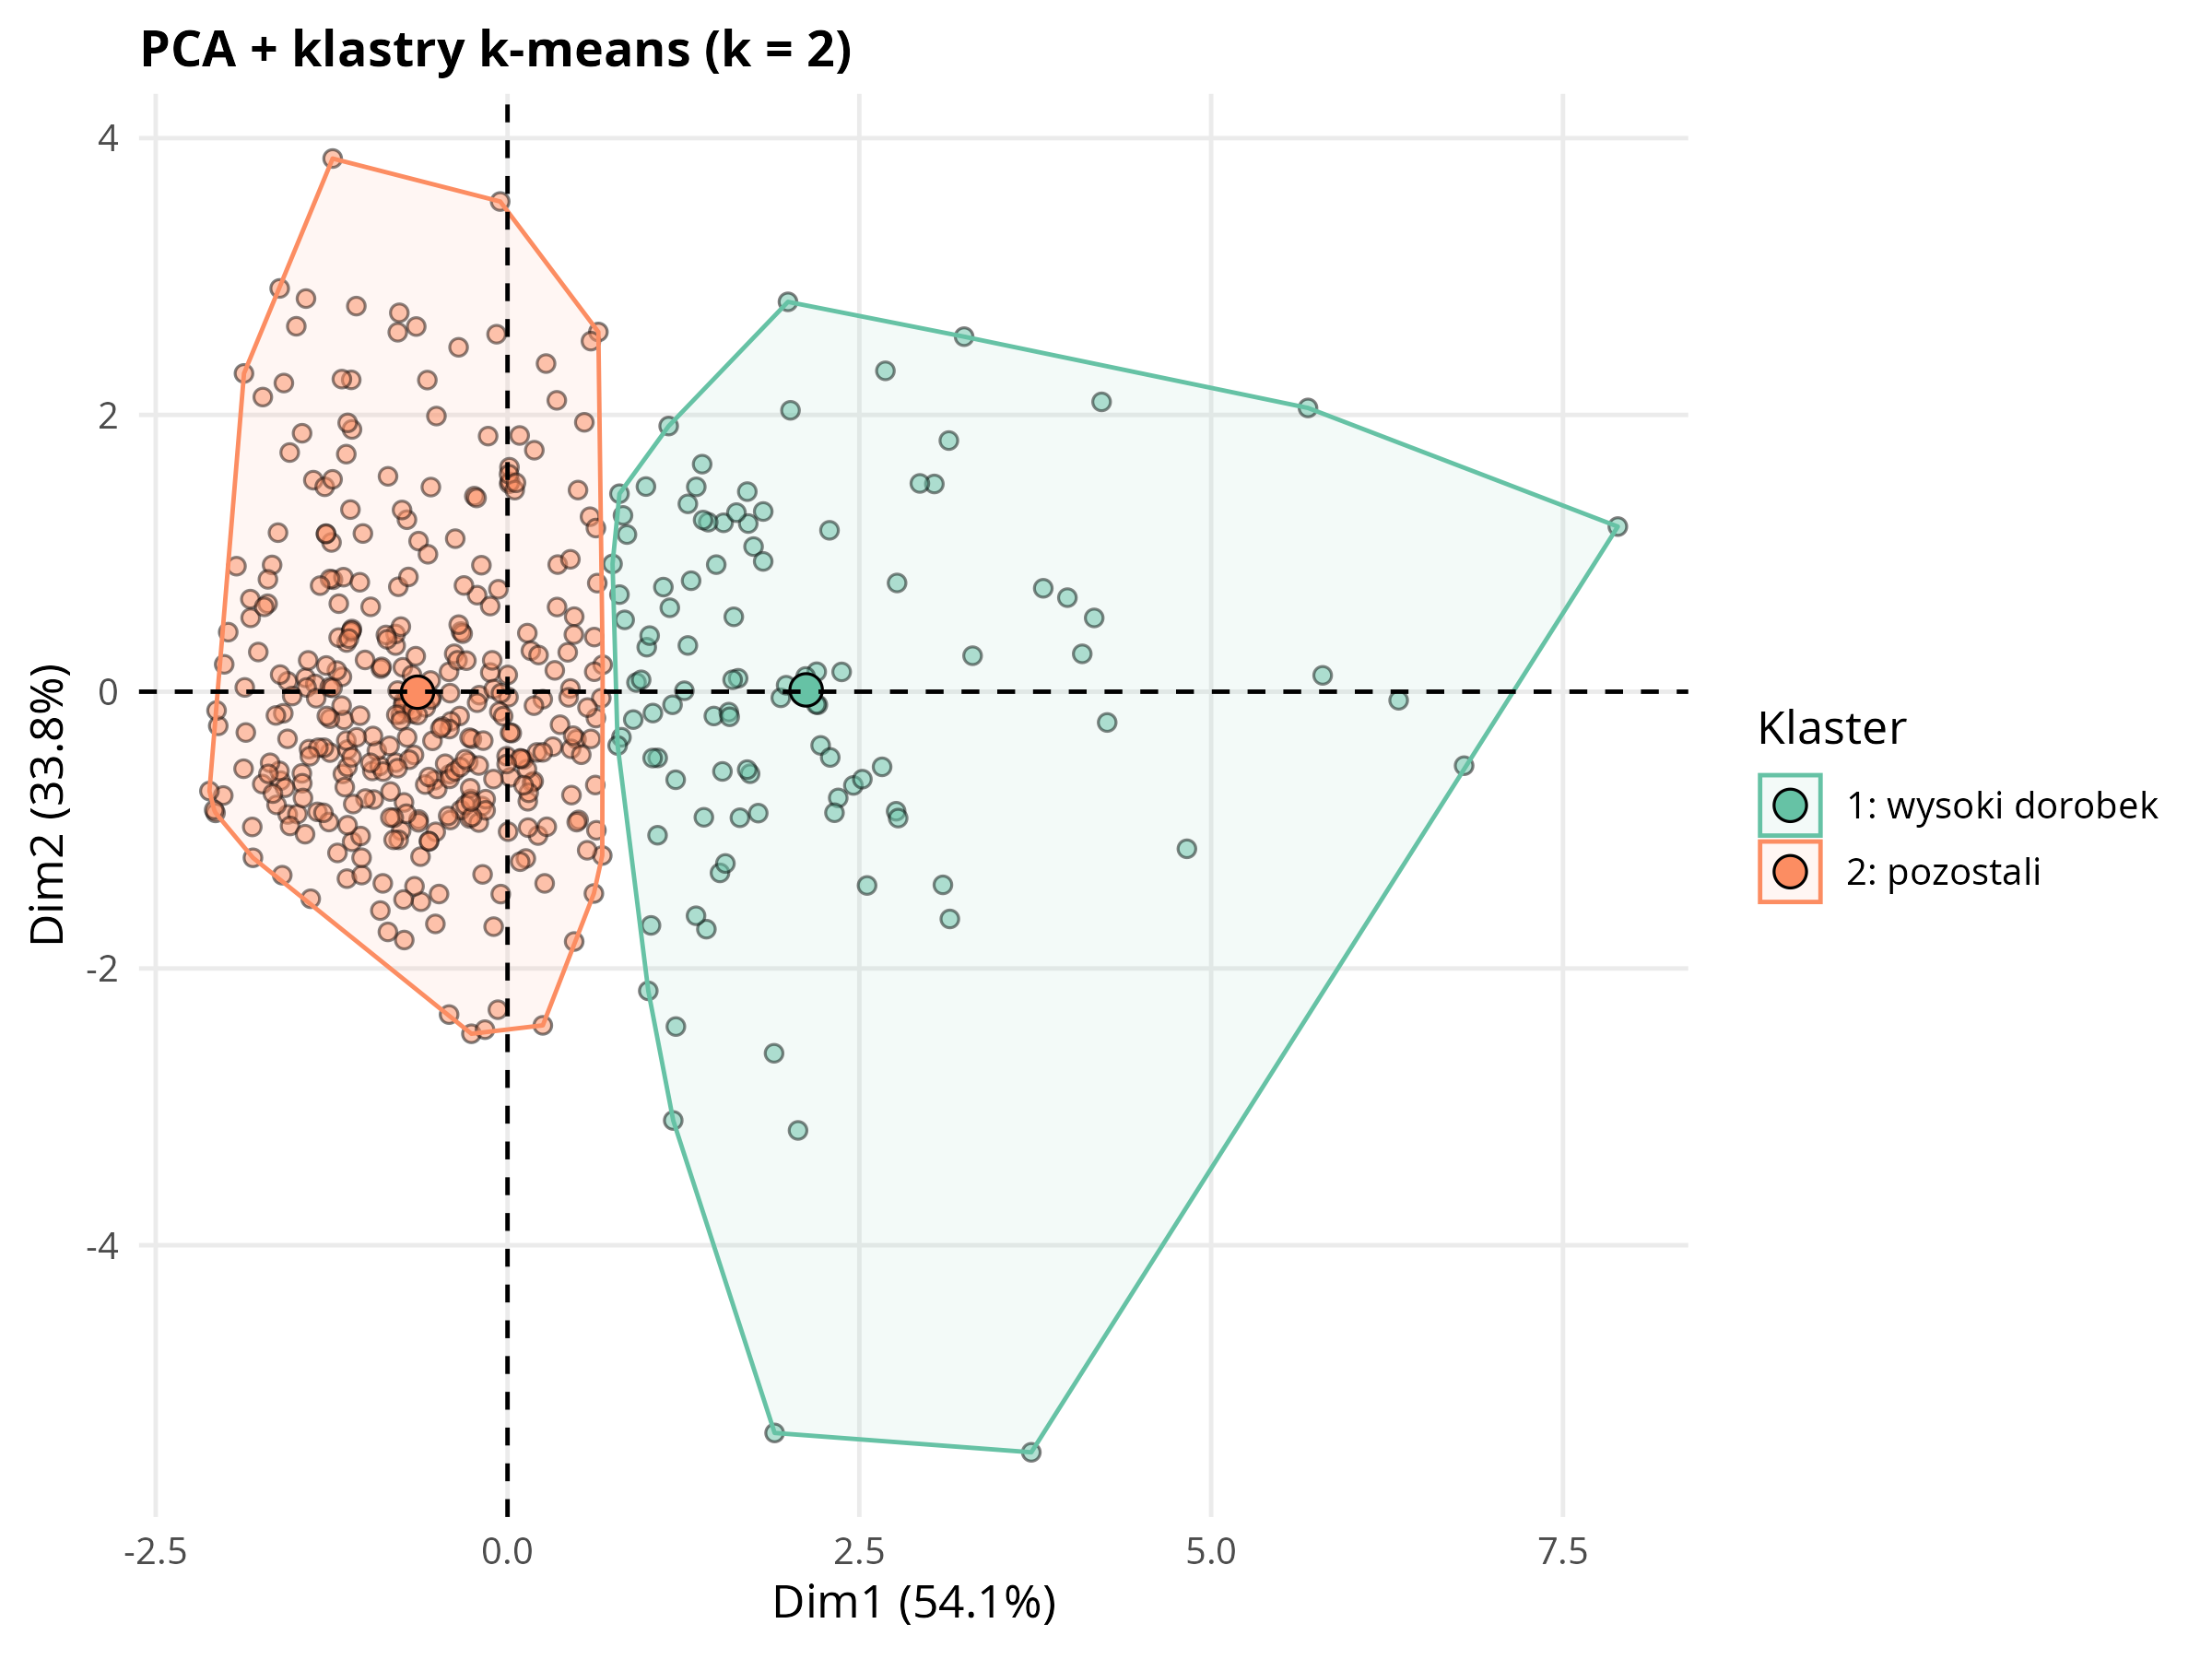
\includegraphics[width=1\linewidth,height=\textheight,keepaspectratio]{../Wykresy/praca/fig_03a_klastry.png}

}

\caption{\label{fig-klastry}Klastrowanie k-means w przestrzeni dwóch
pierwszych składowych głównych (PCA).}

\end{figure}%

Otrzymane klastry mają jednoznaczną interpretację jako podział na
\textbf{rdzeń wysokoproduktywny} i \textbf{pozostałą populację}
(Tabela~\ref{tbl-klastry2}):

\global\setlength{\Oldarrayrulewidth}{\arrayrulewidth}

\global\setlength{\Oldtabcolsep}{\tabcolsep}

\setlength{\tabcolsep}{2pt}

\renewcommand*{\arraystretch}{1.5}



\providecommand{\ascline}[3]{\noalign{\global\arrayrulewidth #1}\arrayrulecolor[HTML]{#2}\cline{#3}}

\begin{longtable}[c]{|p{1.55in}|p{0.50in}|p{0.95in}|p{1.05in}|p{1.05in}|p{1.05in}}

\caption{\label{tbl-klastry2}Średnie metryki dwóch klastrów k-means
(rozwiązanie główne).}

\tabularnewline

\ascline{1.5pt}{666666}{1-6}

\multicolumn{1}{>{\centering}m{\dimexpr 1.55in+0\tabcolsep}}{\textcolor[HTML]{000000}{\fontsize{10}{10}\selectfont{\global\setmainfont{Latin Modern Roman}{Klaster}}}} & \multicolumn{1}{>{\centering}m{\dimexpr 0.5in+0\tabcolsep}}{\textcolor[HTML]{000000}{\fontsize{10}{10}\selectfont{\global\setmainfont{Latin Modern Roman}{n}}}} & \multicolumn{1}{>{\centering}m{\dimexpr 0.95in+0\tabcolsep}}{\textcolor[HTML]{000000}{\fontsize{10}{10}\selectfont{\global\setmainfont{Latin Modern Roman}{h-index\ WoS}}}} & \multicolumn{1}{>{\centering}m{\dimexpr 1.05in+0\tabcolsep}}{\textcolor[HTML]{000000}{\fontsize{10}{10}\selectfont{\global\setmainfont{Latin Modern Roman}{Sumaryczny\ IF}}}} & \multicolumn{1}{>{\centering}m{\dimexpr 1.05in+0\tabcolsep}}{\textcolor[HTML]{000000}{\fontsize{10}{10}\selectfont{\global\setmainfont{Latin Modern Roman}{IF\ /\ publikację}}}} & \multicolumn{1}{>{\centering}m{\dimexpr 1.05in+0\tabcolsep}}{\textcolor[HTML]{000000}{\fontsize{10}{10}\selectfont{\global\setmainfont{Latin Modern Roman}{Liczba\ publikacji}}}} \\

\ascline{1.5pt}{666666}{1-6}\endfirsthead 

\ascline{1.5pt}{666666}{1-6}

\multicolumn{1}{>{\centering}m{\dimexpr 1.55in+0\tabcolsep}}{\textcolor[HTML]{000000}{\fontsize{10}{10}\selectfont{\global\setmainfont{Latin Modern Roman}{Klaster}}}} & \multicolumn{1}{>{\centering}m{\dimexpr 0.5in+0\tabcolsep}}{\textcolor[HTML]{000000}{\fontsize{10}{10}\selectfont{\global\setmainfont{Latin Modern Roman}{n}}}} & \multicolumn{1}{>{\centering}m{\dimexpr 0.95in+0\tabcolsep}}{\textcolor[HTML]{000000}{\fontsize{10}{10}\selectfont{\global\setmainfont{Latin Modern Roman}{h-index\ WoS}}}} & \multicolumn{1}{>{\centering}m{\dimexpr 1.05in+0\tabcolsep}}{\textcolor[HTML]{000000}{\fontsize{10}{10}\selectfont{\global\setmainfont{Latin Modern Roman}{Sumaryczny\ IF}}}} & \multicolumn{1}{>{\centering}m{\dimexpr 1.05in+0\tabcolsep}}{\textcolor[HTML]{000000}{\fontsize{10}{10}\selectfont{\global\setmainfont{Latin Modern Roman}{IF\ /\ publikację}}}} & \multicolumn{1}{>{\centering}m{\dimexpr 1.05in+0\tabcolsep}}{\textcolor[HTML]{000000}{\fontsize{10}{10}\selectfont{\global\setmainfont{Latin Modern Roman}{Liczba\ publikacji}}}} \\

\ascline{1.5pt}{666666}{1-6}\endhead



\multicolumn{1}{>{\raggedright}m{\dimexpr 1.55in+0\tabcolsep}}{\textcolor[HTML]{000000}{\fontsize{10}{10}\selectfont{\global\setmainfont{Latin Modern Roman}{1:\ wysoki\ dorobek}}}} & \multicolumn{1}{>{\centering}m{\dimexpr 0.5in+0\tabcolsep}}{\textcolor[HTML]{000000}{\fontsize{10}{10}\selectfont{\global\setmainfont{Latin Modern Roman}{104}}}} & \multicolumn{1}{>{\centering}m{\dimexpr 0.95in+0\tabcolsep}}{\textcolor[HTML]{000000}{\fontsize{10}{10}\selectfont{\global\setmainfont{Latin Modern Roman}{17,8}}}} & \multicolumn{1}{>{\centering}m{\dimexpr 1.05in+0\tabcolsep}}{\textcolor[HTML]{000000}{\fontsize{10}{10}\selectfont{\global\setmainfont{Latin Modern Roman}{163,1}}}} & \multicolumn{1}{>{\centering}m{\dimexpr 1.05in+0\tabcolsep}}{\textcolor[HTML]{000000}{\fontsize{10}{10}\selectfont{\global\setmainfont{Latin Modern Roman}{1,38}}}} & \multicolumn{1}{>{\centering}m{\dimexpr 1.05in+0\tabcolsep}}{\textcolor[HTML]{000000}{\fontsize{10}{10}\selectfont{\global\setmainfont{Latin Modern Roman}{160,7}}}} \\





\multicolumn{1}{>{\raggedright}m{\dimexpr 1.55in+0\tabcolsep}}{\textcolor[HTML]{000000}{\fontsize{10}{10}\selectfont{\global\setmainfont{Latin Modern Roman}{2:\ pozostali}}}} & \multicolumn{1}{>{\centering}m{\dimexpr 0.5in+0\tabcolsep}}{\textcolor[HTML]{000000}{\fontsize{10}{10}\selectfont{\global\setmainfont{Latin Modern Roman}{345}}}} & \multicolumn{1}{>{\centering}m{\dimexpr 0.95in+0\tabcolsep}}{\textcolor[HTML]{000000}{\fontsize{10}{10}\selectfont{\global\setmainfont{Latin Modern Roman}{7,4}}}} & \multicolumn{1}{>{\centering}m{\dimexpr 1.05in+0\tabcolsep}}{\textcolor[HTML]{000000}{\fontsize{10}{10}\selectfont{\global\setmainfont{Latin Modern Roman}{44,8}}}} & \multicolumn{1}{>{\centering}m{\dimexpr 1.05in+0\tabcolsep}}{\textcolor[HTML]{000000}{\fontsize{10}{10}\selectfont{\global\setmainfont{Latin Modern Roman}{1,17}}}} & \multicolumn{1}{>{\centering}m{\dimexpr 1.05in+0\tabcolsep}}{\textcolor[HTML]{000000}{\fontsize{10}{10}\selectfont{\global\setmainfont{Latin Modern Roman}{61,8}}}} \\

\ascline{1.5pt}{666666}{1-6}


\end{longtable}

\arrayrulecolor[HTML]{000000}

\global\setlength{\arrayrulewidth}{\Oldarrayrulewidth}

\global\setlength{\tabcolsep}{\Oldtabcolsep}

\renewcommand*{\arraystretch}{1}

Sprawdzono też, z czym wiąże się przynależność do klastrów, co
rozstrzyga, czy typologia jest cechą uczelni, czy etapu kariery: klastry
\textbf{nie zależą istotnie od uczelni} (χ² niezależności p = 0,19;
Craméra V = 0,10), ale są \textbf{wyraźnie powiązane ze stanowiskiem}
naukowym (p \textless{} 0,001; Craméra V = 0,45).

Oznacza to, że podział badaczy nie wynika głównie z tego, na której
uczelni pracują; bardziej odzwierciedla etap kariery i poziom dorobku
naukowego. Zbliżony układ profili bibliometrycznych powtarza się więc w
czterech uczelniach (z zastrzeżeniami omówionymi niżej przy replikacji w
obrębie pojedynczych uczelni).

Dodatkowo porównano wynik k-means z klastrowaniem hierarchicznym metodą
Warda. Zgodność obu metod była umiarkowana (Craméra V = 0,67), ale
główny podział na dwie duże grupy był podobny w obu podejściach.

W celu oceny, czy uzyskana typologia nie wynika wyłącznie z połączenia
wszystkich uczelni w jedną próbę, klastrowanie powtórzono osobno dla
każdej uczelni. W każdym przypadku przyjęto dwa klastry oraz tę samą
skalę standaryzacji cech. Następnie porównano podziały uzyskane w
poszczególnych uczelniach z podziałem wyznaczonym dla całej próby,
wykorzystując skorygowany indeks Randa (ARI;
Tabela~\ref{tbl-replikacja}).

Wyniki wskazują, że podział na grupę badaczy o wysokim dorobku
publikacyjnym i pozostałych badaczy odtwarza się względnie dobrze w
trzech większych uczelniach: SGGW (ARI = 1,00), URK (ARI = 0,69) i UPWr
(ARI = 0,58). Słabszą zgodność uzyskano dla UWM (ARI = 0,30). Wynik ten
należy jednak interpretować ostrożnie, ponieważ UWM ma najmniejszą
liczebność próby (n = 70). W tej uczelni wymuszenie dwóch klastrów
doprowadziło przede wszystkim do wydzielenia niewielkiej, ośmioosobowej
grupy badaczy o skrajnie wysokich wartościach wskaźników. Sugeruje to
raczej ograniczoną stabilność klastrowania w małej próbie niż
rzeczywiście odmienną strukturę profili bibliometrycznych w UWM.

\global\setlength{\Oldarrayrulewidth}{\arrayrulewidth}

\global\setlength{\Oldtabcolsep}{\tabcolsep}

\setlength{\tabcolsep}{2pt}

\renewcommand*{\arraystretch}{1.5}



\providecommand{\ascline}[3]{\noalign{\global\arrayrulewidth #1}\arrayrulecolor[HTML]{#2}\cline{#3}}

\begin{longtable}[c]{|p{0.95in}|p{1.05in}|p{0.95in}|p{1.00in}|p{1.10in}|p{1.05in}}

\caption{\label{tbl-replikacja}Porównanie klastra „wysokiego dorobku''
między uczelniami (k = 2, zgodność mierzona ARI).}

\tabularnewline

\ascline{1.5pt}{666666}{1-6}

\multicolumn{1}{>{\centering}m{\dimexpr 0.95in+0\tabcolsep}}{\textcolor[HTML]{000000}{\fontsize{10}{10}\selectfont{\global\setmainfont{Latin Modern Roman}{Uczelnia}}}} & \multicolumn{1}{>{\centering}m{\dimexpr 1.05in+0\tabcolsep}}{\textcolor[HTML]{000000}{\fontsize{10}{10}\selectfont{\global\setmainfont{Latin Modern Roman}{h-index\ WoS}}}} & \multicolumn{1}{>{\centering}m{\dimexpr 0.95in+0\tabcolsep}}{\textcolor[HTML]{000000}{\fontsize{10}{10}\selectfont{\global\setmainfont{Latin Modern Roman}{Sum.\ IF}}}} & \multicolumn{1}{>{\centering}m{\dimexpr 1in+0\tabcolsep}}{\textcolor[HTML]{000000}{\fontsize{10}{10}\selectfont{\global\setmainfont{Latin Modern Roman}{IF\ /\ publ.}}}} & \multicolumn{1}{>{\centering}m{\dimexpr 1.1in+0\tabcolsep}}{\textcolor[HTML]{000000}{\fontsize{10}{10}\selectfont{\global\setmainfont{Latin Modern Roman}{Liczba\ publ.}}}} & \multicolumn{1}{>{\centering}m{\dimexpr 1.05in+0\tabcolsep}}{\textcolor[HTML]{000000}{\fontsize{10}{10}\selectfont{\global\setmainfont{Latin Modern Roman}{ARI\ vs\ pula}}}} \\

\ascline{1.5pt}{666666}{1-6}\endfirsthead 

\ascline{1.5pt}{666666}{1-6}

\multicolumn{1}{>{\centering}m{\dimexpr 0.95in+0\tabcolsep}}{\textcolor[HTML]{000000}{\fontsize{10}{10}\selectfont{\global\setmainfont{Latin Modern Roman}{Uczelnia}}}} & \multicolumn{1}{>{\centering}m{\dimexpr 1.05in+0\tabcolsep}}{\textcolor[HTML]{000000}{\fontsize{10}{10}\selectfont{\global\setmainfont{Latin Modern Roman}{h-index\ WoS}}}} & \multicolumn{1}{>{\centering}m{\dimexpr 0.95in+0\tabcolsep}}{\textcolor[HTML]{000000}{\fontsize{10}{10}\selectfont{\global\setmainfont{Latin Modern Roman}{Sum.\ IF}}}} & \multicolumn{1}{>{\centering}m{\dimexpr 1in+0\tabcolsep}}{\textcolor[HTML]{000000}{\fontsize{10}{10}\selectfont{\global\setmainfont{Latin Modern Roman}{IF\ /\ publ.}}}} & \multicolumn{1}{>{\centering}m{\dimexpr 1.1in+0\tabcolsep}}{\textcolor[HTML]{000000}{\fontsize{10}{10}\selectfont{\global\setmainfont{Latin Modern Roman}{Liczba\ publ.}}}} & \multicolumn{1}{>{\centering}m{\dimexpr 1.05in+0\tabcolsep}}{\textcolor[HTML]{000000}{\fontsize{10}{10}\selectfont{\global\setmainfont{Latin Modern Roman}{ARI\ vs\ pula}}}} \\

\ascline{1.5pt}{666666}{1-6}\endhead



\multicolumn{1}{>{\raggedright}m{\dimexpr 0.95in+0\tabcolsep}}{\textcolor[HTML]{000000}{\fontsize{10}{10}\selectfont{\global\setmainfont{Latin Modern Roman}{UPWr}}}} & \multicolumn{1}{>{\centering}m{\dimexpr 1.05in+0\tabcolsep}}{\textcolor[HTML]{000000}{\fontsize{10}{10}\selectfont{\global\setmainfont{Latin Modern Roman}{0,73}}}} & \multicolumn{1}{>{\centering}m{\dimexpr 0.95in+0\tabcolsep}}{\textcolor[HTML]{000000}{\fontsize{10}{10}\selectfont{\global\setmainfont{Latin Modern Roman}{0,40}}}} & \multicolumn{1}{>{\centering}m{\dimexpr 1in+0\tabcolsep}}{\textcolor[HTML]{000000}{\fontsize{10}{10}\selectfont{\global\setmainfont{Latin Modern Roman}{−0,73}}}} & \multicolumn{1}{>{\centering}m{\dimexpr 1.1in+0\tabcolsep}}{\textcolor[HTML]{000000}{\fontsize{10}{10}\selectfont{\global\setmainfont{Latin Modern Roman}{1,84}}}} & \multicolumn{1}{>{\centering}m{\dimexpr 1.05in+0\tabcolsep}}{\textcolor[HTML]{000000}{\fontsize{10}{10}\selectfont{\global\setmainfont{Latin Modern Roman}{0,580}}}} \\





\multicolumn{1}{>{\raggedright}m{\dimexpr 0.95in+0\tabcolsep}}{\textcolor[HTML]{000000}{\fontsize{10}{10}\selectfont{\global\setmainfont{Latin Modern Roman}{SGGW}}}} & \multicolumn{1}{>{\centering}m{\dimexpr 1.05in+0\tabcolsep}}{\textcolor[HTML]{000000}{\fontsize{10}{10}\selectfont{\global\setmainfont{Latin Modern Roman}{1,33}}}} & \multicolumn{1}{>{\centering}m{\dimexpr 0.95in+0\tabcolsep}}{\textcolor[HTML]{000000}{\fontsize{10}{10}\selectfont{\global\setmainfont{Latin Modern Roman}{1,42}}}} & \multicolumn{1}{>{\centering}m{\dimexpr 1in+0\tabcolsep}}{\textcolor[HTML]{000000}{\fontsize{10}{10}\selectfont{\global\setmainfont{Latin Modern Roman}{0,42}}}} & \multicolumn{1}{>{\centering}m{\dimexpr 1.1in+0\tabcolsep}}{\textcolor[HTML]{000000}{\fontsize{10}{10}\selectfont{\global\setmainfont{Latin Modern Roman}{0,99}}}} & \multicolumn{1}{>{\centering}m{\dimexpr 1.05in+0\tabcolsep}}{\textcolor[HTML]{000000}{\fontsize{10}{10}\selectfont{\global\setmainfont{Latin Modern Roman}{1,000}}}} \\





\multicolumn{1}{>{\raggedright}m{\dimexpr 0.95in+0\tabcolsep}}{\textcolor[HTML]{000000}{\fontsize{10}{10}\selectfont{\global\setmainfont{Latin Modern Roman}{URK}}}} & \multicolumn{1}{>{\centering}m{\dimexpr 1.05in+0\tabcolsep}}{\textcolor[HTML]{000000}{\fontsize{10}{10}\selectfont{\global\setmainfont{Latin Modern Roman}{1,16}}}} & \multicolumn{1}{>{\centering}m{\dimexpr 0.95in+0\tabcolsep}}{\textcolor[HTML]{000000}{\fontsize{10}{10}\selectfont{\global\setmainfont{Latin Modern Roman}{1,05}}}} & \multicolumn{1}{>{\centering}m{\dimexpr 1in+0\tabcolsep}}{\textcolor[HTML]{000000}{\fontsize{10}{10}\selectfont{\global\setmainfont{Latin Modern Roman}{0,25}}}} & \multicolumn{1}{>{\centering}m{\dimexpr 1.1in+0\tabcolsep}}{\textcolor[HTML]{000000}{\fontsize{10}{10}\selectfont{\global\setmainfont{Latin Modern Roman}{0,47}}}} & \multicolumn{1}{>{\centering}m{\dimexpr 1.05in+0\tabcolsep}}{\textcolor[HTML]{000000}{\fontsize{10}{10}\selectfont{\global\setmainfont{Latin Modern Roman}{0,689}}}} \\





\multicolumn{1}{>{\raggedright}m{\dimexpr 0.95in+0\tabcolsep}}{\textcolor[HTML]{000000}{\fontsize{10}{10}\selectfont{\global\setmainfont{Latin Modern Roman}{UWM}}}} & \multicolumn{1}{>{\centering}m{\dimexpr 1.05in+0\tabcolsep}}{\textcolor[HTML]{000000}{\fontsize{10}{10}\selectfont{\global\setmainfont{Latin Modern Roman}{2,53}}}} & \multicolumn{1}{>{\centering}m{\dimexpr 0.95in+0\tabcolsep}}{\textcolor[HTML]{000000}{\fontsize{10}{10}\selectfont{\global\setmainfont{Latin Modern Roman}{3,52}}}} & \multicolumn{1}{>{\centering}m{\dimexpr 1in+0\tabcolsep}}{\textcolor[HTML]{000000}{\fontsize{10}{10}\selectfont{\global\setmainfont{Latin Modern Roman}{0,67}}}} & \multicolumn{1}{>{\centering}m{\dimexpr 1.1in+0\tabcolsep}}{\textcolor[HTML]{000000}{\fontsize{10}{10}\selectfont{\global\setmainfont{Latin Modern Roman}{1,14}}}} & \multicolumn{1}{>{\centering}m{\dimexpr 1.05in+0\tabcolsep}}{\textcolor[HTML]{000000}{\fontsize{10}{10}\selectfont{\global\setmainfont{Latin Modern Roman}{0,299}}}} \\





\multicolumn{1}{>{\raggedright}m{\dimexpr 0.95in+0\tabcolsep}}{\textcolor[HTML]{000000}{\fontsize{10}{10}\selectfont{\global\setmainfont{Latin Modern Roman}{Pula}}}} & \multicolumn{1}{>{\centering}m{\dimexpr 1.05in+0\tabcolsep}}{\textcolor[HTML]{000000}{\fontsize{10}{10}\selectfont{\global\setmainfont{Latin Modern Roman}{1,35}}}} & \multicolumn{1}{>{\centering}m{\dimexpr 0.95in+0\tabcolsep}}{\textcolor[HTML]{000000}{\fontsize{10}{10}\selectfont{\global\setmainfont{Latin Modern Roman}{1,33}}}} & \multicolumn{1}{>{\centering}m{\dimexpr 1in+0\tabcolsep}}{\textcolor[HTML]{000000}{\fontsize{10}{10}\selectfont{\global\setmainfont{Latin Modern Roman}{0,17}}}} & \multicolumn{1}{>{\centering}m{\dimexpr 1.1in+0\tabcolsep}}{\textcolor[HTML]{000000}{\fontsize{10}{10}\selectfont{\global\setmainfont{Latin Modern Roman}{0,94}}}} & \multicolumn{1}{>{\centering}m{\dimexpr 1.05in+0\tabcolsep}}{\textcolor[HTML]{000000}{\fontsize{10}{10}\selectfont{\global\setmainfont{Latin Modern Roman}{ref.}}}} \\

\ascline{1.5pt}{666666}{1-6}



\multicolumn{6}{>{\raggedright}m{\dimexpr 6.1in+10\tabcolsep}}{\textcolor[HTML]{000000}{\fontsize{9}{9}\selectfont{\global\setmainfont{Latin Modern Roman}{Centroidy\ =\ standaryzowane\ (z-score,\ skala\ puli)\ średnie\ cech\ w\ klastrze\ „wysoki\ dorobek”;\ k\ =\ 2\ wymuszone\ dla\ porównywalności.}}}} \\





\multicolumn{6}{>{\raggedright}m{\dimexpr 6.1in+10\tabcolsep}}{\textcolor[HTML]{000000}{\fontsize{9}{9}\selectfont{\global\setmainfont{Latin Modern Roman}{ARI\ =\ skorygowany\ indeks\ Randa\ zgodności\ lokalnego\ podziału\ k\ =\ 2\ z\ przypisaniem\ z\ puli\ (1\ =\ identyczny).\ Pula\ (n\ =\ 449)\ to\ wiersz\ odniesienia\ (ref.).}}}} \\




\end{longtable}

\arrayrulecolor[HTML]{000000}

\global\setlength{\arrayrulewidth}{\Oldarrayrulewidth}

\global\setlength{\tabcolsep}{\Oldtabcolsep}

\renewcommand*{\arraystretch}{1}

Profil grupy o wysokim dorobku nie jest jednak taki sam we wszystkich
uczelniach. W SGGW, URK i UWM grupę tę wyróżniają przede wszystkim
wysokie wartości wskaźników skumulowanego wpływu, takich jak h-index i
sumaryczny IF. W UPWr ma ona natomiast bardziej ilościowy charakter:
badaczy z tej grupy wyróżnia głównie duża liczba publikacji, przy
niższym IF przypadającym na jedną publikację. Oznacza to, że ogólna
typologia jest podobna w całej badanej dyscyplinie, ale jej szczegółowy
profil różni się między uczelniami.

Podjęto także próbę podziału badaczy na trzy klastry (k = 3). Wariant
ten pokazał, że grupa „pozostałych badaczy'' nie jest jednorodna: można
w niej wyróżnić dwie odmienne podgrupy. Pozwala to uzupełnić główną
typologię o trzeci, mniej oczywisty typ profilu bibliometrycznego
(Tabela~\ref{tbl-klastry3}):

\global\setlength{\Oldarrayrulewidth}{\arrayrulewidth}

\global\setlength{\Oldtabcolsep}{\tabcolsep}

\setlength{\tabcolsep}{2pt}

\renewcommand*{\arraystretch}{1.5}



\providecommand{\ascline}[3]{\noalign{\global\arrayrulewidth #1}\arrayrulecolor[HTML]{#2}\cline{#3}}

\begin{longtable}[c]{|p{1.90in}|p{0.40in}|p{0.90in}|p{0.90in}|p{0.80in}|p{1.40in}}

\caption{\label{tbl-klastry3}Profile trzech klastrów (wartości średnie)
w wariancie eksploracyjnym k = 3.}

\tabularnewline

\ascline{1.5pt}{666666}{1-6}

\multicolumn{1}{>{\centering}m{\dimexpr 1.9in+0\tabcolsep}}{\textcolor[HTML]{000000}{\fontsize{10}{10}\selectfont{\global\setmainfont{Latin Modern Roman}{Klaster\ (k\ =\ 3)}}}} & \multicolumn{1}{>{\centering}m{\dimexpr 0.4in+0\tabcolsep}}{\textcolor[HTML]{000000}{\fontsize{10}{10}\selectfont{\global\setmainfont{Latin Modern Roman}{n}}}} & \multicolumn{1}{>{\centering}m{\dimexpr 0.9in+0\tabcolsep}}{\textcolor[HTML]{000000}{\fontsize{10}{10}\selectfont{\global\setmainfont{Latin Modern Roman}{Liczba\ publikacji}}}} & \multicolumn{1}{>{\centering}m{\dimexpr 0.9in+0\tabcolsep}}{\textcolor[HTML]{000000}{\fontsize{10}{10}\selectfont{\global\setmainfont{Latin Modern Roman}{IF\ /\ publikację}}}} & \multicolumn{1}{>{\centering}m{\dimexpr 0.8in+0\tabcolsep}}{\textcolor[HTML]{000000}{\fontsize{10}{10}\selectfont{\global\setmainfont{Latin Modern Roman}{FWCI*}}}} & \multicolumn{1}{>{\centering}m{\dimexpr 1.4in+0\tabcolsep}}{\textcolor[HTML]{000000}{\fontsize{10}{10}\selectfont{\global\setmainfont{Latin Modern Roman}{Dominujące\ stanowiska}}}} \\

\ascline{1.5pt}{666666}{1-6}\endfirsthead 

\ascline{1.5pt}{666666}{1-6}

\multicolumn{1}{>{\centering}m{\dimexpr 1.9in+0\tabcolsep}}{\textcolor[HTML]{000000}{\fontsize{10}{10}\selectfont{\global\setmainfont{Latin Modern Roman}{Klaster\ (k\ =\ 3)}}}} & \multicolumn{1}{>{\centering}m{\dimexpr 0.4in+0\tabcolsep}}{\textcolor[HTML]{000000}{\fontsize{10}{10}\selectfont{\global\setmainfont{Latin Modern Roman}{n}}}} & \multicolumn{1}{>{\centering}m{\dimexpr 0.9in+0\tabcolsep}}{\textcolor[HTML]{000000}{\fontsize{10}{10}\selectfont{\global\setmainfont{Latin Modern Roman}{Liczba\ publikacji}}}} & \multicolumn{1}{>{\centering}m{\dimexpr 0.9in+0\tabcolsep}}{\textcolor[HTML]{000000}{\fontsize{10}{10}\selectfont{\global\setmainfont{Latin Modern Roman}{IF\ /\ publikację}}}} & \multicolumn{1}{>{\centering}m{\dimexpr 0.8in+0\tabcolsep}}{\textcolor[HTML]{000000}{\fontsize{10}{10}\selectfont{\global\setmainfont{Latin Modern Roman}{FWCI*}}}} & \multicolumn{1}{>{\centering}m{\dimexpr 1.4in+0\tabcolsep}}{\textcolor[HTML]{000000}{\fontsize{10}{10}\selectfont{\global\setmainfont{Latin Modern Roman}{Dominujące\ stanowiska}}}} \\

\ascline{1.5pt}{666666}{1-6}\endhead



\multicolumn{1}{>{\raggedright}m{\dimexpr 1.9in+0\tabcolsep}}{\textcolor[HTML]{000000}{\fontsize{10}{10}\selectfont{\global\setmainfont{Latin Modern Roman}{Trzon\ (niska\ intensywność)}}}} & \multicolumn{1}{>{\centering}m{\dimexpr 0.4in+0\tabcolsep}}{\textcolor[HTML]{000000}{\fontsize{10}{10}\selectfont{\global\setmainfont{Latin Modern Roman}{266}}}} & \multicolumn{1}{>{\centering}m{\dimexpr 0.9in+0\tabcolsep}}{\textcolor[HTML]{000000}{\fontsize{10}{10}\selectfont{\global\setmainfont{Latin Modern Roman}{74,5}}}} & \multicolumn{1}{>{\centering}m{\dimexpr 0.9in+0\tabcolsep}}{\textcolor[HTML]{000000}{\fontsize{10}{10}\selectfont{\global\setmainfont{Latin Modern Roman}{0,70}}}} & \multicolumn{1}{>{\centering}m{\dimexpr 0.8in+0\tabcolsep}}{\textcolor[HTML]{000000}{\fontsize{10}{10}\selectfont{\global\setmainfont{Latin Modern Roman}{1,08}}}} & \multicolumn{1}{>{\raggedright}m{\dimexpr 1.4in+0\tabcolsep}}{\textcolor[HTML]{000000}{\fontsize{10}{10}\selectfont{\global\setmainfont{Latin Modern Roman}{adiunkt,\ profesor\ uczelni}}}} \\





\multicolumn{1}{>{\raggedright}m{\dimexpr 1.9in+0\tabcolsep}}{\textcolor[HTML]{000000}{\fontsize{10}{10}\selectfont{\global\setmainfont{Latin Modern Roman}{Rdzeń\ wysokoproduktywny}}}} & \multicolumn{1}{>{\centering}m{\dimexpr 0.4in+0\tabcolsep}}{\textcolor[HTML]{000000}{\fontsize{10}{10}\selectfont{\global\setmainfont{Latin Modern Roman}{95}}}} & \multicolumn{1}{>{\centering}m{\dimexpr 0.9in+0\tabcolsep}}{\textcolor[HTML]{000000}{\fontsize{10}{10}\selectfont{\global\setmainfont{Latin Modern Roman}{169,8}}}} & \multicolumn{1}{>{\centering}m{\dimexpr 0.9in+0\tabcolsep}}{\textcolor[HTML]{000000}{\fontsize{10}{10}\selectfont{\global\setmainfont{Latin Modern Roman}{1,30}}}} & \multicolumn{1}{>{\centering}m{\dimexpr 0.8in+0\tabcolsep}}{\textcolor[HTML]{000000}{\fontsize{10}{10}\selectfont{\global\setmainfont{Latin Modern Roman}{1,76}}}} & \multicolumn{1}{>{\raggedright}m{\dimexpr 1.4in+0\tabcolsep}}{\textcolor[HTML]{000000}{\fontsize{10}{10}\selectfont{\global\setmainfont{Latin Modern Roman}{profesor,\ profesor\ uczelni}}}} \\





\multicolumn{1}{>{\raggedright}m{\dimexpr 1.9in+0\tabcolsep}}{\textcolor[HTML]{000000}{\fontsize{10}{10}\selectfont{\global\setmainfont{Latin Modern Roman}{Profil\ jakościowy\ (mało\ prac,\ wysoki\ wpływ)}}}} & \multicolumn{1}{>{\centering}m{\dimexpr 0.4in+0\tabcolsep}}{\textcolor[HTML]{000000}{\fontsize{10}{10}\selectfont{\global\setmainfont{Latin Modern Roman}{88}}}} & \multicolumn{1}{>{\centering}m{\dimexpr 0.9in+0\tabcolsep}}{\textcolor[HTML]{000000}{\fontsize{10}{10}\selectfont{\global\setmainfont{Latin Modern Roman}{23,8}}}} & \multicolumn{1}{>{\centering}m{\dimexpr 0.9in+0\tabcolsep}}{\textcolor[HTML]{000000}{\fontsize{10}{10}\selectfont{\global\setmainfont{Latin Modern Roman}{2,68}}}} & \multicolumn{1}{>{\centering}m{\dimexpr 0.8in+0\tabcolsep}}{\textcolor[HTML]{000000}{\fontsize{10}{10}\selectfont{\global\setmainfont{Latin Modern Roman}{2,32}}}} & \multicolumn{1}{>{\raggedright}m{\dimexpr 1.4in+0\tabcolsep}}{\textcolor[HTML]{000000}{\fontsize{10}{10}\selectfont{\global\setmainfont{Latin Modern Roman}{asystent,\ adiunkt}}}} \\

\ascline{1.5pt}{666666}{1-6}



\multicolumn{6}{>{\raggedright}m{\dimexpr 6.3in+10\tabcolsep}}{\textcolor[HTML]{000000}{\fontsize{9}{9}\selectfont{\global\setmainfont{Latin Modern Roman}{*\ FWCI\ (Field-Weighted\ Citation\ Impact)\ =\ liczba\ cytowań\ prac\ autora\ odniesiona\ do\ światowej\ średniej\ w\ jego\ dziedzinie\ (1,0\ =\ poziom\ średniej\ światowej,\ powyżej\ 1,0\ =\ wynik\ ją\ przewyższający).}}}} \\





\multicolumn{6}{>{\raggedright}m{\dimexpr 6.3in+10\tabcolsep}}{\textcolor[HTML]{000000}{\fontsize{9}{9}\selectfont{\global\setmainfont{Latin Modern Roman}{FWCI\ podano\ wyłącznie\ opisowo:\ nie\ było\ cechą\ wejściową\ klastrowania,\ lecz\ służy\ do\ niezależnej\ charakterystyki\ gotowych\ klastrów.}}}} \\




\end{longtable}

\arrayrulecolor[HTML]{000000}

\global\setlength{\arrayrulewidth}{\Oldarrayrulewidth}

\global\setlength{\tabcolsep}{\Oldtabcolsep}

\renewcommand*{\arraystretch}{1}

Trzeci klaster można określić jako profil jakościowy. Obejmuje on
badaczy o najmniejszym dorobku ilościowym (przeciętnie 23,8 publikacji,
mediana 19,5), ale jednocześnie o najwyższych wskaźnikach jakościowych:
średni IF na publikację wynosi 2,68, a FWCI 2,32. Są to najwyższe
wartości spośród wszystkich klastrów. W tej grupie przeważają osoby na
wcześniejszym etapie kariery: 63 z 88 osób to asystenci i adiunkci.

Wynik ten pokazuje, że wysoki wpływ naukowy nie musi wynikać wyłącznie z
długiego stażu i dużej liczby publikacji. Poza wielkością dorobku
znaczenie ma także jego jakość: wysokie wartości wskaźników osiągają
również młodsi badacze z mniejszą liczbą publikacji. Także w wariancie z
trzema klastrami typologia pozostaje niezależna od uczelni (Craméra V =
0,10). Jej związek ze stanowiskiem jest natomiast słabszy niż w podziale
na dwa klastry (V = 0,38), ponieważ profil jakościowy obejmuje osoby z
różnych poziomów hierarchii akademickiej.

\subsection{Przewidywanie wysokiego wpływu naukowego (pytanie
3)}\label{przewidywanie-wysokiego-wpux142ywu-naukowego-pytanie-3}

Zmienną celu było zaliczenie badacza do grupy 10 \% osób o najwyższym
sumarycznym IF w całej próbie. Do tej grupy należało 46 z 452 osób z
dostępną wartością sumarycznego IF (10 osób bez tej metryki pominięto),
czyli 10,2 \% badanych. Model miał więc przewidywać, którzy badacze
należą do grupy o najwyższym skumulowanym wpływie publikacyjnym.

Jako predyktory wykorzystano stanowisko, uczelnię, liczbę publikacji
oraz cechy pochodzące z OpenAlex: liczbę unikalnych współautorów,
średnią liczbę autorów jednej publikacji i średni FWCI. Z modelu
wykluczono h-index oraz sumaryczny IF, ponieważ są one bezpośrednio
powiązane ze zmienną celu i mogłyby sztucznie zawyżać jakość predykcji.

Porównano dwa modele uczenia maszynowego oparte na drzewach decyzyjnych:
Random Forest (\citeproc{ref-breiman2001}{Breiman 2001}) i XGBoost
(\citeproc{ref-chen2016}{Chen i Guestrin 2016}). Random Forest buduje
wiele drzew decyzyjnych na losowych podpróbach danych i cech, a
następnie łączy ich predykcje przez głosowanie, co ogranicza ryzyko
przeuczenia pojedynczego drzewa. XGBoost tworzy drzewa sekwencyjnie, tak
aby każde kolejne korygowało błędy poprzednich (technika gradient
boosting), dzięki czemu często osiąga bardzo wysoką skuteczność
predykcyjną. Oba modele dobrze radzą sobie z danymi tabelarycznymi,
nieliniowymi zależnościami i interakcjami między cechami, bez potrzeby
wcześniejszego skalowania zmiennych. Ich parametry dobrano z
wykorzystaniem 5-krotnej walidacji krzyżowej, a wyniki na zbiorze
testowym przedstawia Tabela~\ref{tbl-modele}.

\global\setlength{\Oldarrayrulewidth}{\arrayrulewidth}

\global\setlength{\Oldtabcolsep}{\tabcolsep}

\setlength{\tabcolsep}{2pt}

\renewcommand*{\arraystretch}{1.5}



\providecommand{\ascline}[3]{\noalign{\global\arrayrulewidth #1}\arrayrulecolor[HTML]{#2}\cline{#3}}

\begin{longtable}[c]{|p{1.60in}|p{1.10in}|p{1.10in}|p{1.10in}|p{1.10in}}

\caption{\label{tbl-modele}Jakość modeli na zbiorze testowym przy
domyślnym progu klasyfikacji 0,5}

\tabularnewline

\ascline{1.5pt}{666666}{1-5}

\multicolumn{1}{>{\centering}m{\dimexpr 1.6in+0\tabcolsep}}{\textcolor[HTML]{000000}{\fontsize{10}{10}\selectfont{\global\setmainfont{Latin Modern Roman}{Model}}}} & \multicolumn{1}{>{\centering}m{\dimexpr 1.1in+0\tabcolsep}}{\textcolor[HTML]{000000}{\fontsize{10}{10}\selectfont{\global\setmainfont{Latin Modern Roman}{ROC\ AUC*}}}} & \multicolumn{1}{>{\centering}m{\dimexpr 1.1in+0\tabcolsep}}{\textcolor[HTML]{000000}{\fontsize{10}{10}\selectfont{\global\setmainfont{Latin Modern Roman}{Trafność}}}} & \multicolumn{1}{>{\centering}m{\dimexpr 1.1in+0\tabcolsep}}{\textcolor[HTML]{000000}{\fontsize{10}{10}\selectfont{\global\setmainfont{Latin Modern Roman}{Czułość}}}} & \multicolumn{1}{>{\centering}m{\dimexpr 1.1in+0\tabcolsep}}{\textcolor[HTML]{000000}{\fontsize{10}{10}\selectfont{\global\setmainfont{Latin Modern Roman}{Swoistość}}}} \\

\ascline{1.5pt}{666666}{1-5}\endfirsthead 

\ascline{1.5pt}{666666}{1-5}

\multicolumn{1}{>{\centering}m{\dimexpr 1.6in+0\tabcolsep}}{\textcolor[HTML]{000000}{\fontsize{10}{10}\selectfont{\global\setmainfont{Latin Modern Roman}{Model}}}} & \multicolumn{1}{>{\centering}m{\dimexpr 1.1in+0\tabcolsep}}{\textcolor[HTML]{000000}{\fontsize{10}{10}\selectfont{\global\setmainfont{Latin Modern Roman}{ROC\ AUC*}}}} & \multicolumn{1}{>{\centering}m{\dimexpr 1.1in+0\tabcolsep}}{\textcolor[HTML]{000000}{\fontsize{10}{10}\selectfont{\global\setmainfont{Latin Modern Roman}{Trafność}}}} & \multicolumn{1}{>{\centering}m{\dimexpr 1.1in+0\tabcolsep}}{\textcolor[HTML]{000000}{\fontsize{10}{10}\selectfont{\global\setmainfont{Latin Modern Roman}{Czułość}}}} & \multicolumn{1}{>{\centering}m{\dimexpr 1.1in+0\tabcolsep}}{\textcolor[HTML]{000000}{\fontsize{10}{10}\selectfont{\global\setmainfont{Latin Modern Roman}{Swoistość}}}} \\

\ascline{1.5pt}{666666}{1-5}\endhead



\multicolumn{1}{>{\raggedright}m{\dimexpr 1.6in+0\tabcolsep}}{\textcolor[HTML]{000000}{\fontsize{10}{10}\selectfont{\global\setmainfont{Latin Modern Roman}{Random\ Forest}}}} & \multicolumn{1}{>{\centering}m{\dimexpr 1.1in+0\tabcolsep}}{\textcolor[HTML]{000000}{\fontsize{10}{10}\selectfont{\global\setmainfont{Latin Modern Roman}{0,968}}}} & \multicolumn{1}{>{\centering}m{\dimexpr 1.1in+0\tabcolsep}}{\textcolor[HTML]{000000}{\fontsize{10}{10}\selectfont{\global\setmainfont{Latin Modern Roman}{0,913}}}} & \multicolumn{1}{>{\centering}m{\dimexpr 1.1in+0\tabcolsep}}{\textcolor[HTML]{000000}{\fontsize{10}{10}\selectfont{\global\setmainfont{Latin Modern Roman}{0,300}}}} & \multicolumn{1}{>{\centering}m{\dimexpr 1.1in+0\tabcolsep}}{\textcolor[HTML]{000000}{\fontsize{10}{10}\selectfont{\global\setmainfont{Latin Modern Roman}{0,988}}}} \\





\multicolumn{1}{>{\raggedright}m{\dimexpr 1.6in+0\tabcolsep}}{\textcolor[HTML]{000000}{\fontsize{10}{10}\selectfont{\global\setmainfont{Latin Modern Roman}{XGBoost}}}} & \multicolumn{1}{>{\centering}m{\dimexpr 1.1in+0\tabcolsep}}{\textcolor[HTML]{000000}{\fontsize{10}{10}\selectfont{\global\setmainfont{Latin Modern Roman}{0,933}}}} & \multicolumn{1}{>{\centering}m{\dimexpr 1.1in+0\tabcolsep}}{\textcolor[HTML]{000000}{\fontsize{10}{10}\selectfont{\global\setmainfont{Latin Modern Roman}{0,902}}}} & \multicolumn{1}{>{\centering}m{\dimexpr 1.1in+0\tabcolsep}}{\textcolor[HTML]{000000}{\fontsize{10}{10}\selectfont{\global\setmainfont{Latin Modern Roman}{0,200}}}} & \multicolumn{1}{>{\centering}m{\dimexpr 1.1in+0\tabcolsep}}{\textcolor[HTML]{000000}{\fontsize{10}{10}\selectfont{\global\setmainfont{Latin Modern Roman}{0,988}}}} \\

\ascline{1.5pt}{666666}{1-5}



\multicolumn{5}{>{\raggedright}m{\dimexpr 6in+8\tabcolsep}}{\textcolor[HTML]{000000}{\fontsize{9}{9}\selectfont{\global\setmainfont{Latin Modern Roman}{*\ ROC\ AUC\ =\ pole\ pod\ krzywą\ ROC;\ miara\ zdolności\ modelu\ do\ odróżniania\ klas\ niezależna\ od\ progu\ klasyfikacji\ (0,5\ =\ poziom\ losowy,\ 1,0\ =\ klasyfikacja\ idealna).}}}} \\





\multicolumn{5}{>{\raggedright}m{\dimexpr 6in+8\tabcolsep}}{\textcolor[HTML]{000000}{\fontsize{9}{9}\selectfont{\global\setmainfont{Latin Modern Roman}{Trafność\ =\ odsetek\ wszystkich\ poprawnych\ klasyfikacji;\ czułość\ =\ odsetek\ poprawnie\ wykrytych\ osób\ o\ wysokim\ wpływie;\ swoistość\ =\ odsetek\ poprawnie\ rozpoznanych\ osób\ o\ niższym\ wpływie\ (wszystkie\ przy\ progu\ 0,5).}}}} \\




\end{longtable}

\arrayrulecolor[HTML]{000000}

\global\setlength{\arrayrulewidth}{\Oldarrayrulewidth}

\global\setlength{\tabcolsep}{\Oldtabcolsep}

\renewcommand*{\arraystretch}{1}

Oba modele dobrze rozróżniają osoby o wysokim i niższym wpływie
naukowym, o czym świadczy wysoka wartość AUC (ok. 0,93--0,97). Problem
pojawia się jednak przy domyślnym progu klasyfikacji 0,5. Ponieważ grupa
wysokiego wpływu jest mała i obejmuje tylko 10 \% badanych, modele
rzadko przypisują osoby do tej klasy. W efekcie czułość jest niska
(0,20--0,30), czyli modele wykrywają tylko część osób o wysokim wpływie.

Oznacza to, że modele dobrze porządkują badaczy według
prawdopodobieństwa wysokiego wpływu, ale przy progu 0,5 są zbyt ostrożne
w przypisywaniu ich do klasy wysokiego wpływu. Dlatego sama trafność na
poziomie ok. 0,90 może być myląca: podobny wynik można uzyskać,
klasyfikując prawie wszystkich badaczy jako osoby spoza grupy wysokiego
wpływu.

Ten problem dotyczy przede wszystkim wyboru progu klasyfikacji, a nie
samej zdolności modelu do odróżniania osób o wysokim i niższym wpływie
naukowym. Dlatego zamiast domyślnego progu 0,5 wyznaczono próg lepiej
dopasowany do danych. Zastosowano indeks J Youdena
(\citeproc{ref-youden1950}{Youden 1950}), który pozwala znaleźć taki
próg, przy którym model możliwie dobrze łączy czułość i swoistość.

Próg wyznaczono na podstawie predykcji z walidacji krzyżowej, a nie na
zbiorze testowym. Dzięki temu zbiór testowy pozostał niezależny.
Otrzymany próg wyniósł 0,054, czyli był znacznie niższy niż 0,5. Jest to
uzasadnione, ponieważ klasa wysokiego wpływu obejmuje tylko około 10 \%
badanych.

Po zastosowaniu tego progu na zbiorze testowym model Random Forest
poprawnie wykrył wszystkie osoby z grupy wysokiego wpływu (czułość =
1,00), przy swoistości 0,74. Oznacza to, że model nie pominął żadnej
osoby rzeczywiście należącej do tej grupy, ale jednocześnie
zaklasyfikował do klasy wysokiego wpływu 21 osób, które faktycznie do
niej nie należały (Tabela~\ref{tbl-prog}):

\global\setlength{\Oldarrayrulewidth}{\arrayrulewidth}

\global\setlength{\Oldtabcolsep}{\tabcolsep}

\setlength{\tabcolsep}{2pt}

\renewcommand*{\arraystretch}{1.5}



\providecommand{\ascline}[3]{\noalign{\global\arrayrulewidth #1}\arrayrulecolor[HTML]{#2}\cline{#3}}

\begin{longtable}[c]{|p{1.85in}|p{0.90in}|p{1.00in}|p{0.85in}|p{1.50in}}

\caption{\label{tbl-prog}Punkt pracy modelu Random Forest przy progu
domyślnym i progu Youdena.}

\tabularnewline

\ascline{1.5pt}{666666}{1-5}

\multicolumn{1}{>{\centering}m{\dimexpr 1.85in+0\tabcolsep}}{\textcolor[HTML]{000000}{\fontsize{10}{10}\selectfont{\global\setmainfont{Latin Modern Roman}{RF:\ punkt\ pracy}}}} & \multicolumn{1}{>{\centering}m{\dimexpr 0.9in+0\tabcolsep}}{\textcolor[HTML]{000000}{\fontsize{10}{10}\selectfont{\global\setmainfont{Latin Modern Roman}{Czułość}}}} & \multicolumn{1}{>{\centering}m{\dimexpr 1in+0\tabcolsep}}{\textcolor[HTML]{000000}{\fontsize{10}{10}\selectfont{\global\setmainfont{Latin Modern Roman}{Swoistość}}}} & \multicolumn{1}{>{\centering}m{\dimexpr 0.85in+0\tabcolsep}}{\textcolor[HTML]{000000}{\fontsize{10}{10}\selectfont{\global\setmainfont{Latin Modern Roman}{Indeks\ J*}}}} & \multicolumn{1}{>{\centering}m{\dimexpr 1.5in+0\tabcolsep}}{\textcolor[HTML]{000000}{\fontsize{10}{10}\selectfont{\global\setmainfont{Latin Modern Roman}{Zbalansowana\ trafność}}}} \\

\ascline{1.5pt}{666666}{1-5}\endfirsthead 

\ascline{1.5pt}{666666}{1-5}

\multicolumn{1}{>{\centering}m{\dimexpr 1.85in+0\tabcolsep}}{\textcolor[HTML]{000000}{\fontsize{10}{10}\selectfont{\global\setmainfont{Latin Modern Roman}{RF:\ punkt\ pracy}}}} & \multicolumn{1}{>{\centering}m{\dimexpr 0.9in+0\tabcolsep}}{\textcolor[HTML]{000000}{\fontsize{10}{10}\selectfont{\global\setmainfont{Latin Modern Roman}{Czułość}}}} & \multicolumn{1}{>{\centering}m{\dimexpr 1in+0\tabcolsep}}{\textcolor[HTML]{000000}{\fontsize{10}{10}\selectfont{\global\setmainfont{Latin Modern Roman}{Swoistość}}}} & \multicolumn{1}{>{\centering}m{\dimexpr 0.85in+0\tabcolsep}}{\textcolor[HTML]{000000}{\fontsize{10}{10}\selectfont{\global\setmainfont{Latin Modern Roman}{Indeks\ J*}}}} & \multicolumn{1}{>{\centering}m{\dimexpr 1.5in+0\tabcolsep}}{\textcolor[HTML]{000000}{\fontsize{10}{10}\selectfont{\global\setmainfont{Latin Modern Roman}{Zbalansowana\ trafność}}}} \\

\ascline{1.5pt}{666666}{1-5}\endhead



\multicolumn{1}{>{\raggedright}m{\dimexpr 1.85in+0\tabcolsep}}{\textcolor[HTML]{000000}{\fontsize{10}{10}\selectfont{\global\setmainfont{Latin Modern Roman}{Próg\ domyślny\ (0,5)}}}} & \multicolumn{1}{>{\centering}m{\dimexpr 0.9in+0\tabcolsep}}{\textcolor[HTML]{000000}{\fontsize{10}{10}\selectfont{\global\setmainfont{Latin Modern Roman}{0,30}}}} & \multicolumn{1}{>{\centering}m{\dimexpr 1in+0\tabcolsep}}{\textcolor[HTML]{000000}{\fontsize{10}{10}\selectfont{\global\setmainfont{Latin Modern Roman}{0,99}}}} & \multicolumn{1}{>{\centering}m{\dimexpr 0.85in+0\tabcolsep}}{\textcolor[HTML]{000000}{\fontsize{10}{10}\selectfont{\global\setmainfont{Latin Modern Roman}{0,29}}}} & \multicolumn{1}{>{\centering}m{\dimexpr 1.5in+0\tabcolsep}}{\textcolor[HTML]{000000}{\fontsize{10}{10}\selectfont{\global\setmainfont{Latin Modern Roman}{–}}}} \\





\multicolumn{1}{>{\raggedright}m{\dimexpr 1.85in+0\tabcolsep}}{\textcolor[HTML]{000000}{\fontsize{10}{10}\selectfont{\global\setmainfont{Latin Modern Roman}{Próg\ Youdena\ (0,054)}}}} & \multicolumn{1}{>{\centering}m{\dimexpr 0.9in+0\tabcolsep}}{\textcolor[HTML]{000000}{\fontsize{10}{10}\selectfont{\global\setmainfont{Latin Modern Roman}{1,00}}}} & \multicolumn{1}{>{\centering}m{\dimexpr 1in+0\tabcolsep}}{\textcolor[HTML]{000000}{\fontsize{10}{10}\selectfont{\global\setmainfont{Latin Modern Roman}{0,74}}}} & \multicolumn{1}{>{\centering}m{\dimexpr 0.85in+0\tabcolsep}}{\textcolor[HTML]{000000}{\fontsize{10}{10}\selectfont{\global\setmainfont{Latin Modern Roman}{0,74}}}} & \multicolumn{1}{>{\centering}m{\dimexpr 1.5in+0\tabcolsep}}{\textcolor[HTML]{000000}{\fontsize{10}{10}\selectfont{\global\setmainfont{Latin Modern Roman}{0,87}}}} \\

\ascline{1.5pt}{666666}{1-5}



\multicolumn{5}{>{\raggedright}m{\dimexpr 6.1in+8\tabcolsep}}{\textcolor[HTML]{000000}{\fontsize{9}{9}\selectfont{\global\setmainfont{Latin Modern Roman}{*\ Indeks\ J\ Youdena\ =\ czułość\ +\ swoistość\ −\ 1;\ im\ wyższy,\ tym\ lepsze\ łączne\ wykrywanie\ obu\ klas\ (0\ =\ poziom\ losowy,\ 1\ =\ klasyfikacja\ idealna).}}}} \\





\multicolumn{5}{>{\raggedright}m{\dimexpr 6.1in+8\tabcolsep}}{\textcolor[HTML]{000000}{\fontsize{9}{9}\selectfont{\global\setmainfont{Latin Modern Roman}{Zbalansowana\ trafność\ =\ średnia\ z\ czułości\ i\ swoistości;\ w\ przeciwieństwie\ do\ zwykłej\ trafności\ nie\ jest\ zawyżana\ przez\ liczebną\ przewagę\ klasy\ negatywnej.}}}} \\




\end{longtable}

\arrayrulecolor[HTML]{000000}

\global\setlength{\arrayrulewidth}{\Oldarrayrulewidth}

\global\setlength{\tabcolsep}{\Oldtabcolsep}

\renewcommand*{\arraystretch}{1}

Tak wysoka czułość wiąże się jednak z kosztem precyzji: spośród osób
wskazanych przez model jako wysokiego wpływu znaczna część (21 z około
30 wskazań w zbiorze testowym) to wskazania fałszywie dodatnie. W
zastosowaniach wymagających wąskiej, trafnej listy (np. typowanie
kandydatów do wyróżnień) próg Youdena może być więc zbyt agresywny, a
wybór progu powinien zależeć od tego, czy droższy jest błąd pominięcia,
czy fałszywego wskazania.

Wyniki modelu predykcyjnego oraz analiza ważności cech (ważność
permutacyjna Random Forest i wartości SHAP dla XGBoost;
Rysunek~\ref{fig-waznosc}) pokazały, że największe znaczenie dla
przewidywania wysokiego wpływu naukowego miała liczba publikacji.
Oznacza to, że osoby z większym dorobkiem publikacyjnym częściej
należały do grupy wysokiego wpływu. W dalszej kolejności znaczenie miały
cechy związane ze współpracą naukową, zwłaszcza liczba unikalnych
współautorów, średnia liczba autorów jednej publikacji oraz średni FWCI.

Stanowisko i uczelnia miały znacznie mniejsze znaczenie dla predykcji.
Wynik ten wskazuje, że model przewidywał wysoki wpływ głównie na
podstawie produktywności badacza i jego powiązań współautorskich, a nie
na podstawie formalnej pozycji akademickiej czy afiliacji uczelnianej.

\begin{figure}[H]

\centering{

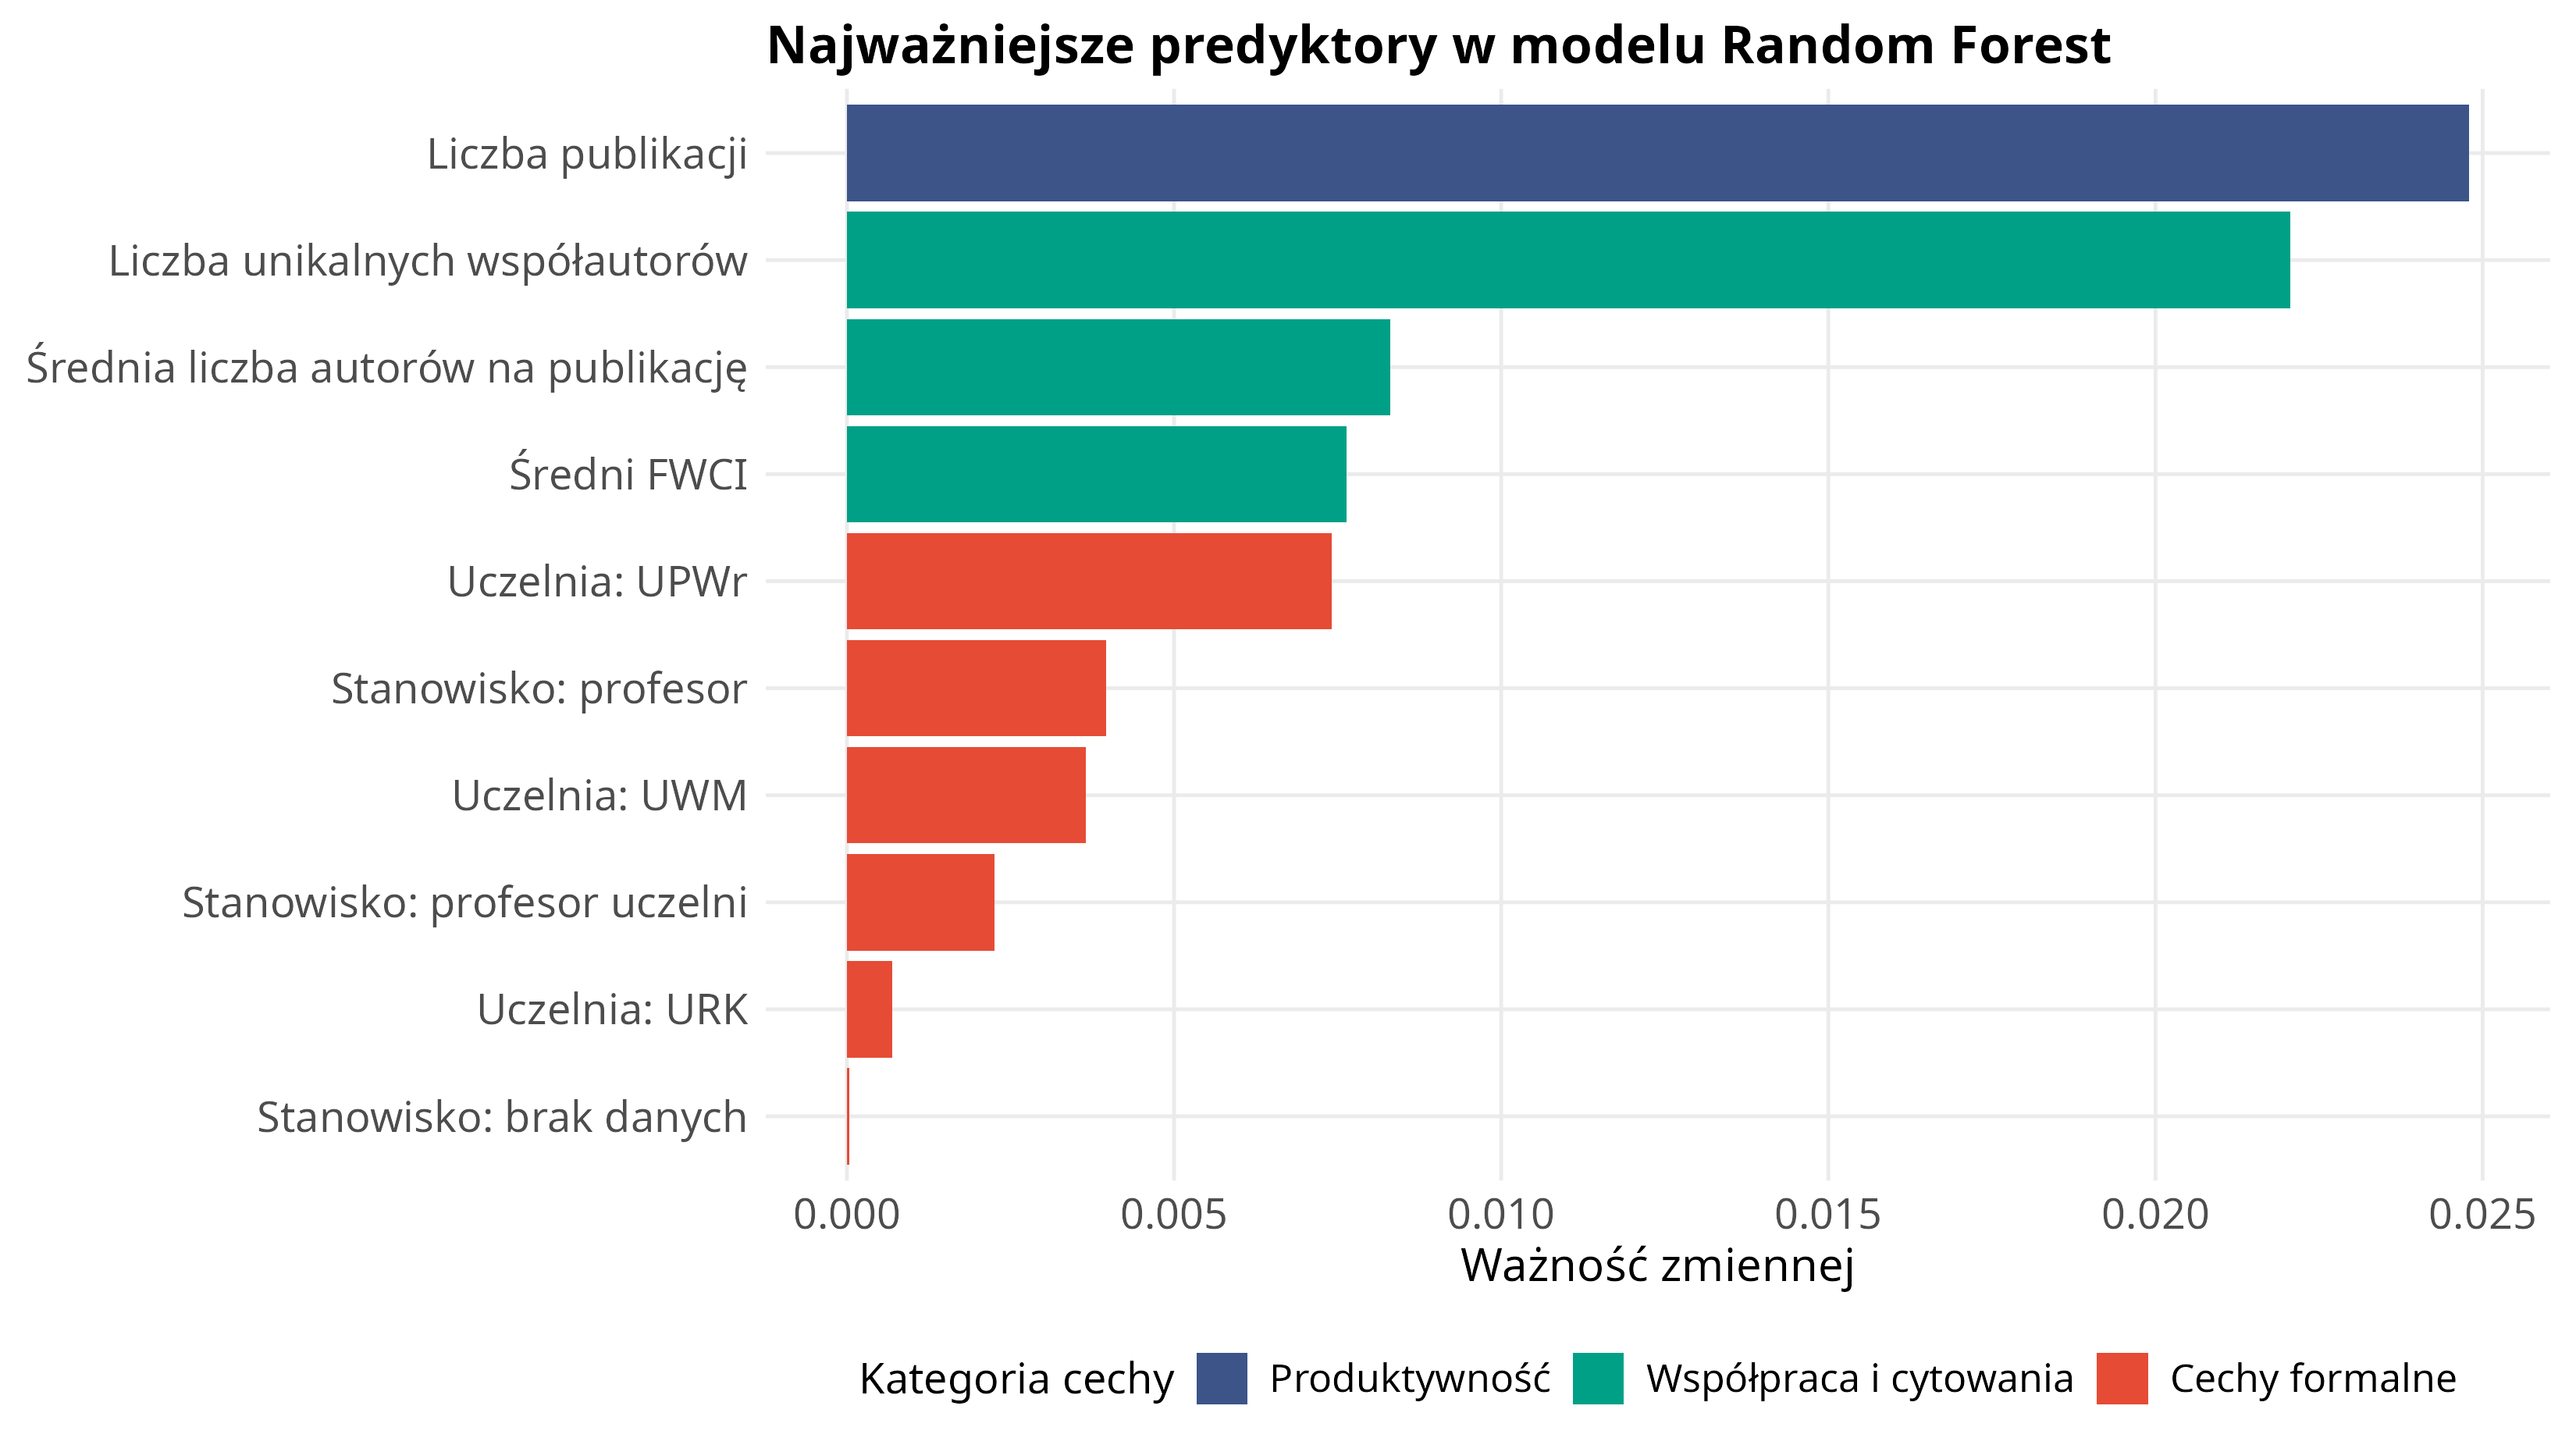
\includegraphics[width=1\linewidth,height=\textheight,keepaspectratio]{../Wykresy/praca/fig_04b_waznosc.png}

}

\caption{\label{fig-waznosc}Najważniejsze predyktory wysokiego wpływu
publikacyjnego w modelu Random Forest (ważność permutacyjna). Kolor
oznacza kategorię cechy: produktywność, współpraca i cytowania oraz
cechy formalne (uczelnia, stanowisko).}

\end{figure}%

W odpowiedzi na pytanie 3 wyniki pokazują, że wysoki wpływ naukowy można
przewidywać na podstawie cech badacza, takich jak stanowisko, uczelnia,
liczba publikacji i współpraca naukowa. Model osiągnął bardzo dobrą
zdolność rozróżniania osób o wysokim i niższym wpływie naukowym (AUC ok.
0,97).

\subsubsection{Model jakościowy: czy wysoki wpływ publikacyjny zależy
tylko od
stażu?}\label{model-jakoux15bciowy-czy-wysoki-wpux142yw-publikacyjny-zaleux17cy-tylko-od-staux17cu}

Poprzedni model przewidywał sumaryczny IF, czyli wskaźnik kumulatywny.
Taki wskaźnik rośnie wraz z liczbą publikacji, dlatego duże znaczenie
liczby publikacji w modelu było oczekiwane. Z tego powodu zbudowano
drugi model, który miał sprawdzić nie wielkość dorobku, lecz jego
jakość.

W tym modelu zmienną celu była wysoka jakość publikacji, określona jako
średni FWCI większy niż 1. Oznacza to, że publikacje danej osoby były
cytowane powyżej średniej światowej w swojej dziedzinie. Do tej grupy
należały 234 z 366 osób z dostępnymi danymi OpenAlex, czyli 63,9 \%. Z
modelu usunięto zmienne bezpośrednio związane z IF, a dodano wiek
akademicki, czyli liczbę lat od pierwszej publikacji.

Wyniki są istotne z dwóch powodów. Po pierwsze, jakość dorobku jest
trudniejsza do przewidywania niż jego skumulowana wielkość. AUC modelu
jakościowego wyniosło około 0,81 (RF 0,807; XGBoost 0,810), podczas gdy
w modelu ilościowym było bliskie 0,97.

Po drugie, w modelu jakościowym największego znaczenia nie miały ani
wiek akademicki, ani liczba publikacji. Najważniejsze okazały się cechy
związane ze współpracą naukową, przede wszystkim średnia liczba autorów
jednej publikacji oraz liczba unikalnych współautorów. Stanowisko i
uczelnia miały niewielkie znaczenie (Rysunek~\ref{fig-waznosc-jakosc}).

\begin{figure}[H]

\centering{

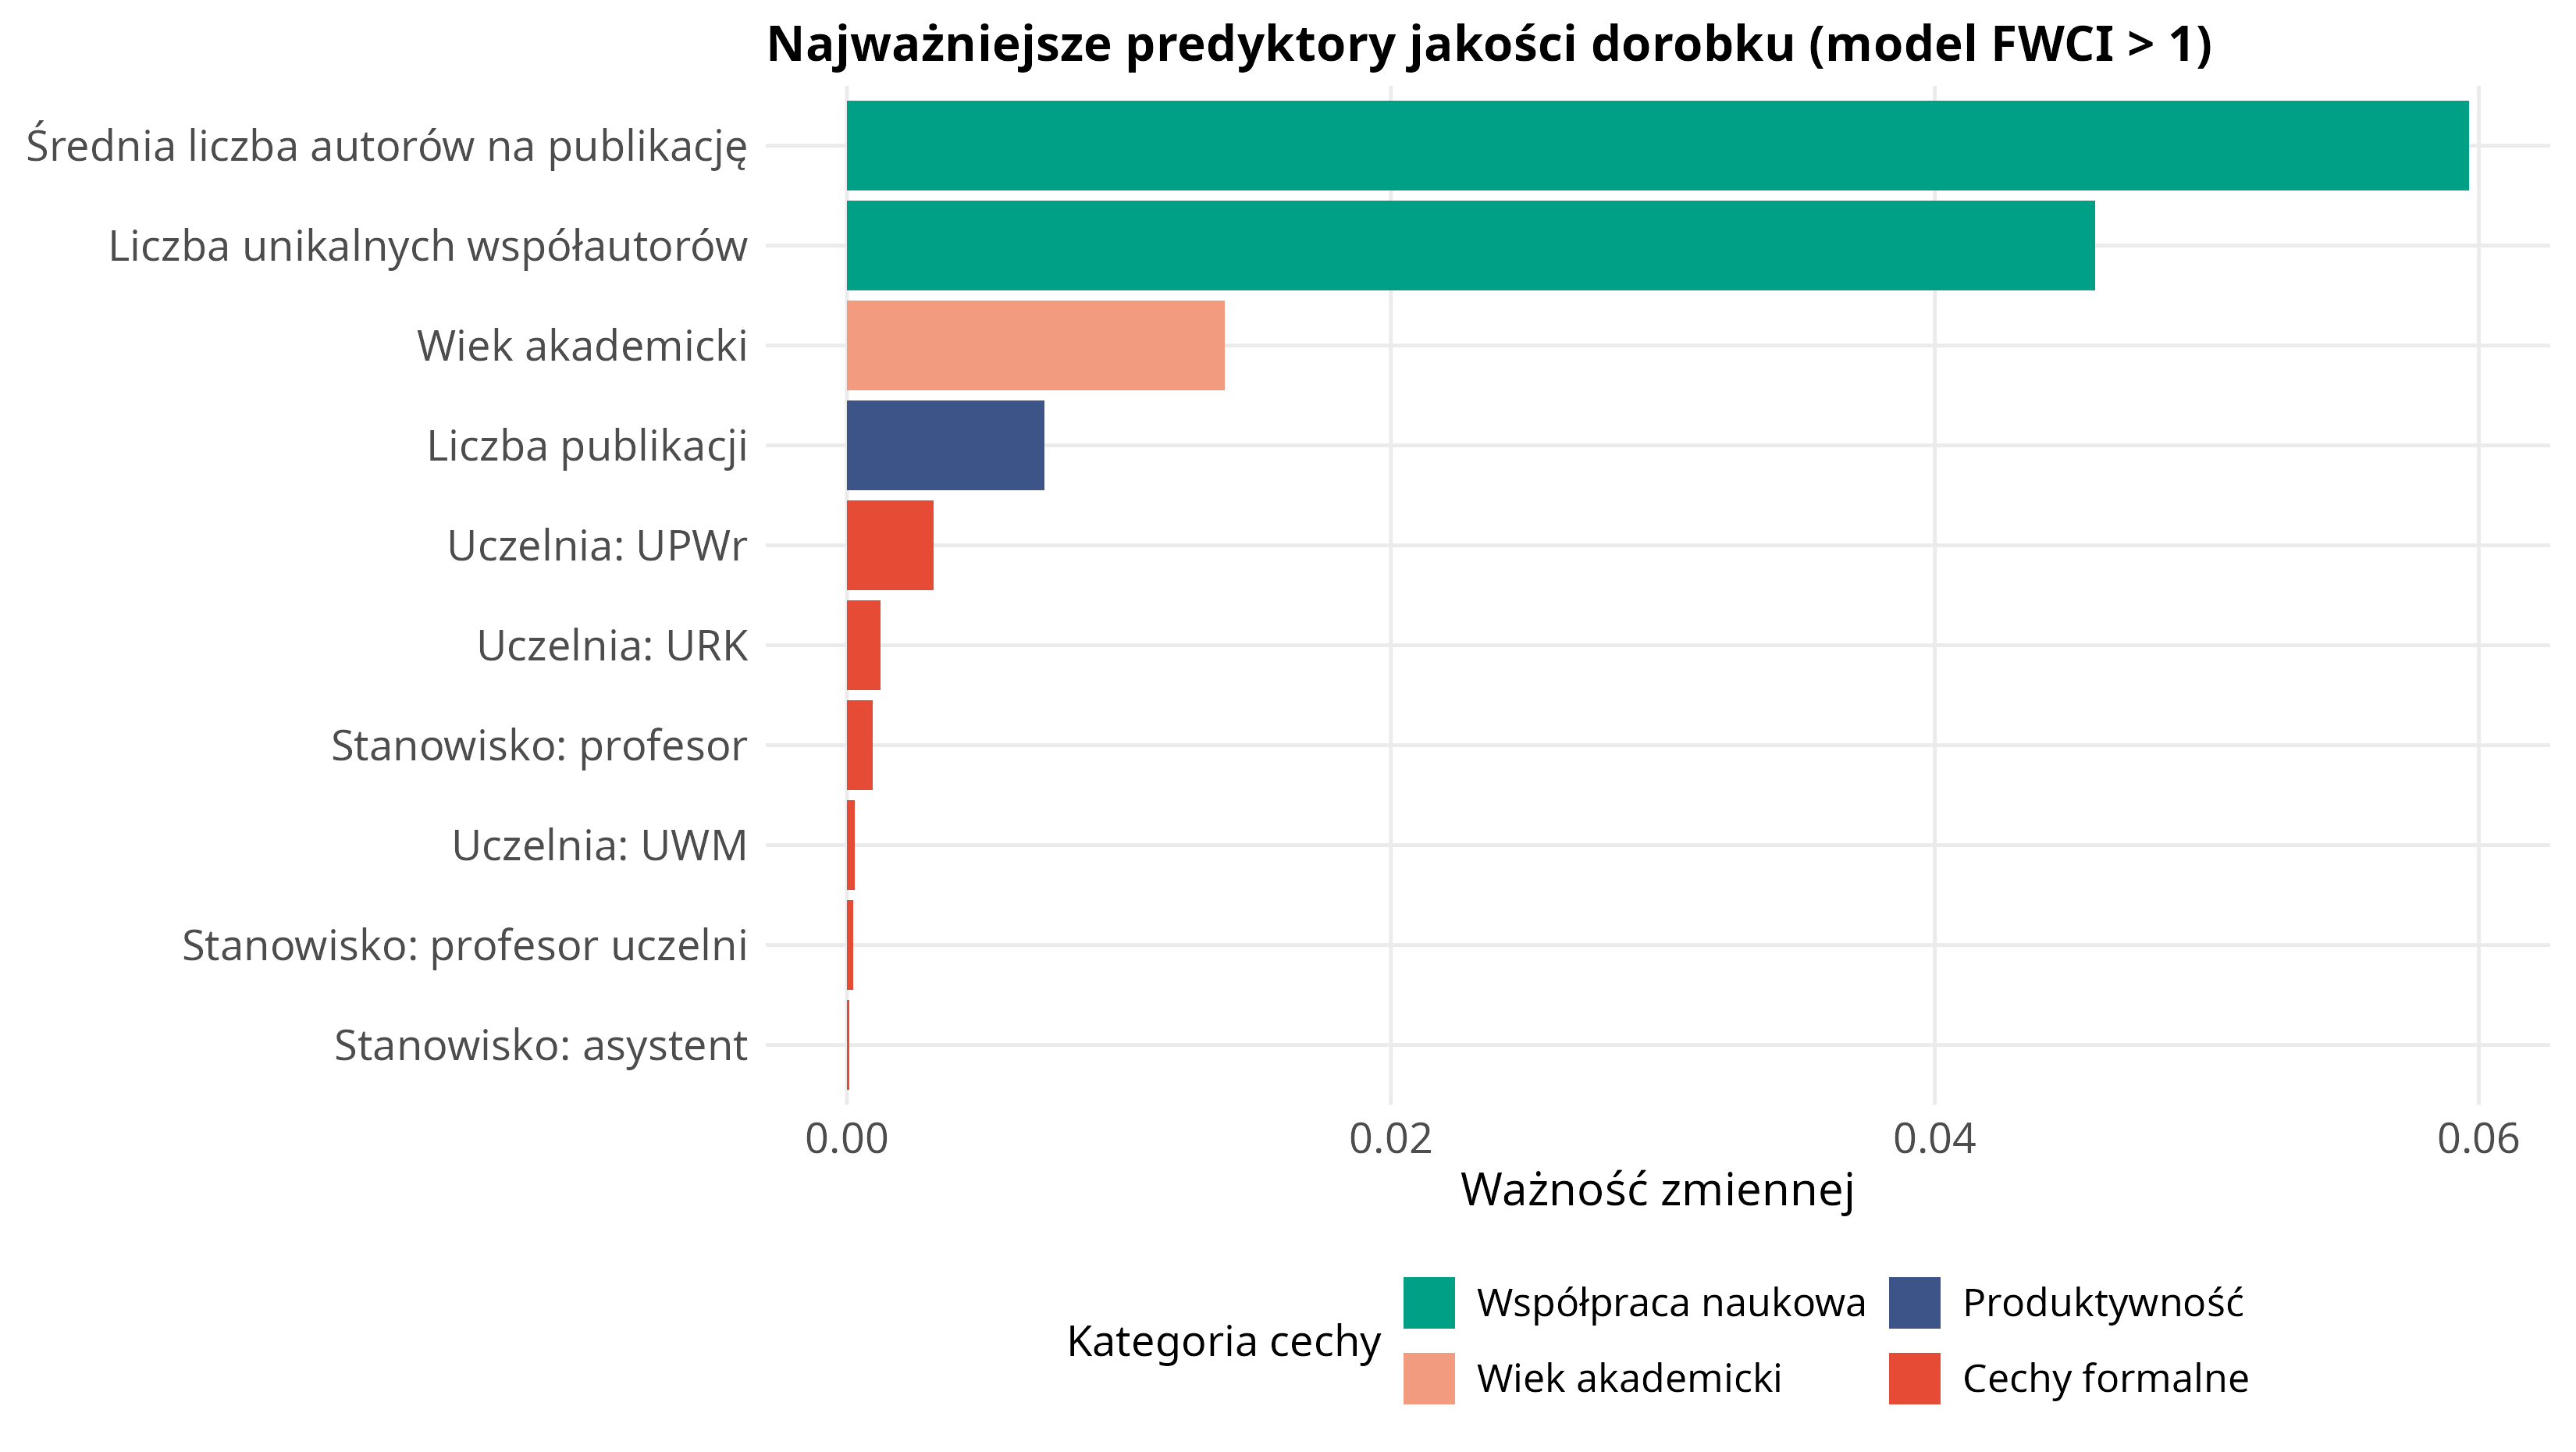
\includegraphics[width=1\linewidth,height=\textheight,keepaspectratio]{../Wykresy/praca/fig_04c_waznosc_jakosc.png}

}

\caption{\label{fig-waznosc-jakosc}Najważniejsze predyktory jakości
dorobku w modelu Random Forest. Model przewidywał, czy średni FWCI
badacza przekracza 1. Największe znaczenie miały cechy współpracy
naukowej, zwłaszcza średnia liczba autorów jednej publikacji i liczba
unikalnych współautorów. Wiek akademicki, liczba publikacji, stanowisko
i uczelnia miały mniejsze znaczenie. Kolor oznacza kategorię zmiennej.}

\end{figure}%

Oznacza to, że wysoki wpływ pojedynczych publikacji częściej wiąże się z
pracą w szerszych, wieloautorskich zespołach niż ze stażem, liczbą
publikacji czy formalnym stanowiskiem. Podobny wniosek wynikał już z
analizy klastrów, w której wyróżniono profil jakościowy obejmujący wielu
młodszych badaczy. Pokazuje to, że wysoka jakość dorobku nie musi być
związana z długim stażem ani dużą liczbą publikacji.

\subsection{Sieć współautorstwa (pytanie
4)}\label{sieux107-wspuxf3ux142autorstwa-pytanie-4}

Sieć współautorstwa utworzono na podstawie danych OpenAlex. Uwzględniono
tylko współprace między osobami z badanej próby oraz tylko takie pary
autorów, które miały co najmniej dwie wspólne publikacje. Ostateczna
sieć obejmowała 367 badaczy i 630 połączeń między nimi.

Największa spójna część sieci, czyli grupa badaczy połączonych ze sobą
bezpośrednio lub pośrednio przez współautorów, liczyła 265 osób.
Stanowiło to 72 \% wszystkich węzłów sieci. W tej części znajdowało się
595 połączeń. Gęstość sieci wyniosła 0,017, a współczynnik gronowania
0,37.

\begin{figure}[H]

\centering{

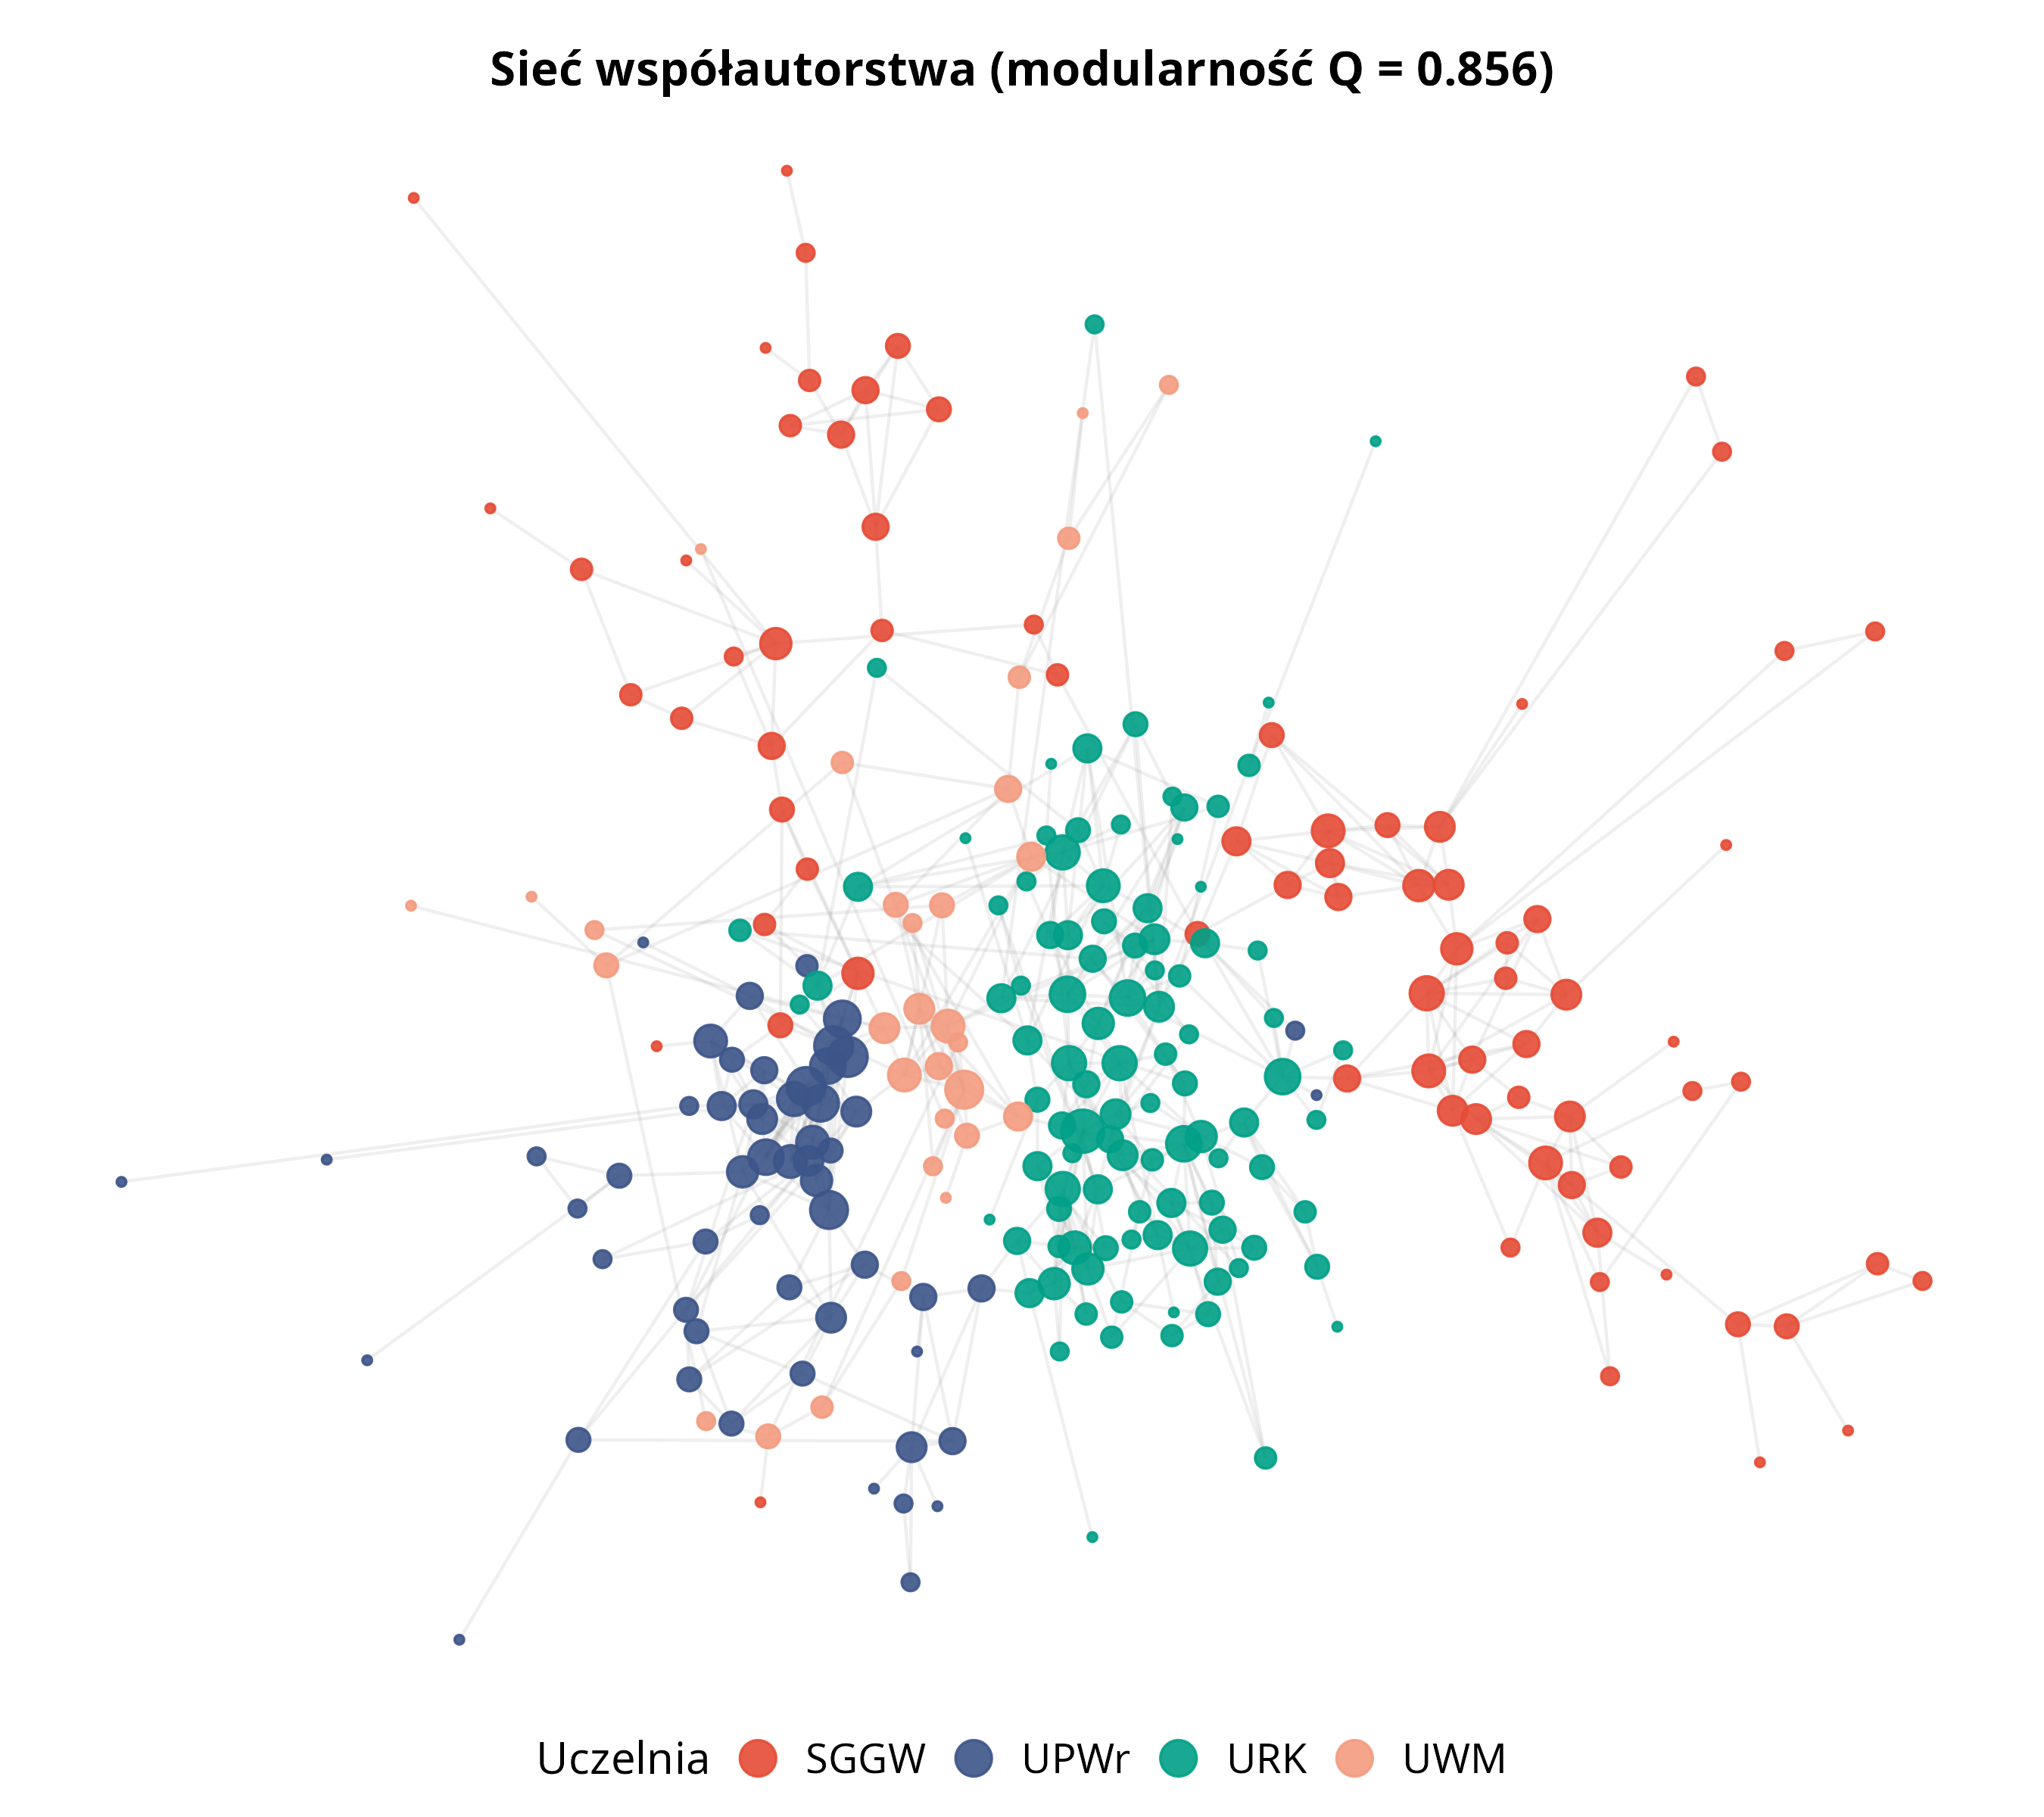
\includegraphics[width=0.95\linewidth,height=\textheight,keepaspectratio]{../Wykresy/praca/fig_05a_siec.png}

}

\caption{\label{fig-siec}Sieć współautorstwa naukowców badanej
dyscypliny. Węzły to badacze (kolor oznacza uczelnię, wielkość liczbę
połączeń), a krawędzie wspólne publikacje. Skupiska tej samej barwy
pokazują, że współpraca koncentruje się wewnątrz uczelni.}

\end{figure}%

Wykrywanie wspólnot metodą Louvain pozwoliło wyodrębnić 21 społeczności
współautorskich. Metoda ta wyszukuje w sieci grupy silniej połączone
wewnętrznie niż z resztą sieci, czyli zespoły badaczy, którzy częściej
publikują między sobą niż z osobami spoza grupy. Wysoka modularność (Q =
0,856) wskazuje na wyraźny podział sieci na odrębne środowiska
współpracy (Rysunek~\ref{fig-siec}). Modularność przyjmuje wartości od 0
do około 1: im wyższa, tym silniej sieć dzieli się na grupy gęsto
połączone wewnątrz i słabo między sobą. Wartości powyżej 0,3--0,4 uznaje
się już za wyraźną strukturę społecznościową, więc poziom 0,856 jest
bardzo wysoki.

Następnie sprawdzono, czy te społeczności pokrywają się raczej z
podziałem na uczelnie, czy na stanowiska. Porównano w tym celu podział
sieci na społeczności z podziałem według uczelni oraz według stanowiska,
używając skorygowanego indeksu Randa (ARI)
(\citeproc{ref-hubert1985}{Hubert i Arabie 1985}) i znormalizowanej
informacji wzajemnej (NMI). Obie miary mówią, jak bardzo dwa podziały są
do siebie podobne. Przyjmują wartość 1, gdy podziały są identyczne, i
wartości bliskie 0, gdy są zasadniczo niezależne (dla ARI poziom 0
odpowiada zgodności na poziomie losowym, a nie brakowi wspólnych
elementów); im wyższa wartość, tym większa zgodność
(Tabela~\ref{tbl-spolecznosci}).

\global\setlength{\Oldarrayrulewidth}{\arrayrulewidth}

\global\setlength{\Oldtabcolsep}{\tabcolsep}

\setlength{\tabcolsep}{2pt}

\renewcommand*{\arraystretch}{1.5}



\providecommand{\ascline}[3]{\noalign{\global\arrayrulewidth #1}\arrayrulecolor[HTML]{#2}\cline{#3}}

\begin{longtable}[c]{|p{3.30in}|p{1.25in}|p{1.25in}}

\caption{\label{tbl-spolecznosci}Zgodność społeczności Louvain ze
zmiennymi opisowymi (ARI, NMI).}

\tabularnewline

\ascline{1.5pt}{666666}{1-3}

\multicolumn{1}{>{\centering}m{\dimexpr 3.3in+0\tabcolsep}}{\textcolor[HTML]{000000}{\fontsize{10}{10}\selectfont{\global\setmainfont{Latin Modern Roman}{Porównanie}}}} & \multicolumn{1}{>{\centering}m{\dimexpr 1.25in+0\tabcolsep}}{\textcolor[HTML]{000000}{\fontsize{10}{10}\selectfont{\global\setmainfont{Latin Modern Roman}{ARI}}}} & \multicolumn{1}{>{\centering}m{\dimexpr 1.25in+0\tabcolsep}}{\textcolor[HTML]{000000}{\fontsize{10}{10}\selectfont{\global\setmainfont{Latin Modern Roman}{NMI}}}} \\

\ascline{1.5pt}{666666}{1-3}\endfirsthead 

\ascline{1.5pt}{666666}{1-3}

\multicolumn{1}{>{\centering}m{\dimexpr 3.3in+0\tabcolsep}}{\textcolor[HTML]{000000}{\fontsize{10}{10}\selectfont{\global\setmainfont{Latin Modern Roman}{Porównanie}}}} & \multicolumn{1}{>{\centering}m{\dimexpr 1.25in+0\tabcolsep}}{\textcolor[HTML]{000000}{\fontsize{10}{10}\selectfont{\global\setmainfont{Latin Modern Roman}{ARI}}}} & \multicolumn{1}{>{\centering}m{\dimexpr 1.25in+0\tabcolsep}}{\textcolor[HTML]{000000}{\fontsize{10}{10}\selectfont{\global\setmainfont{Latin Modern Roman}{NMI}}}} \\

\ascline{1.5pt}{666666}{1-3}\endhead



\multicolumn{1}{>{\raggedright}m{\dimexpr 3.3in+0\tabcolsep}}{\textcolor[HTML]{000000}{\fontsize{10}{10}\selectfont{\global\setmainfont{Latin Modern Roman}{Społeczność\ vs\ uczelnia}}}} & \multicolumn{1}{>{\centering}m{\dimexpr 1.25in+0\tabcolsep}}{\textcolor[HTML]{000000}{\fontsize{10}{10}\selectfont{\global\setmainfont{Latin Modern Roman}{0,233}}}} & \multicolumn{1}{>{\centering}m{\dimexpr 1.25in+0\tabcolsep}}{\textcolor[HTML]{000000}{\fontsize{10}{10}\selectfont{\global\setmainfont{Latin Modern Roman}{0,575}}}} \\





\multicolumn{1}{>{\raggedright}m{\dimexpr 3.3in+0\tabcolsep}}{\textcolor[HTML]{000000}{\fontsize{10}{10}\selectfont{\global\setmainfont{Latin Modern Roman}{Społeczność\ vs\ stanowisko}}}} & \multicolumn{1}{>{\centering}m{\dimexpr 1.25in+0\tabcolsep}}{\textcolor[HTML]{000000}{\fontsize{10}{10}\selectfont{\global\setmainfont{Latin Modern Roman}{0,009}}}} & \multicolumn{1}{>{\centering}m{\dimexpr 1.25in+0\tabcolsep}}{\textcolor[HTML]{000000}{\fontsize{10}{10}\selectfont{\global\setmainfont{Latin Modern Roman}{0,092}}}} \\

\ascline{1.5pt}{666666}{1-3}



\multicolumn{3}{>{\raggedright}m{\dimexpr 5.8in+4\tabcolsep}}{\textcolor[HTML]{000000}{\fontsize{9}{9}\selectfont{\global\setmainfont{Latin Modern Roman}{ARI\ (skorygowany\ indeks\ Randa)\ i\ NMI\ (znormalizowana\ informacja\ wzajemna)\ mierzą\ zgodność\ dwóch\ podziałów.}}}} \\





\multicolumn{3}{>{\raggedright}m{\dimexpr 5.8in+4\tabcolsep}}{\textcolor[HTML]{000000}{\fontsize{9}{9}\selectfont{\global\setmainfont{Latin Modern Roman}{Wartość\ 1\ oznacza\ podziały\ identyczne,\ a\ wartości\ bliskie\ 0\ podziały\ niezależne\ (dla\ ARI\ poziom\ 0\ odpowiada\ zgodności\ losowej,\ a\ nie\ brakowi\ wspólnych\ elementów).}}}} \\




\end{longtable}

\arrayrulecolor[HTML]{000000}

\global\setlength{\arrayrulewidth}{\Oldarrayrulewidth}

\global\setlength{\tabcolsep}{\Oldtabcolsep}

\renewcommand*{\arraystretch}{1}

\begin{figure}[H]

\centering{

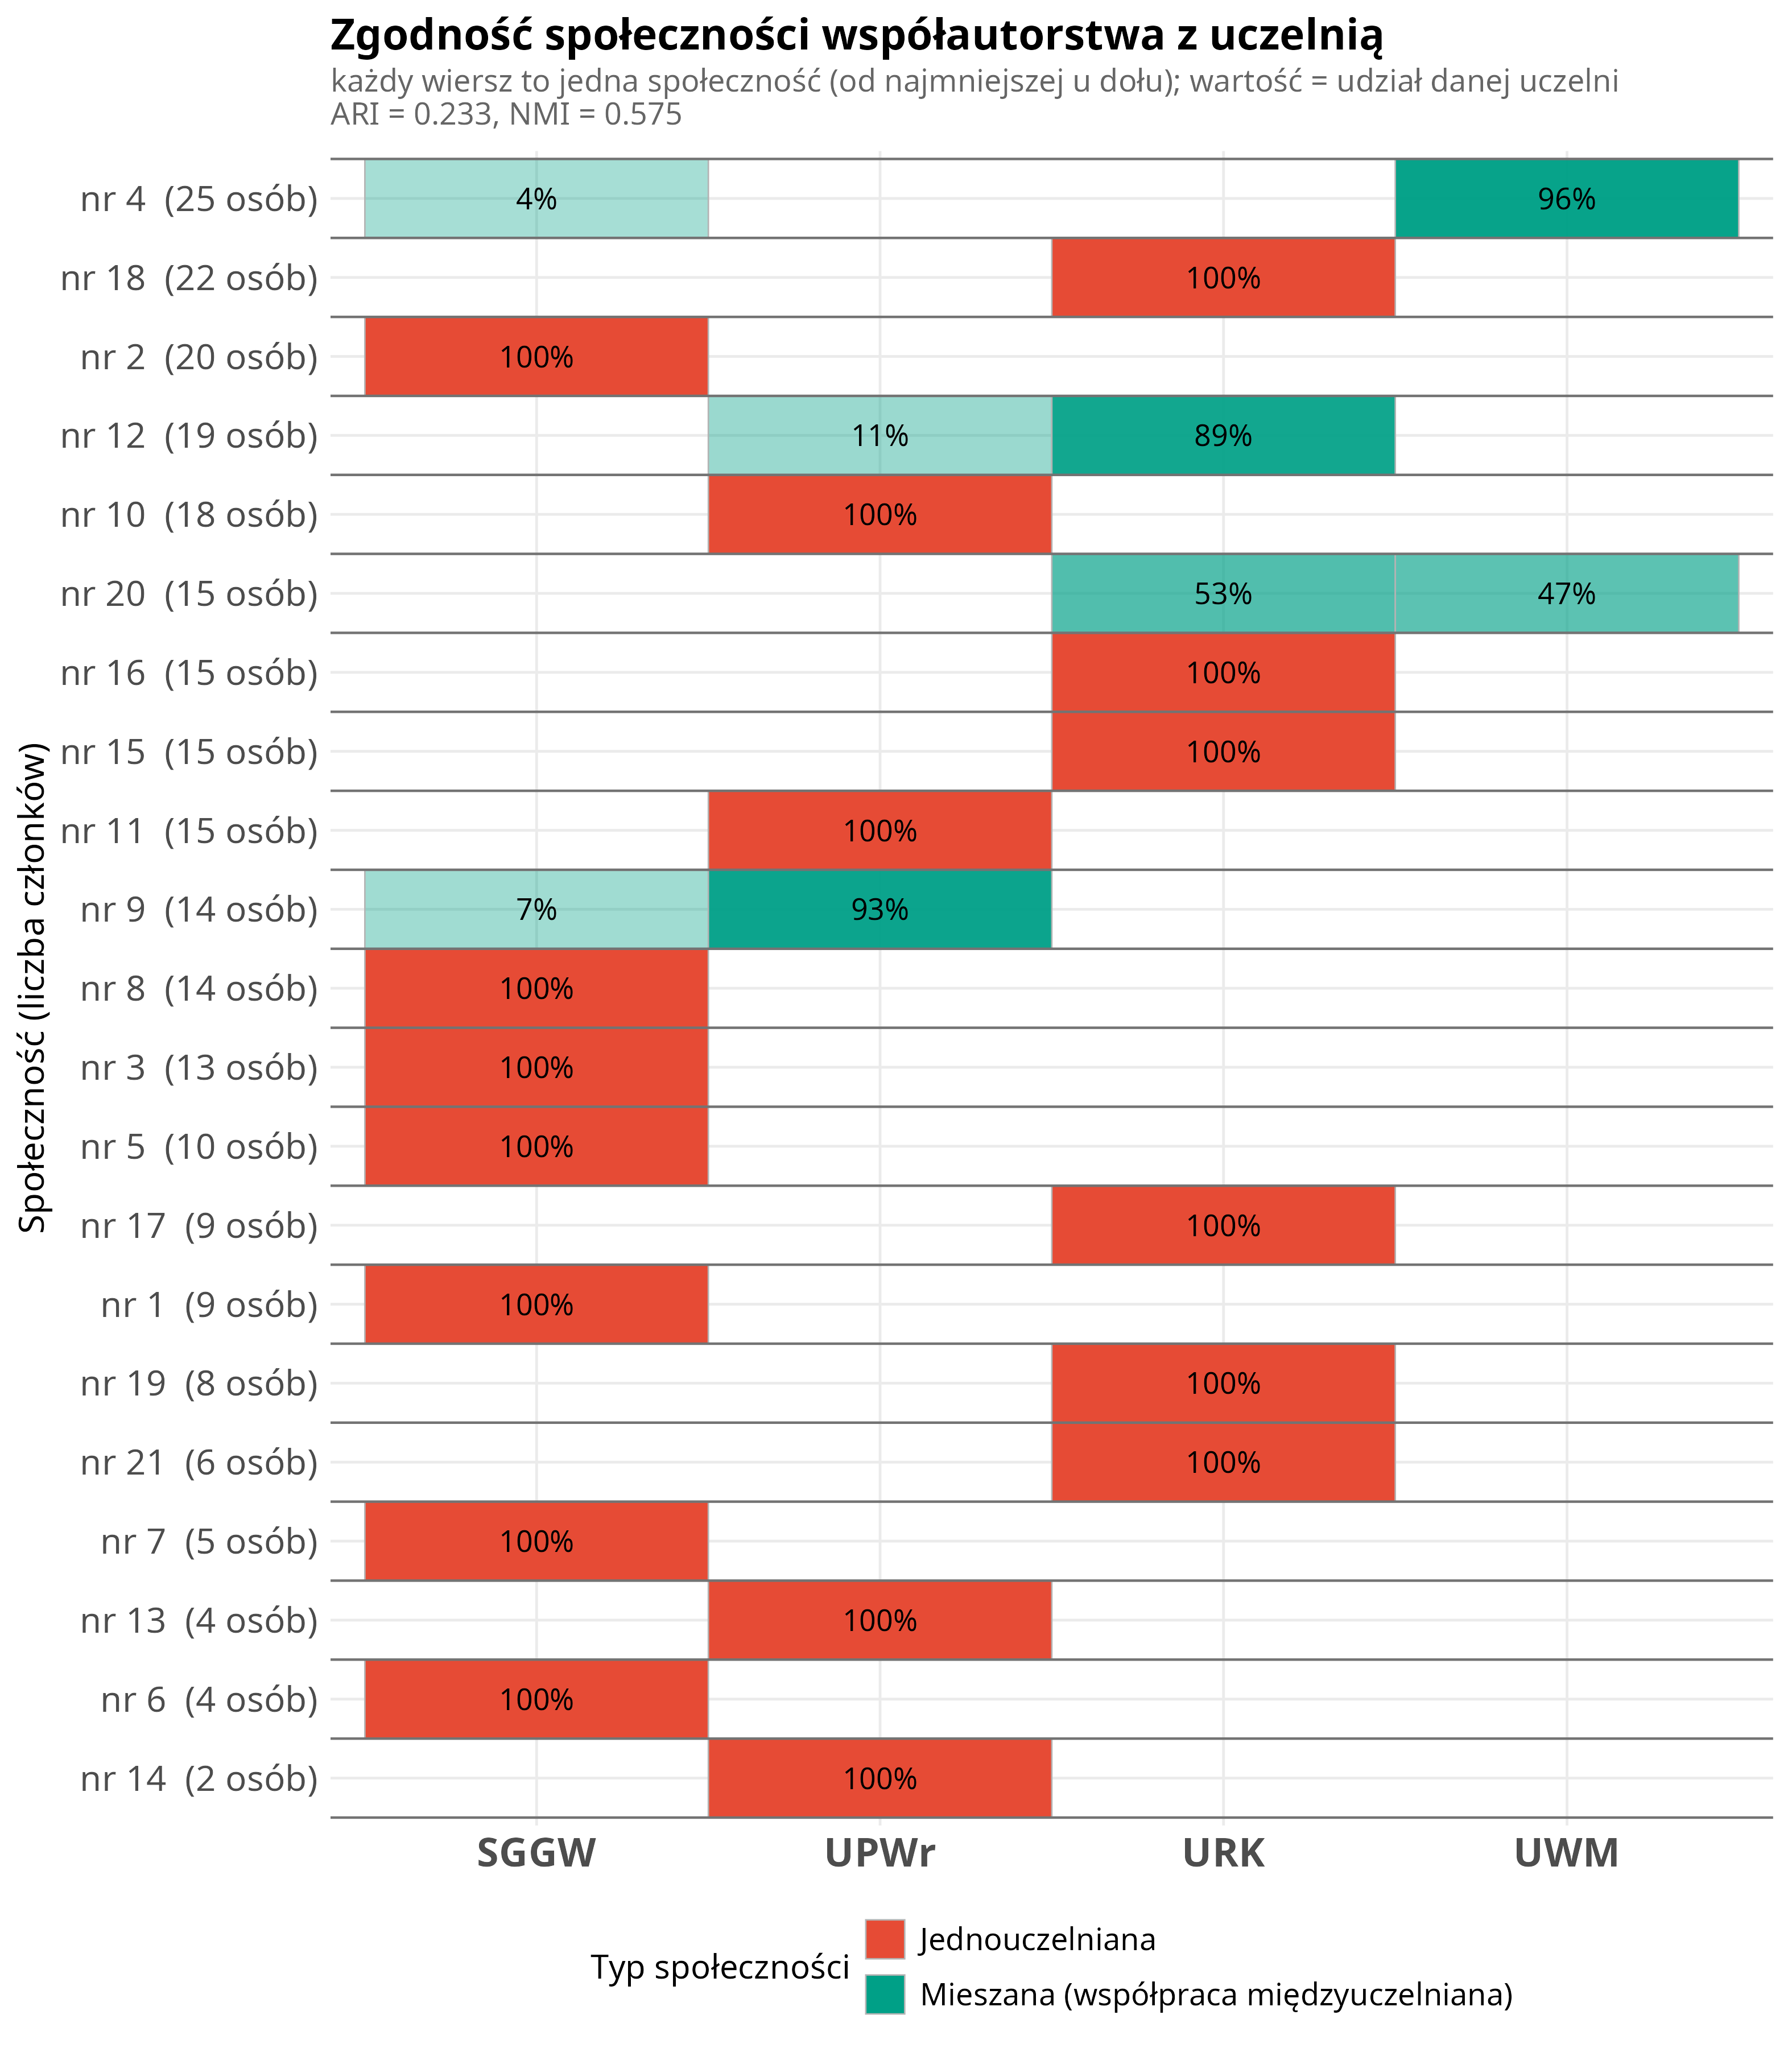
\includegraphics[width=1\linewidth,height=\textheight,keepaspectratio]{../Wykresy/praca/fig_05b_spolecznosci.png}

}

\caption{\label{fig-spolecznosci}Zgodność społeczności Louvain z
uczelnią. Każdy wiersz to jedna społeczność (uporządkowane według
wielkości); wartość i intensywność oznaczają udział danej uczelni, a
kolor typ społeczności: czerwień to społeczność jednouczelniana, turkus
to społeczność mieszana (współpraca międzyuczelniana). Niemal wszystkie
społeczności są jednorodne uczelniano.}

\end{figure}%

Społeczności współautorskie są znacznie silniej związane z uczelnią niż
ze stanowiskiem. Zgodność społeczności z uczelnią jest wyraźna (NMI =
0,58), natomiast zgodność ze stanowiskiem jest bardzo słaba (NMI =
0,09). Oznacza to, że autorzy łączą się w grupy współpracy głównie
według afiliacji uczelnianej, a nie według pozycji akademickiej.

Potwierdza to heatmapa zgodności (Rysunek~\ref{fig-spolecznosci}).
Większość społeczności składa się w całości lub prawie w całości z osób
z jednej uczelni. Społeczności międzyuczelniane występują, ale są
nieliczne. Współpraca naukowa w badanej dyscyplinie ma więc przede
wszystkim charakter wewnątrzinstytucjonalny.

Najwyższą centralność stopnia, czyli największą liczbę bezpośrednich
powiązań współautorskich, osiąga profesor z URK (S. Smoleń). Wśród
najbardziej centralnych osób znajduje się także grupa badaczy
gleboznawczych z UPWr.

\section{Dyskusja}\label{dyskusja}

\subsection{Dwoistość: profil indywidualny a struktura
współpracy}\label{dwoistoux15bux107-profil-indywidualny-a-struktura-wspuxf3ux142pracy}

Analiza danych wykazuje, że indywidualny dorobek naukowców i ich
współpraca naukowa układają się według różnych zasad. Dorobek
pojedynczych badaczy jest związany przede wszystkim ze stanowiskiem,
czyli pośrednio ze stażem i etapem kariery. Pokazały to zarówno
porównania wskaźników bibliometrycznych, jak i analiza klastrów.
Wskaźniki dorobku rosną zwykle od adiunktów, przez profesorów uczelni,
do profesorów. Również przynależność do klastra o wysokim dorobku jest
silnie związana ze stanowiskiem (Craméra V = 0,45), a tylko słabo z
uczelnią (V = 0,10).

Warto odnotować bardzo wysoką korelację sumarycznego IF z punktacją MEiN
(r = 0,95, w trzech uczelniach udostępniających tę metrykę). Na poziomie
zagregowanym polski system punktacji czasopism, mimo powszechnej krytyki
jego stabilności, w analizowanej dyscyplinie silnie odzwierciedla
międzynarodowy Impact Factor. Spójnie z tym wskaźnik IF / MEiN nie
różnicował istotnie badanych grup (p = 0,075), co sugeruje, że relacja
punktów do IF jest zbliżona niezależnie od uczelni i stanowiska, choć
przy granicznej istotności wniosek ten wymaga ostrożności.

Inaczej wygląda sieć współautorstwa. Wspólnoty wykryte w sieci pokrywają
się przede wszystkim z uczelnią, a nie ze stanowiskiem. Zgodność
społeczności z uczelnią jest wyraźna (NMI = 0,58), natomiast zgodność ze
stanowiskiem jest bardzo słaba (NMI = 0,09). Oznacza to, że badacze o
podobnym poziomie dorobku mogą pracować w różnych uczelniach, ale
faktyczna współpraca naukowa najczęściej przebiega wewnątrz instytucji.

Innymi słowy, profil bibliometryczny naukowca zależy głównie od etapu
kariery, a nie od macierzystej uczelni. Natomiast struktura współpracy
naukowej jest związana przede wszystkim z afiliacją. Badacze najczęściej
współpracują z osobami z tej samej instytucji, a współprace
międzyuczelniane są stosunkowo nieliczne. Potwierdza to wysoka
modularność sieci (Q = 0,856), wskazująca na wyraźnie oddzielone grupy
współautorskie.

Taki układ może wynikać ze specyfiki nauk rolniczych. W tej dziedzinie
część badań jest silnie związana z lokalną infrastrukturą i warunkami
prowadzenia eksperymentów, takimi jak pola doświadczalne, stacje
badawcze czy lokalne uwarunkowania glebowo-klimatyczne. Może to sprzyjać
współpracy w obrębie tej samej uczelni lub ośrodka badawczego.

\subsection{Predyktory wysokiego wpływu
publikacyjnego}\label{predyktory-wysokiego-wpux142ywu-publikacyjnego}

Modelowanie predykcyjne pokazuje, że wysoki wpływ publikacyjny,
zdefiniowany jako przynależność do górnego decyla sumarycznego IF, można
dobrze przewidywać na podstawie cech badacza. Model osiągnął bardzo
dobrą zdolność rozróżniania osób o wysokim i niższym wpływie
publikacyjnym (AUC ok. 0,97). Najważniejsze znaczenie miały liczba
publikacji oraz cechy współpracy naukowej, zwłaszcza liczba unikalnych
współautorów i średni FWCI. Znacznie mniejsze znaczenie miały natomiast
stanowisko i uczelnia.

Wynik ten sugeruje, że wysoki skumulowany wpływ publikacyjny wiąże się
przede wszystkim z produktywnością oraz udziałem w sieci współpracy, a
nie bezpośrednio z formalną pozycją akademicką czy afiliacją. Niska
czułość modelu przy domyślnym progu klasyfikacji 0,5 wynikała głównie z
niedopasowania progu do rzadkiej klasy wysokiego wpływu, a nie ze słabej
jakości modelu. Po obniżeniu progu na podstawie danych walidacyjnych
model poprawnie identyfikował wszystkie osoby z grupy wysokiego wpływu
publikacyjnego (czułość = 1,00), przy zbalansowanej trafności 0,87.

Model jakościowy uzupełnia tę interpretację. Gdy zmienną celu była
jakość dorobku, zdefiniowana jako średni FWCI większy niż 1, wyniki były
słabsze niż w modelu ilościowym (AUC ok. 0,81). Zmieniła się także
hierarchia predyktorów. Liczba publikacji i wiek akademicki miały
mniejsze znaczenie, natomiast na pierwszy plan wysunęły się cechy
współpracy naukowej, zwłaszcza średnia liczba autorów jednej publikacji
oraz liczba unikalnych współautorów.

Oznacza to, że skumulowany wpływ publikacyjny jest silnie związany z
wielkością dorobku, ale jakość pojedynczych publikacji zależy bardziej
od sposobu współpracy naukowej niż od stażu czy formalnego stanowiska.
Wynik ten pokazuje, że wysoki wpływ publikacyjny nie jest wyłącznie
efektem długiego stażu akademickiego. Podobny wniosek wynikał już z
analizy klastrów, w której wyróżniono profil jakościowy obejmujący wielu
młodszych badaczy.

Spójny obraz daje też wariant klastrowania k = 3, w którym wyodrębniono
profil jakościowy zdominowany przez asystentów i adiunktów o wysokim
FWCI i IF na publikację. Może to odzwierciedlać zmianę pokoleniową, w
której młodsi badacze częściej publikują w prestiżowych czasopismach o
szerokim zasięgu, w ramach większych zespołów współautorskich, zamiast
budować dużą liczbę prac o niższym oddziaływaniu. Ponieważ dane mają
charakter przekrojowy, interpretację tę należy traktować jako hipotezę:
nie można odróżnić rzeczywistego efektu pokoleniowego od efektu etapu
kariery ani od selekcji osób pozostających w nauce.

\subsection{Kategoria ewaluacyjna
MEiN}\label{kategoria-ewaluacyjna-mein}

Kategorii ewaluacyjnej MEiN nie można było analizować jako niezależnego
czynnika, ponieważ w badanej próbie była ona ściśle powiązana z
uczelnią. Tylko UWM miała kategorię B+, natomiast pozostałe trzy
uczelnie miały kategorię A. Nie da się więc rozstrzygnąć, czy ewentualne
różnice wynikają z kategorii ewaluacyjnej, czy ze specyfiki konkretnej
uczelni.

Na poziomie opisowym UWM nie wypada jednak wyraźnie słabiej niż uczelnie
kategorii A. Mediany jej wskaźników bibliometrycznych mieszczą się w
zakresie wartości obserwowanych w pozostałych uczelniach. Sugeruje to,
że formalna kategoria ewaluacyjna nie musi bezpośrednio przekładać się
na indywidualne wskaźniki bibliometryczne badanych pracowników.

Wniosek ten należy jednak traktować ostrożnie. W badaniu uwzględniono
tylko jedną uczelnię z kategorią B+, dlatego zależność między kategorią
ewaluacyjną a indywidualnym dorobkiem naukowców wymagałaby sprawdzenia
na większej próbie uczelni.

\subsection{Dynamika rozwoju a wrażliwość na źródło
danych}\label{dynamika-rozwoju-a-wraux17cliwoux15bux107-na-ux17aruxf3dux142o-danych}

Statyczną analizę dorobku uzupełniono analizą tempa rozwoju
produktywności publikacyjnej poszczególnych uczelni. Tempo to mierzono
jako roczny wzrost liczby publikacji na badacza w latach 2008--2024.
Analizę wykonano dwukrotnie: najpierw na podstawie danych OpenAlex, a
następnie na podstawie pełnych list publikacji z systemu Omega-PSIR.

Wyniki okazały się silnie zależne od źródła danych. W danych OpenAlex
wszystkie uczelnie miały bardzo podobne tempo wzrostu, mieszczące się w
wąskim zakresie od 4,0 \% do 4,6 \% rocznie. Najwyższą wartość uzyskała
SGGW (4,6 \%), następnie URK (4,2 \%), UPWr (4,1 \%) i UWM (4,0 \%). Na
podstawie OpenAlex trudno więc wskazać wyraźne różnice między
uczelniami.

Inny obraz uzyskano po powtórzeniu analizy na pełnych listach publikacji
Omega-PSIR, obejmujących 491 osób i także te publikacje, które nie są
indeksowane w OpenAlex, np. część polskich czasopism i monografii. W tym
ujęciu najwyższe tempo wzrostu miały URK (5,4 \%) i UWM (4,9 \%),
natomiast niższe UPWr (2,7 \%) i SGGW (1,2 \%)
(Rysunek~\ref{fig-dynamika}). Najbardziej widoczna różnica dotyczy SGGW:
w danych OpenAlex uczelnia ta miała najwyższe tempo wzrostu, natomiast w
danych Omega-PSIR znalazła się na ostatnim miejscu.

Wynik ten utrzymał się także po ograniczeniu analizy do osób o dłuższym
stażu publikacyjnym, czyli takich, których pierwsza publikacja ukazała
się nie później niż w 2010 r. Oznacza to, że obserwowane różnice nie
wynikają wyłącznie z napływu młodszych badaczy do próby.

\begin{figure}[H]

\centering{

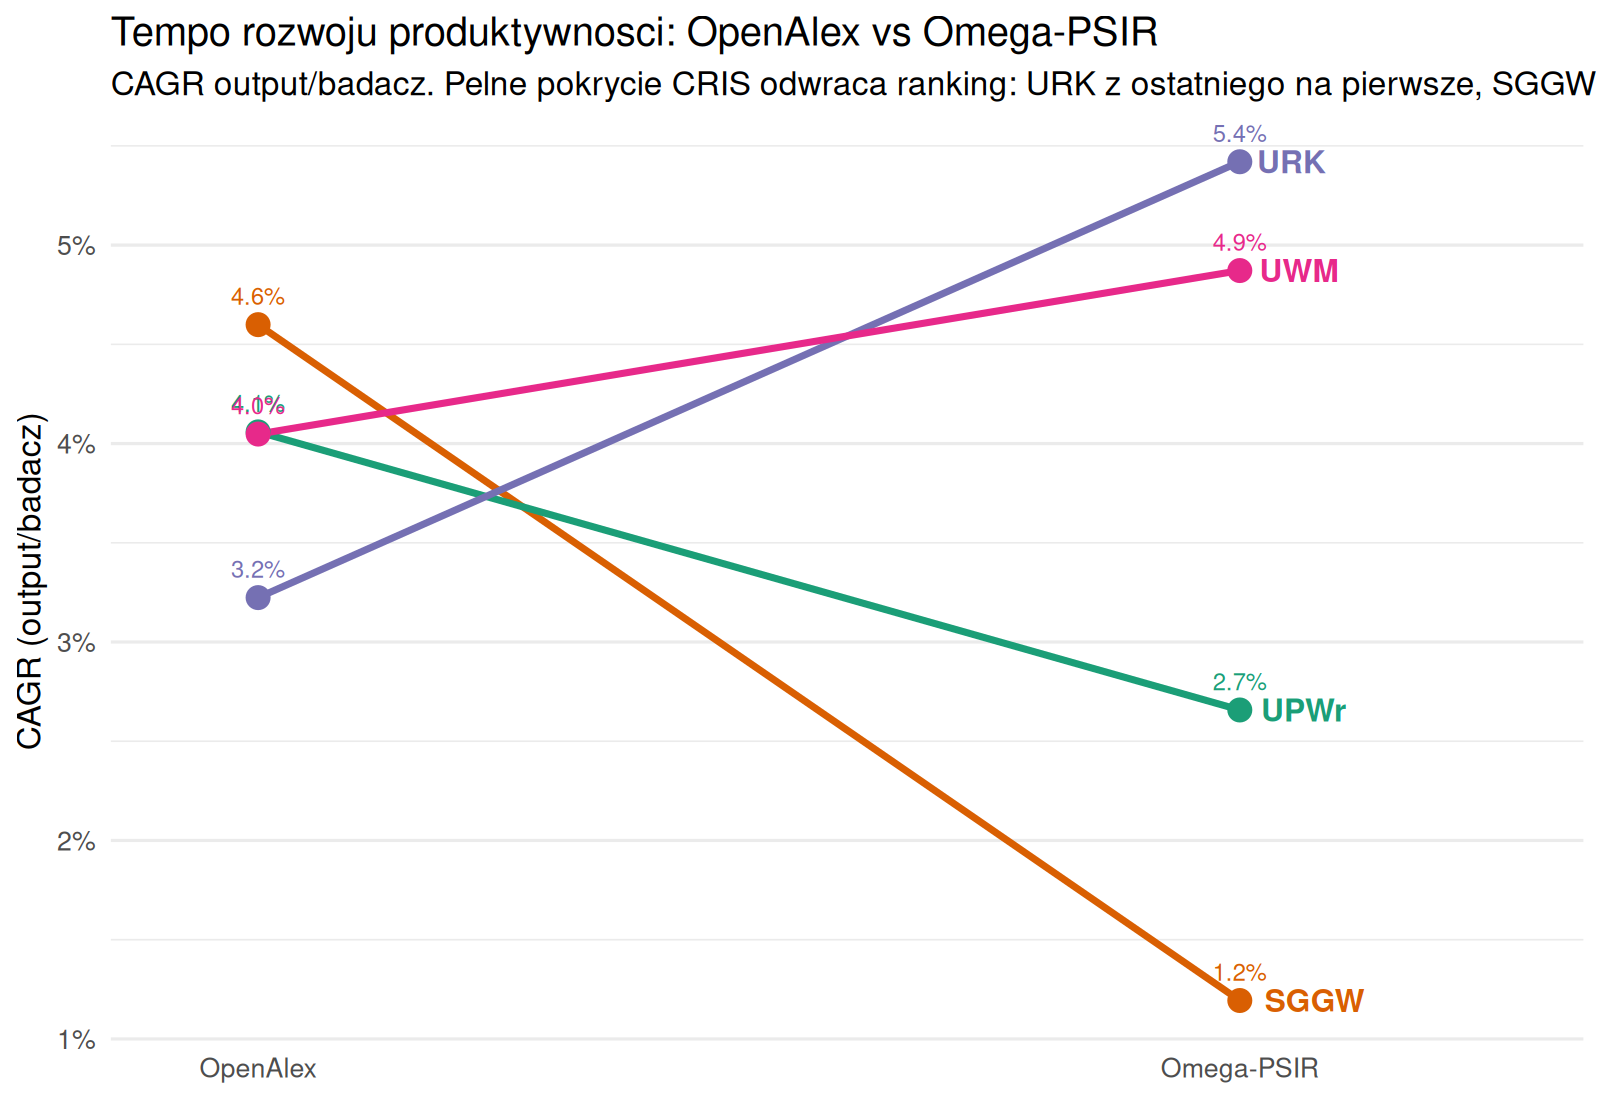
\includegraphics[width=0.8\linewidth,height=\textheight,keepaspectratio]{../Wykresy/praca/fig_06_dynamika_porownanie.png}

}

\caption{\label{fig-dynamika}Roczne tempo wzrostu liczby publikacji na
badacza według danych OpenAlex i Omega-PSIR. Linie pokazują 95\%
przedziały ufności. Wyniki wskazują, że ocena dynamiki rozwoju uczelni
zależy od źródła danych.}

\end{figure}%

Różnice między wynikami z OpenAlex i Omega-PSIR nie wynikają przede
wszystkim z problemów z dopasowaniem autorów do OpenAlex. Po poprawieniu
dopasowania URK z 47,5 \% do 77,8 \% wyniki OpenAlex nadal pokazują
bardzo podobne tempo wzrostu we wszystkich uczelniach, na poziomie około
4 \%. Natomiast pełne dane z Omega-PSIR ujawniają większe różnice między
uczelniami, od 1,2 \% do 5,4 \%. Oznacza to, że głównym źródłem
rozbieżności jest raczej niepełne pokrycie publikacji w OpenAlex niż sam
błąd dopasowania autorów.

OpenAlex nie obejmuje wszystkich publikacji widocznych w systemach
Omega-PSIR, zwłaszcza części publikacji w polskich czasopismach i
monografii. Dlatego może zaniżać lub zniekształcać obraz dorobku,
szczególnie w analizach porównujących uczelnie.

Wynik ten potwierdza główne założenie metodyczne pracy: w porównaniach
międzyuczelnianych ważna jest nie tylko dostępność danych, ale także ich
kompletność i porównywalność. Ten sam wskaźnik tempa rozwoju prowadzi do
innych wniosków w zależności od źródła danych.

Różnice między uczelniami należy jednak interpretować ostrożnie,
ponieważ przedziały ufności są szerokie i częściowo się nakładają.
Bardziej wiarygodny jest ogólny podział na uczelnie o wyższym tempie
wzrostu (URK, UWM) oraz uczelnie o bardziej ustabilizowanej
produktywności (UPWr, SGGW), niż dokładny ranking uczelni.

\subsection{Ograniczenia badania}\label{ograniczenia-badania}

\begin{itemize}
\tightlist
\item
  Wskaźniki bibliometryczne nie odtwarzają oficjalnej ewaluacji. Analiza
  opiera się na zagregowanych wskaźnikach przypisanych do autorów,
  takich jak liczba publikacji, h-index, sumaryczny IF czy punktacja
  MEiN. Wskaźniki te przybliżają indywidualny dorobek naukowy, ale nie
  odtwarzają oficjalnego algorytmu ewaluacji jakości działalności
  naukowej. Oficjalna ewaluacja działa na poziomie uczelni i dyscypliny,
  uwzględnia udziały jednostkowe autorów, sloty publikacyjne oraz
  punktację ministerialną, a nie Impact Factor
  (\citeproc{ref-rozp_ewaluacja2022}{Minister Edukacji i Nauki 2022}).
  Wyników nie należy więc bezpośrednio przekładać na kategorie
  ewaluacyjne uczelni.
\item
  Kategoria ewaluacyjna jest powiązana z uczelnią. W badanej próbie
  tylko UWM ma kategorię B+, a pozostałe trzy uczelnie mają kategorię A.
  Nie można więc oddzielić wpływu kategorii ewaluacyjnej od specyfiki
  konkretnej uczelni. Z tego powodu kategorię MEiN potraktowano
  wyłącznie opisowo.
\item
  Nie wszystkie uczelnie udostępniają te same metryki. SGGW nie
  udostępnia sumarycznej punktacji MEiN, a UWM nie udostępnia wskaźnika
  SNIP. Dlatego część analiz musiała zostać ograniczona do uczelni, dla
  których dane były dostępne. Ogranicza to porównywalność niektórych
  wskaźników między uczelniami.
\item
  Punktacja MEiN zmieniała się w czasie. Sumaryczna punktacja MEiN
  obejmuje publikacje oceniane według różnych zasad i wykazów czasopism.
  Dane z systemu Omega-PSIR podają ją jako jedną wartość zbiorczą, bez
  rozbicia na okresy. Nie można więc sprawdzić, jak zmiany zasad
  punktacji wpływały na wynik poszczególnych osób.
\item
  Dopasowanie do OpenAlex nie było pełne. Średnio do OpenAlex dopasowano
  79,4 \% badaczy. Najniższy poziom dopasowania wystąpił w UWM (67,1
  \%). Oznacza to, że metryki pochodzące z OpenAlex, takie jak FWCI i
  dane o współautorstwie, dotyczą tylko części próby i mogą być
  obciążone brakami danych. Dopasowanie miało przy tym charakter
  automatyczny (filtr ROR + próg Jaro-Winklera), bez ręcznej weryfikacji
  każdego rekordu, co przy nazwiskach popularnych może być źródłem
  pojedynczych błędnych przypisań.
\item
  Dane mają charakter przekrojowy. Analiza pokazuje stan dorobku osób
  zatrudnionych w momencie pozyskania danych. Wskaźniki takie jak
  h-index, liczba publikacji i sumaryczny IF rosną wraz ze stażem,
  dlatego część różnic między stanowiskami może wynikać po prostu z
  długości kariery naukowej.
\item
  Model ilościowy miał małą klasę pozytywną. W modelu przewidującym
  wysoki wpływ publikacyjny grupa pozytywna liczyła 46 osób. Mimo
  zastosowania walidacji krzyżowej i kalibracji progu wyniki tego modelu
  należy traktować jako orientacyjne.
\item
  Próg klasy w modelu ilościowym wyznaczono na pełnej próbie. Granicę
  górnego decyla sumarycznego IF policzono na całym zbiorze przed
  podziałem na część uczącą i testową, co może nieznacznie
  optymistycznie obciążać ocenę tego modelu. Model jakościowy jest wolny
  od tego problemu, ponieważ próg FWCI = 1 jest stałą zewnętrzną
  (średnia światowa w dziedzinie), niezależną od rozkładu wartości w
  próbie.
\item
  Model jakościowy opierał się tylko na osobach dopasowanych do
  OpenAlex. Model FWCI \textgreater{} 1 obejmował 366 osób, czyli tylko
  część próby. Także wiek akademicki, liczony na podstawie pierwszej
  publikacji w OpenAlex, jest przybliżeniem rzeczywistego stażu badacza.
\item
  Analiza dynamiki ma charakter eksploracyjny. Tempo rozwoju liczono dla
  osób obecnych w badanej próbie. Nie uwzględnia ono osób, które
  wcześniej pracowały w uczelni, ale odeszły lub przeszły na emeryturę
  przed scrapingiem. Analiza opisuje więc historię dorobku obecnej
  kadry, a nie pełną historię instytucji. Z tego powodu wyniki dynamiki
  należy traktować jako sygnał kierunkowy, a nie ścisły ranking uczelni.
\item
  OpenAlex nie obejmuje pełnego polskiego dorobku. Część polskich
  czasopism, monografii i innych publikacji widocznych w Omega-PSIR może
  nie być indeksowana w OpenAlex; pokrycie OpenAlex względem baz
  komercyjnych było przedmiotem osobnych analiz porównawczych
  (\citeproc{ref-culbertReferenceCoverageAnalysis2025}{Culbert i in.
  2025}). Dlatego Omega-PSIR przyjęto jako źródło podstawowe, a OpenAlex
  jako źródło uzupełniające.
\end{itemize}

\section{Wnioski}\label{wnioski}

\begin{enumerate}
\def\labelenumi{\arabic{enumi}.}
\tightlist
\item
  Typologia profili bibliometrycznych (pytanie 1). Wśród badanych
  naukowców można wyróżnić dwa główne typy profili bibliometrycznych:
  grupę badaczy o wysokim dorobku publikacyjnym, obejmującą około 23 \%
  próby, oraz pozostałych badaczy. Podział ten powtarza się w podobnej
  formie w poszczególnych uczelniach, choć nie wszędzie z taką samą
  stabilnością. W UPWr grupa o wysokim dorobku ma bardziej ilościowy
  charakter, ponieważ wyróżnia ją przede wszystkim liczba publikacji. W
  UWM lokalny podział jest mniej stabilny, co wynika prawdopodobnie z
  mniejszej liczebności próby.
\item
  Różnice między stanowiskami i uczelniami (pytanie 2). Wskaźniki
  bibliometryczne są silniej związane ze stanowiskiem niż z uczelnią. W
  większości przypadków rosną one wraz z poziomem stanowiska: od
  adiunktów, przez profesorów uczelni, do profesorów. Uczelnia ma
  słabsze znaczenie. Oznacza to, że etap kariery naukowej lepiej
  wyjaśnia różnice w indywidualnym dorobku niż sama afiliacja
  uczelniana.
\item
  Przewidywanie wysokiego wpływu publikacyjnego (pytanie 3). Wysoki
  wpływ publikacyjny można dobrze przewidywać na podstawie cech badacza.
  Model osiągnął wysoką zdolność rozróżniania osób o wysokim i niższym
  wpływie publikacyjnym (AUC ok. 0,97). Najważniejsze były liczba
  publikacji oraz cechy współpracy naukowej, a nie formalne stanowisko
  czy uczelnia. Wyniki predykcyjne należy jednak traktować ostrożnie,
  ponieważ grupa osób o wysokim wpływie była mała (46 przypadków), a
  model wymagał kalibracji progu klasyfikacji.
\item
  Sieć współautorstwa (pytanie 4). Sieć współautorstwa dzieli się na
  wyraźne grupy współpracy (Q = 0,856). Grupy te pokrywają się głównie z
  uczelnią (NMI = 0,58), a nie ze stanowiskiem. Oznacza to, że
  współpraca naukowa w badanej dyscyplinie ma przede wszystkim charakter
  wewnątrzuczelniany, a współprace międzyuczelniane są rzadsze.
\end{enumerate}

Łącznie wyniki pokazują, że indywidualny dorobek naukowców jest związany
głównie z etapem kariery, natomiast współpraca naukowa przebiega przede
wszystkim w obrębie uczelni. Praca potwierdza także znaczenie
jednorodnego źródła danych. Wykorzystanie systemów Omega-PSIR umożliwiło
porównywalne pozyskanie wskaźników bibliometrycznych z czterech uczelni,
co byłoby znacznie trudniejsze przy użyciu różnych, niejednolitych
repozytoriów.

\subsection{Wnioski dla praktyki}\label{wnioski-dla-praktyki}

Wyniki badania mogą być użyteczne dla osób i instytucji odpowiedzialnych
za systemy informacji o nauce, a także dla rad dyscypliny rolnictwo i
ogrodnictwo. Mogą one wspierać lepsze rozpoznanie struktury dorobku,
zakresu współpracy oraz tempa rozwoju naukowego w obrębie tej
dyscypliny. Należy je jednak traktować jako sugestie, a nie gotowe
rekomendacje, ponieważ analiza ma charakter obserwacyjny i przekrojowy,
a dane OpenAlex nie obejmują pełnego dorobku badanych osób.

Po pierwsze, wyniki pokazują, że kompletność i jednorodność systemu CRIS
są ważne dla wiarygodnych porównań między uczelniami. Analiza dynamiki
publikacyjnej wykazała, że ten sam wskaźnik może prowadzić do innych
wniosków w zależności od źródła danych. OpenAlex i pełne dane Omega-PSIR
dały odmienne wyniki, co pokazuje, że opieranie porównań wyłącznie na
globalnych bazach może być ryzykowne, zwłaszcza gdy nie obejmują one
części polskich czasopism i monografii.

Po drugie, porównywalność danych utrudnia to, że poszczególne uczelnie
nie udostępniają tych samych metryk w taki sam sposób. Brak zagregowanej
punktacji MEiN w SGGW oraz brak wskaźnika SNIP w UWM ograniczyły część
analiz. Dlatego przydatne byłoby udostępnianie podstawowych metryk,
takich jak sumaryczny IF, SNIP, punktacja MEiN i h-index, w jednolitej
oraz maszynowo dostępnej formie. Wskazuje to na potrzebę odgórnej
standaryzacji struktur danych i interfejsów udostępniania wskaźników we
wdrożeniach systemów klasy CRIS na polskich uczelniach, tak aby krajowa
agregacja kluczowych metryk (w tym punktacji MEiN) nie wymagała
tworzenia osobnych reguł mapowania dla poszczególnych jednostek.

Po trzecie, wyniki sugerują, że wysoka jakość dorobku nie musi być
związana wyłącznie z długim stażem czy dużą liczbą publikacji. W
analizie widoczna była grupa młodszych badaczy o wysokich wskaźnikach
jakościowych. Ich wyniki wiązały się przede wszystkim z udziałem w
szerszej, wieloautorskiej współpracy. Wniosek ten wymaga jednak
potwierdzenia w badaniach podłużnych, zanim mógłby zostać wykorzystany
jako podstawa praktycznych zaleceń dotyczących budowania zespołów
badawczych.

\newpage{}

\section{Bibliografia}\label{bibliografia}

\phantomsection\label{refs}
\begin{CSLReferences}{1}{0}
\bibitem[\citeproctext]{ref-ariaBibliometrix2017}
Aria, Massimo, i Corrado Cuccurullo. 2017. {„bibliometrix: An {R}-tool
for comprehensive science mapping analysis''}. \emph{Journal of
Informetrics} 11 (4): 959--75.
\url{https://doi.org/10.1016/j.joi.2017.08.007}.

\bibitem[\citeproctext]{ref-ariaOpenalexR2024}
Aria, Massimo, Trang Le, Corrado Cuccurullo, Alessandra Belfiore, i June
Choe. 2024. {„{openalexR}: An {R}-Tool for Collecting Bibliometric Data
from {OpenAlex}''}. \emph{The R Journal} 15 (4): 167--80.
\url{https://doi.org/10.32614/RJ-2023-089}.

\bibitem[\citeproctext]{ref-blondel2008}
Blondel, Vincent D., Jean-Loup Guillaume, Renaud Lambiotte, i Etienne
Lefebvre. 2008. {„Fast unfolding of communities in large networks''}.
\emph{Journal of Statistical Mechanics: Theory and Experiment} 2008
(10): P10008.

\bibitem[\citeproctext]{ref-breiman2001}
Breiman, Leo. 2001. {„Random forests''}. \emph{Machine Learning} 45 (1):
5--32.

\bibitem[\citeproctext]{ref-chen2016}
Chen, Tianqi, i Carlos Guestrin. 2016. {„{XGBoost}: A scalable tree
boosting system''}. W \emph{Proceedings of the 22nd ACM SIGKDD
International Conference on Knowledge Discovery and Data Mining},
785--94.

\bibitem[\citeproctext]{ref-culbertReferenceCoverageAnalysis2025}
Culbert, Jack H., Anne Hobert, Najko Jahn, Nick Haupka, Marion Schmidt,
Paul Donner, i Philipp Mayr. 2025. {„Reference coverage analysis of
{OpenAlex} compared to {Web of Science} and {Scopus}''}.
\emph{Scientometrics} 130 (4): 2475--92.
\url{https://doi.org/10.1007/s11192-025-05293-3}.

\bibitem[\citeproctext]{ref-Drabek2012}
Drabek, Aneta. 2012. {„Wykorzystanie bibliometrii w polityce
naukowej''}. \emph{Biuletyn EBIB} 130 (3).

\bibitem[\citeproctext]{ref-garfield2006}
Garfield, Eugene. 2006. {„The history and meaning of the journal impact
factor''}. \emph{JAMA} 295 (1): 90--93.

\bibitem[\citeproctext]{ref-Grygiel2009}
Grygiel, Paweł, Sławomir Rębisz, i Grzegorz Humenny. 2009. {„Analiza
bibliometryczna jako narzędzie badania efektywności nauczycieli
akademickich na przykładzie {Uniwersytetu Rzeszowskiego}''}.
\emph{Zarządzanie Publiczne} 7 (3): 65--84.

\bibitem[\citeproctext]{ref-hicksBibliometricsLeidenManifesto2015}
Hicks, Diana, Paul Wouters, Ludo Waltman, Sarah de Rijcke, i Ismael
Rafols. 2015. {„Bibliometrics: The {Leiden Manifesto} for research
metrics''}. \emph{Nature} 520 (7548): 429--31.
\url{https://doi.org/10.1038/520429a}.

\bibitem[\citeproctext]{ref-hirsch2005}
Hirsch, Jorge E. 2005. {„An index to quantify an individual's scientific
research output''}. \emph{Proceedings of the National Academy of
Sciences} 102 (46): 16569--72.

\bibitem[\citeproctext]{ref-hubert1985}
Hubert, Lawrence, i Phipps Arabie. 1985. {„Comparing partitions''}.
\emph{Journal of Classification} 2 (1): 193--218.

\bibitem[\citeproctext]{ref-koperwas2015omega}
Koperwas, Jakub, Łukasz Skonieczny, Henryk Rybiński, i Wacław Struk.
2015. {„{OMEGA-PSIR} -- a solution for implementing university research
knowledge base''}. W \emph{Proceedings of the 21st EUNIS Congress}.
Dundee: European University Information Systems Organisation (EUNIS).
\url{https://dspacecris.eurocris.org/handle/11366/446}.

\bibitem[\citeproctext]{ref-Kulczycki2019}
Kulczycki, Emanuel. 2019. {„Tajemnice bibliometrii''}. \emph{Forum
Akademickie}, nr 6.

\bibitem[\citeproctext]{ref-lundberg2017}
Lundberg, Scott M., i Su-In Lee. 2017. {„A unified approach to
interpreting model predictions''}. W \emph{Advances in Neural
Information Processing Systems}, 30:4765--74.

\bibitem[\citeproctext]{ref-rozp_ewaluacja2022}
Minister Edukacji i Nauki. 2022. {„Obwieszczenie Ministra Edukacji i
Nauki z dnia 23 lutego 2022 r. w sprawie ogłoszenia jednolitego tekstu
rozporządzenia Ministra Nauki i Szkolnictwa Wyższego w sprawie ewaluacji
jakości działalności naukowej''}. Dz.U. 2022 poz. 661.

\bibitem[\citeproctext]{ref-rozp_dyscypliny2025}
Minister Nauki i Szkolnictwa Wyższego. 2025a. {„Obwieszczenie Ministra
Nauki i Szkolnictwa Wyższego z dnia 12 lutego 2025 r. w sprawie
ogłoszenia jednolitego tekstu rozporządzenia Ministra Edukacji i Nauki w
sprawie dziedzin nauki i dyscyplin naukowych oraz dyscyplin
artystycznych''}. Dz.U. 2025 poz. 211.

\bibitem[\citeproctext]{ref-rozp_ewaluacja_nowela2025}
---------. 2025b. {„Rozporządzenie Ministra Nauki i Szkolnictwa Wyższego
z dnia 30 lipca 2025 r. zmieniające rozporządzenie w sprawie ewaluacji
jakości działalności naukowej''}. Dz.U. 2025 poz. 1053.

\bibitem[\citeproctext]{ref-moed2010snip}
Moed, Henk F. 2010. {„Measuring contextual citation impact of scientific
journals''}. \emph{Journal of Informetrics} 4 (3): 265--77.

\bibitem[\citeproctext]{ref-newmanCoauthorshipNetworksPatterns2004}
Newman, Mark E. J. 2004. {„Coauthorship networks and patterns of
scientific collaboration''}. \emph{Proceedings of the National Academy
of Sciences} 101 (suppl 1): 5200--5205.
\url{https://doi.org/10.1073/pnas.0307545100}.

\bibitem[\citeproctext]{ref-newman2006}
---------. 2006. {„Modularity and community structure in networks''}.
\emph{Proceedings of the National Academy of Sciences} 103 (23):
8577--82.

\bibitem[\citeproctext]{ref-Opalinski2017}
Opaliński, Łukasz. 2017. {„Bibliometryczna metodologia prognozowania i
oceny rozwoju dyscyplin naukowych. Analiza piśmiennictwa. Część 1''}.
\emph{Zagadnienia Informacji Naukowej} 55 (1): 34--65.

\bibitem[\citeproctext]{ref-openalex2022}
Priem, Jason, Heather Piwowar, i Richard Orr. 2022. {„OpenAlex: A
fully-open index of scholarly works, authors, venues, institutions, and
concepts''}. \emph{arXiv preprint arXiv:2205.01833}.

\bibitem[\citeproctext]{ref-rybinskiOmegaPSIRInstitutionalCRIS2018}
Rybiński, Henryk, Weronika Kubrak, Łukasz Skonieczny, Jakub Koperwas, i
Wacław Struk. 2018. {„Omega-{PSIR}: {Institutional CRIS} at {Polish
Universities}''}. \emph{ITlib. Informačné technológie a knižnice}.
\url{https://doi.org/10.25610/itlib-2018-0005}.

\bibitem[\citeproctext]{ref-waltman2016review}
Waltman, Ludo. 2016. {„A review of the literature on citation impact
indicators''}. \emph{Journal of Informetrics} 10 (2): 365--91.

\bibitem[\citeproctext]{ref-omegapsir2024}
Warsaw University of Technology. 2024. {„Omega-PSIR: University Research
Information System''}. \url{https://www.omegapsir.io/}.

\bibitem[\citeproctext]{ref-winkler1990}
Winkler, William E. 1990. {„String comparator metrics and enhanced
decision rules in the {Fellegi-Sunter} model of record linkage''}.
\emph{Proceedings of the Section on Survey Research Methods, American
Statistical Association}, 354--59.

\bibitem[\citeproctext]{ref-youden1950}
Youden, W. J. 1950. {„Index for rating diagnostic tests''}.
\emph{Cancer} 3 (1): 32--35.

\end{CSLReferences}




\end{document}
